%------------------------------------------------------------------------------
\chapter{Thin Sensors}
\label{sec:appendix_ThinSensors}
%------------------------------------------------------------------------------

%% --------------------------------------------- %%
\section{Depletion voltage}

The measured depletion voltage for all the assemblies listed in
\cref{tab:Timepix3Assemblies}. \cref{sec:ThinSensors_depletionVoltage}
describes the method used for calculating the depletion.

\begin{figure}[htbp] \centering
  \begin{subfigure}[b]{0.33\textwidth}
    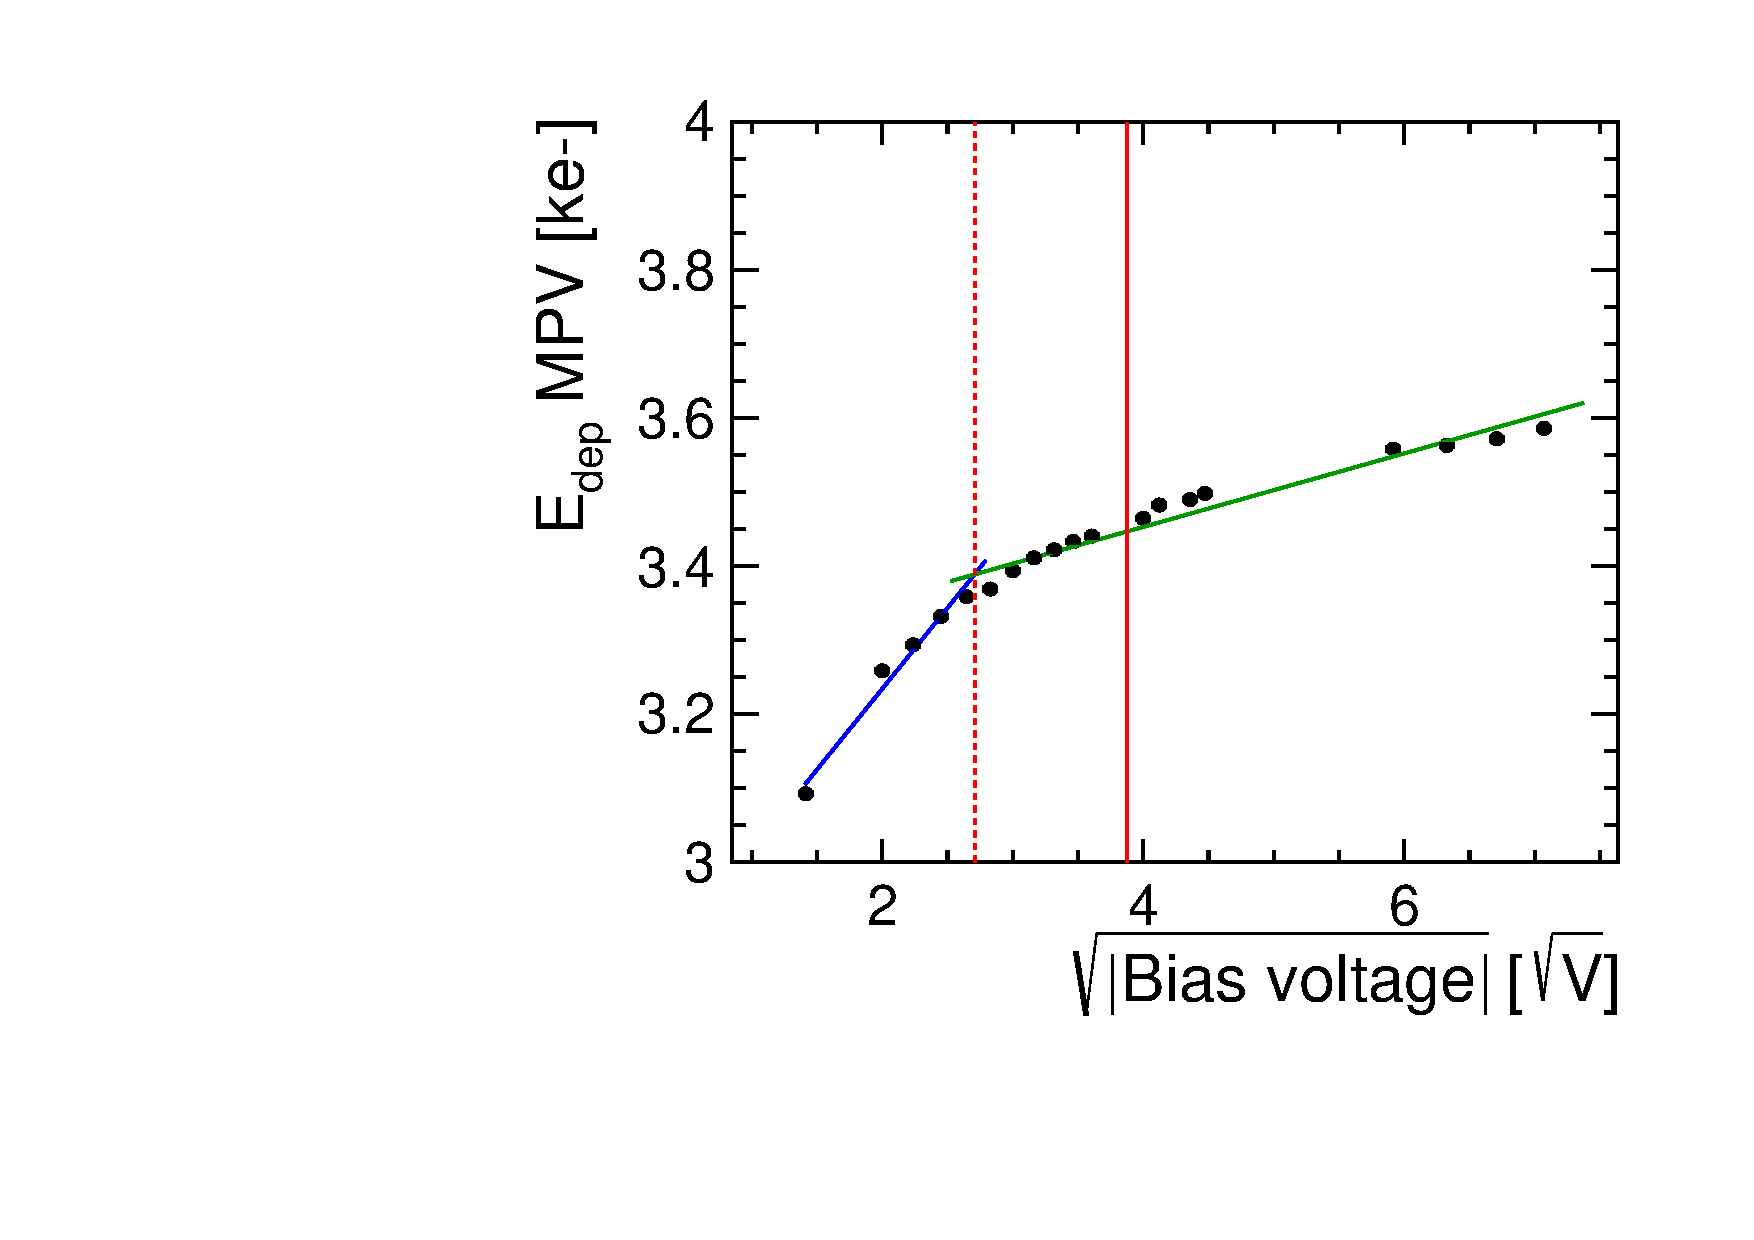
\includegraphics[width=\textwidth]{./figures/TestBeam/depletionVoltage_W0019_G07_Edep.pdf}
    \caption{W19\_G7}
  \end{subfigure} \hfill
  \begin{subfigure}[b]{0.33\textwidth}
    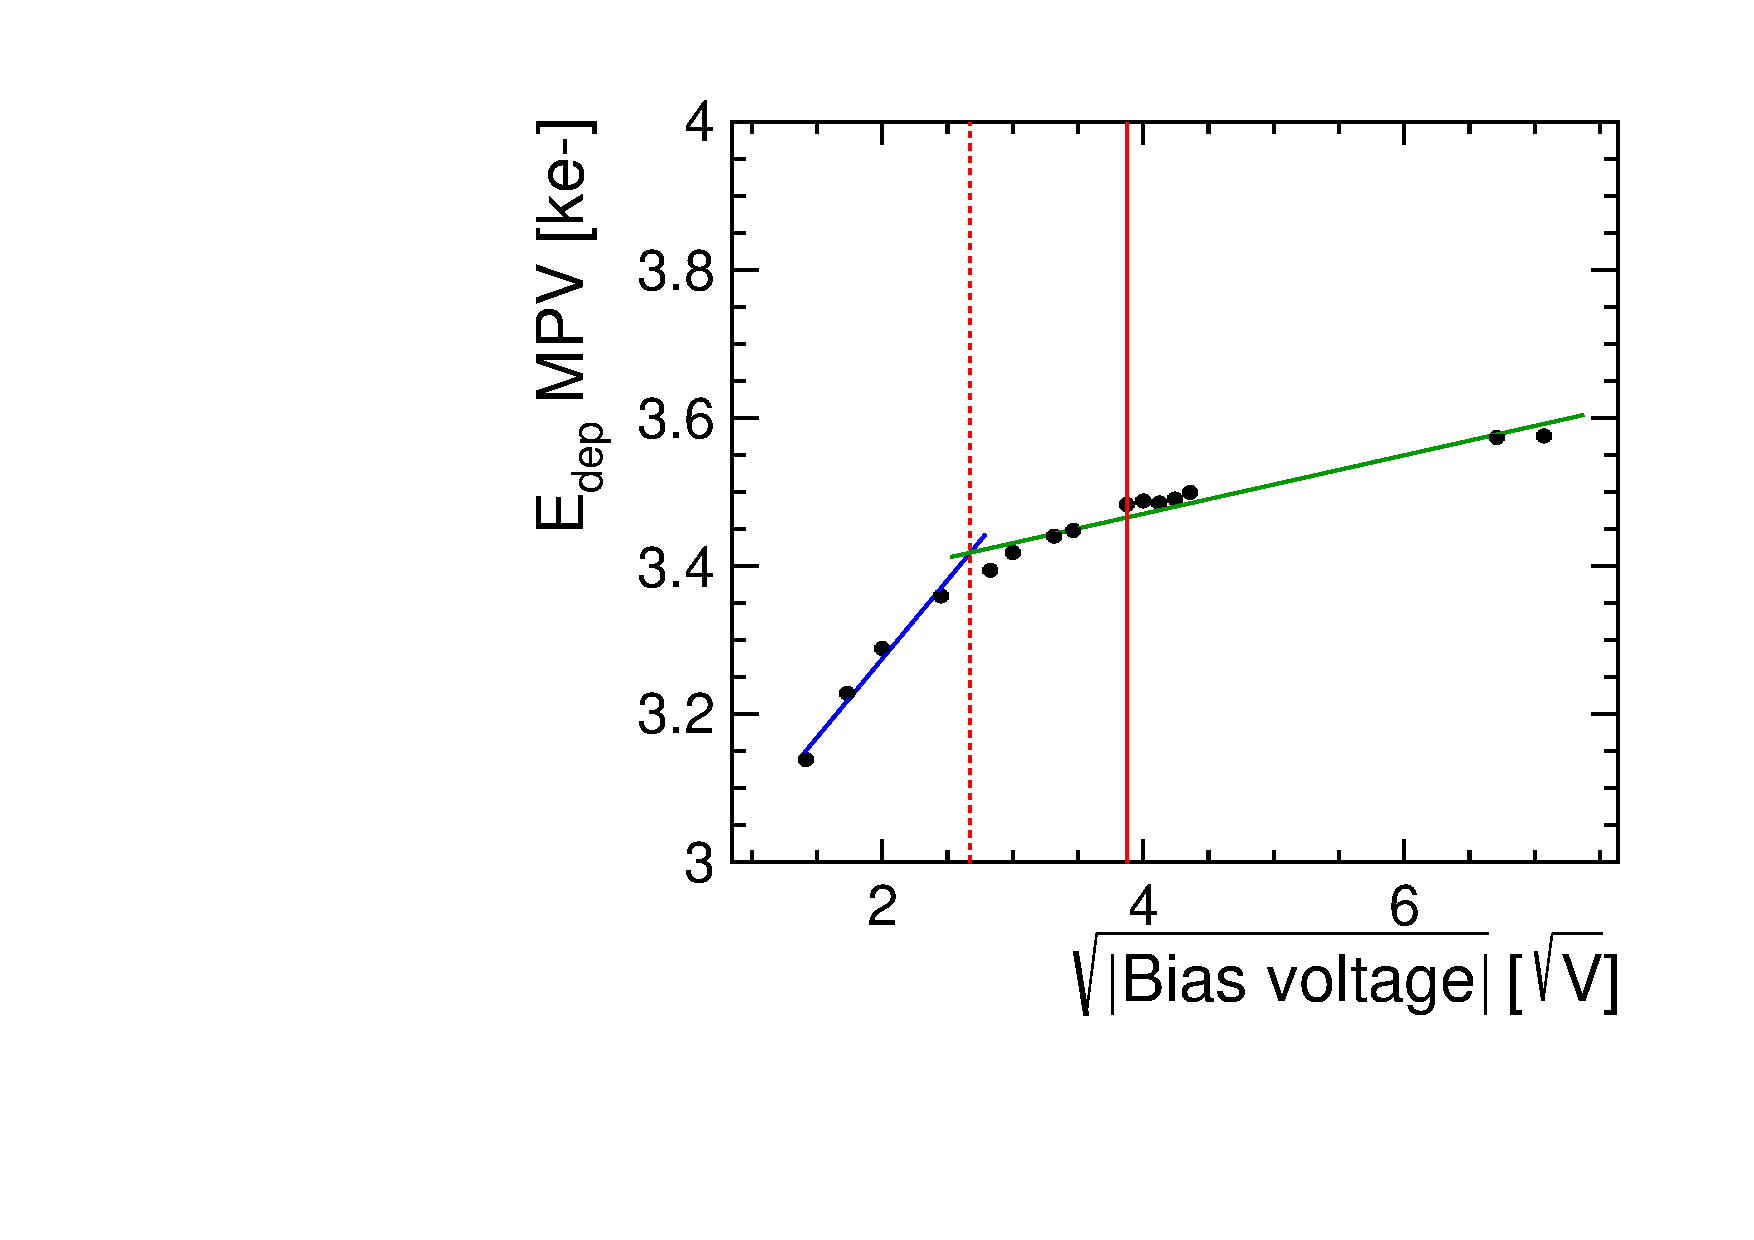
\includegraphics[width=\textwidth]{./figures/TestBeam/depletionVoltage_W0019_F07_Edep.pdf}
    \caption{W19\_F7}
  \end{subfigure}\hfill
  \begin{subfigure}[b]{0.33\textwidth}
    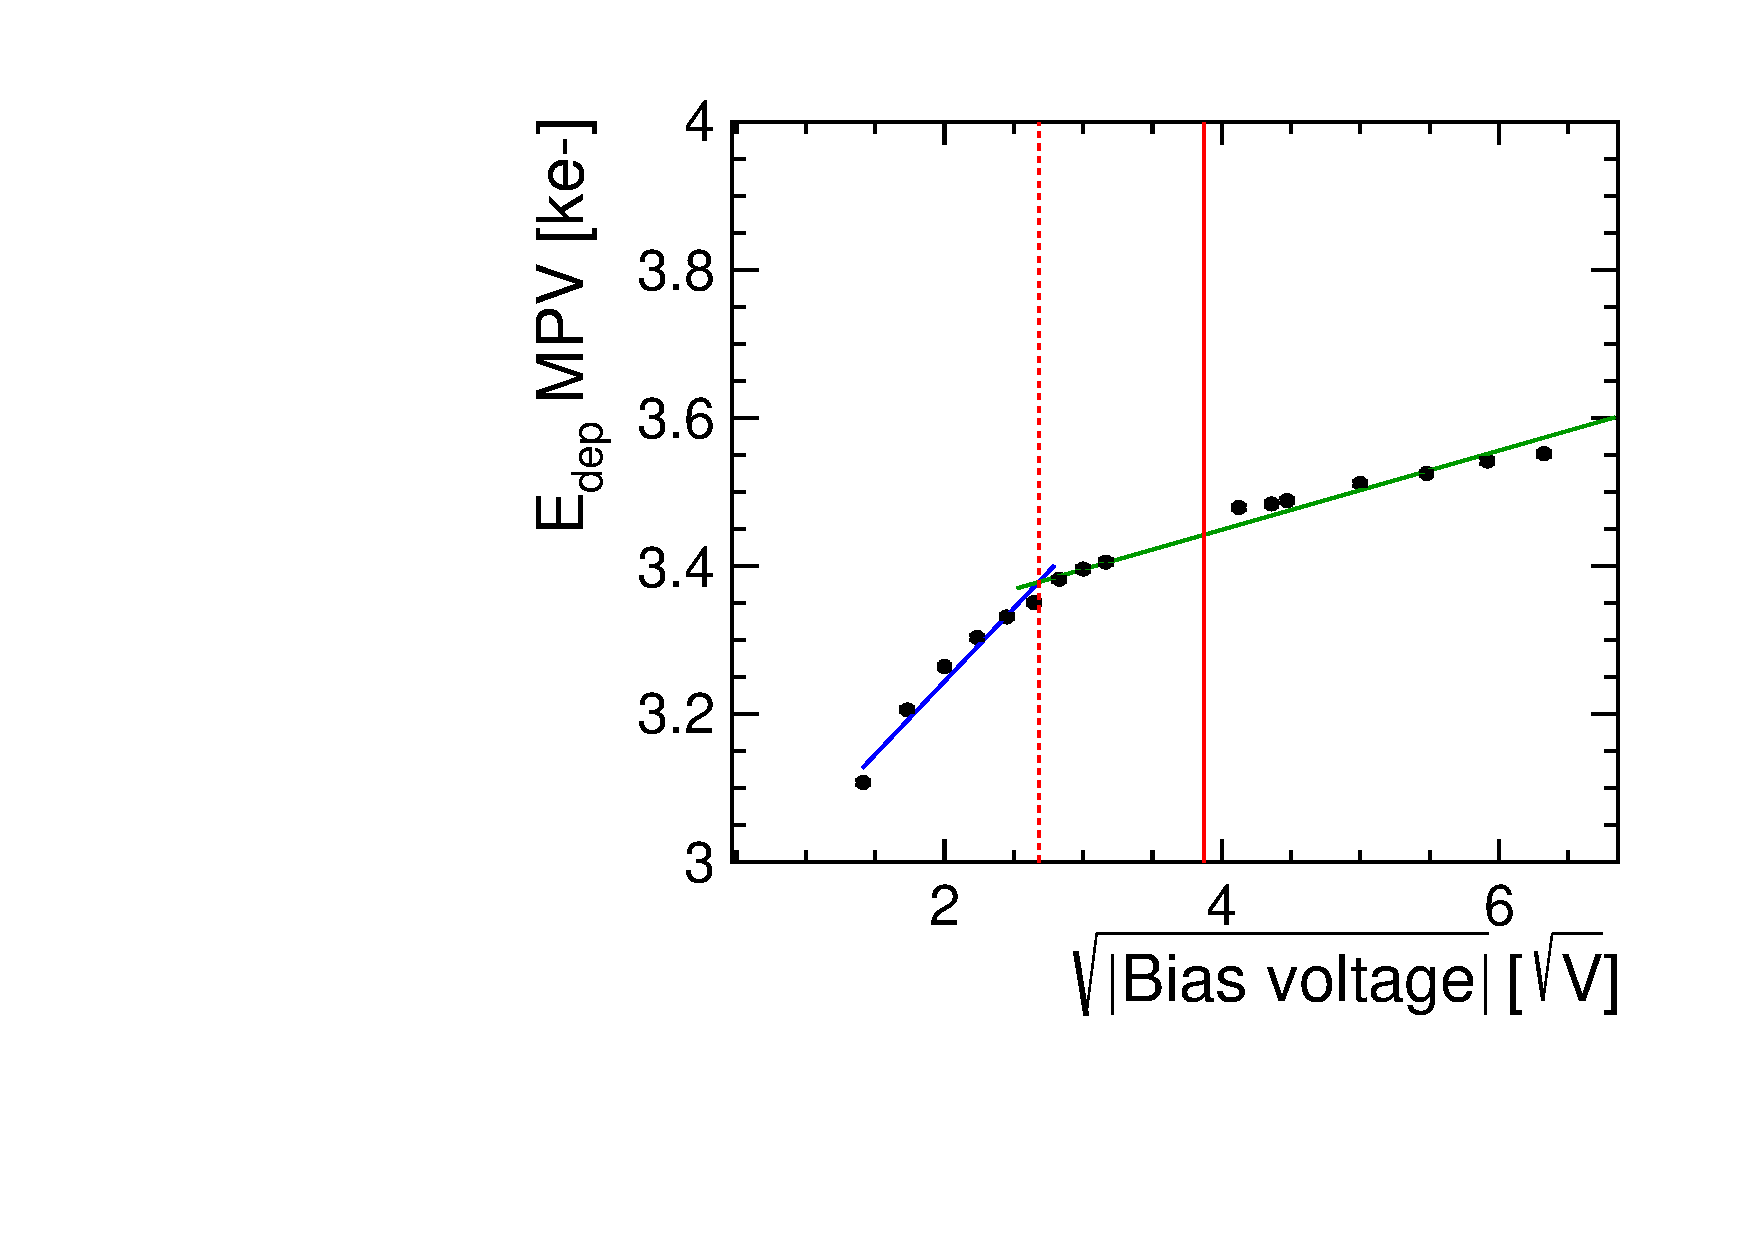
\includegraphics[width=\textwidth]{./figures/TestBeam/depletionVoltage_W0019_L08_Edep.pdf}
    \caption{W19\_L8}
  \end{subfigure} \\

  \begin{subfigure}[b]{0.33\textwidth}
    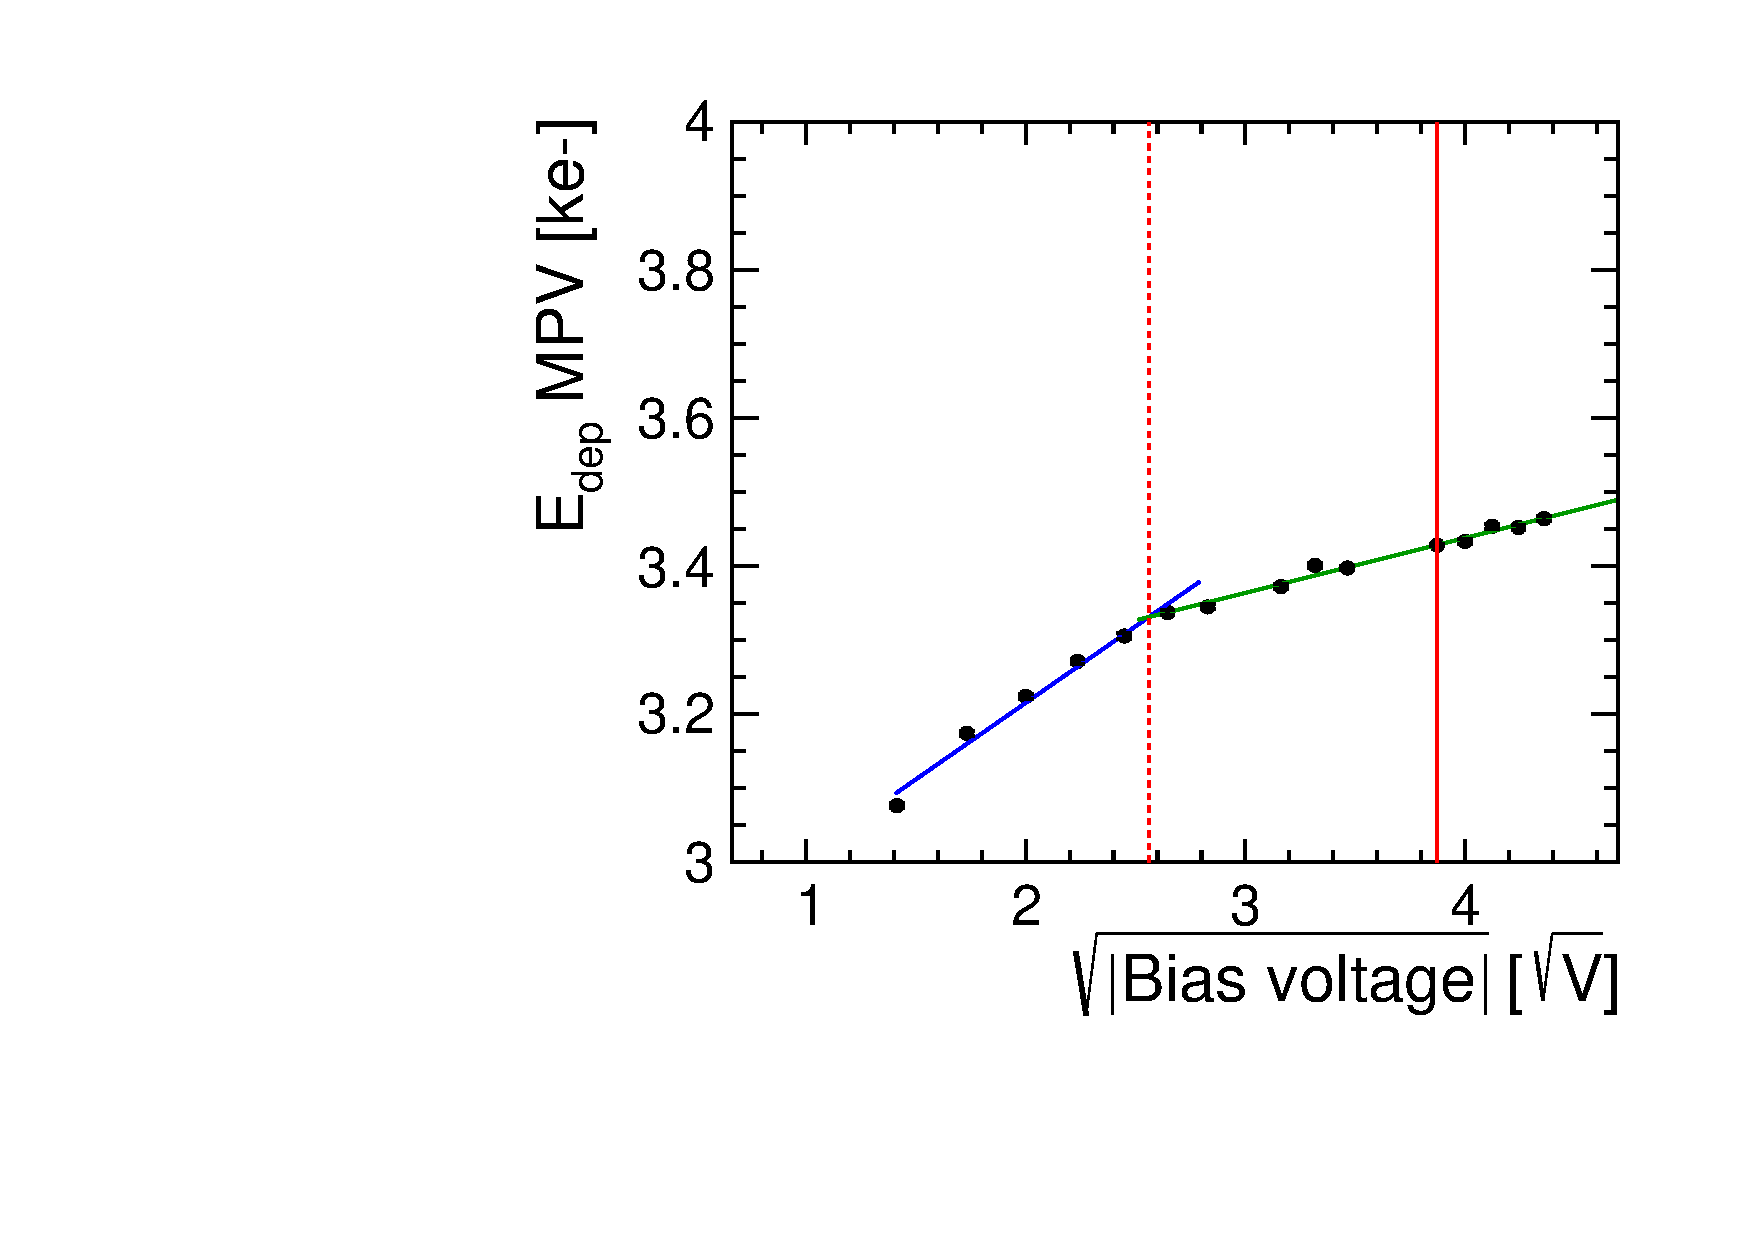
\includegraphics[width=\textwidth]{./figures/TestBeam/depletionVoltage_W0019_C07_Edep.pdf}
    \caption{W19\_C7}
  \end{subfigure} \hfill
  \begin{subfigure}[b]{0.33\textwidth}
    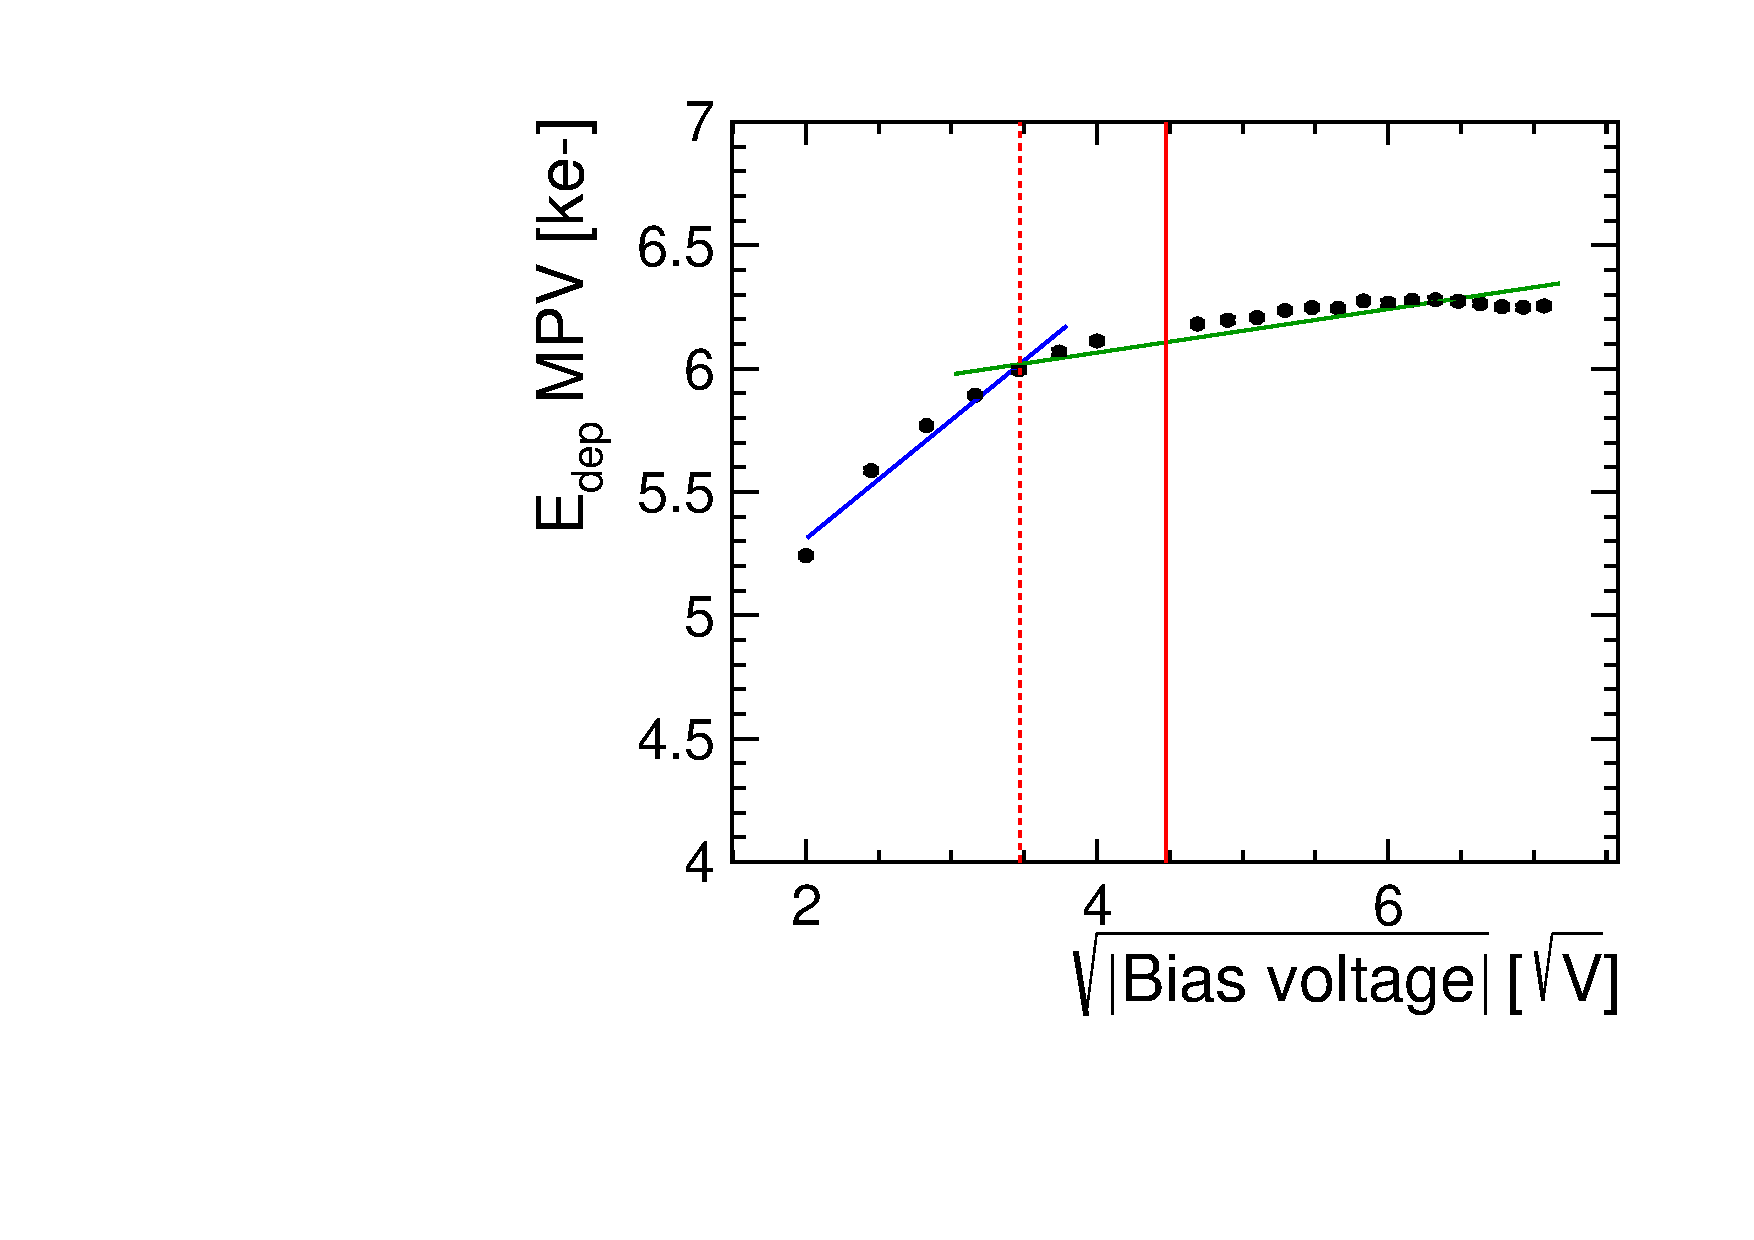
\includegraphics[width=\textwidth]{./figures/TestBeam/depletionVoltage_W0005_E02_Edep.pdf}
    \caption{W5\_E2}
  \end{subfigure}\hfill
  \begin{subfigure}[b]{0.33\textwidth}
    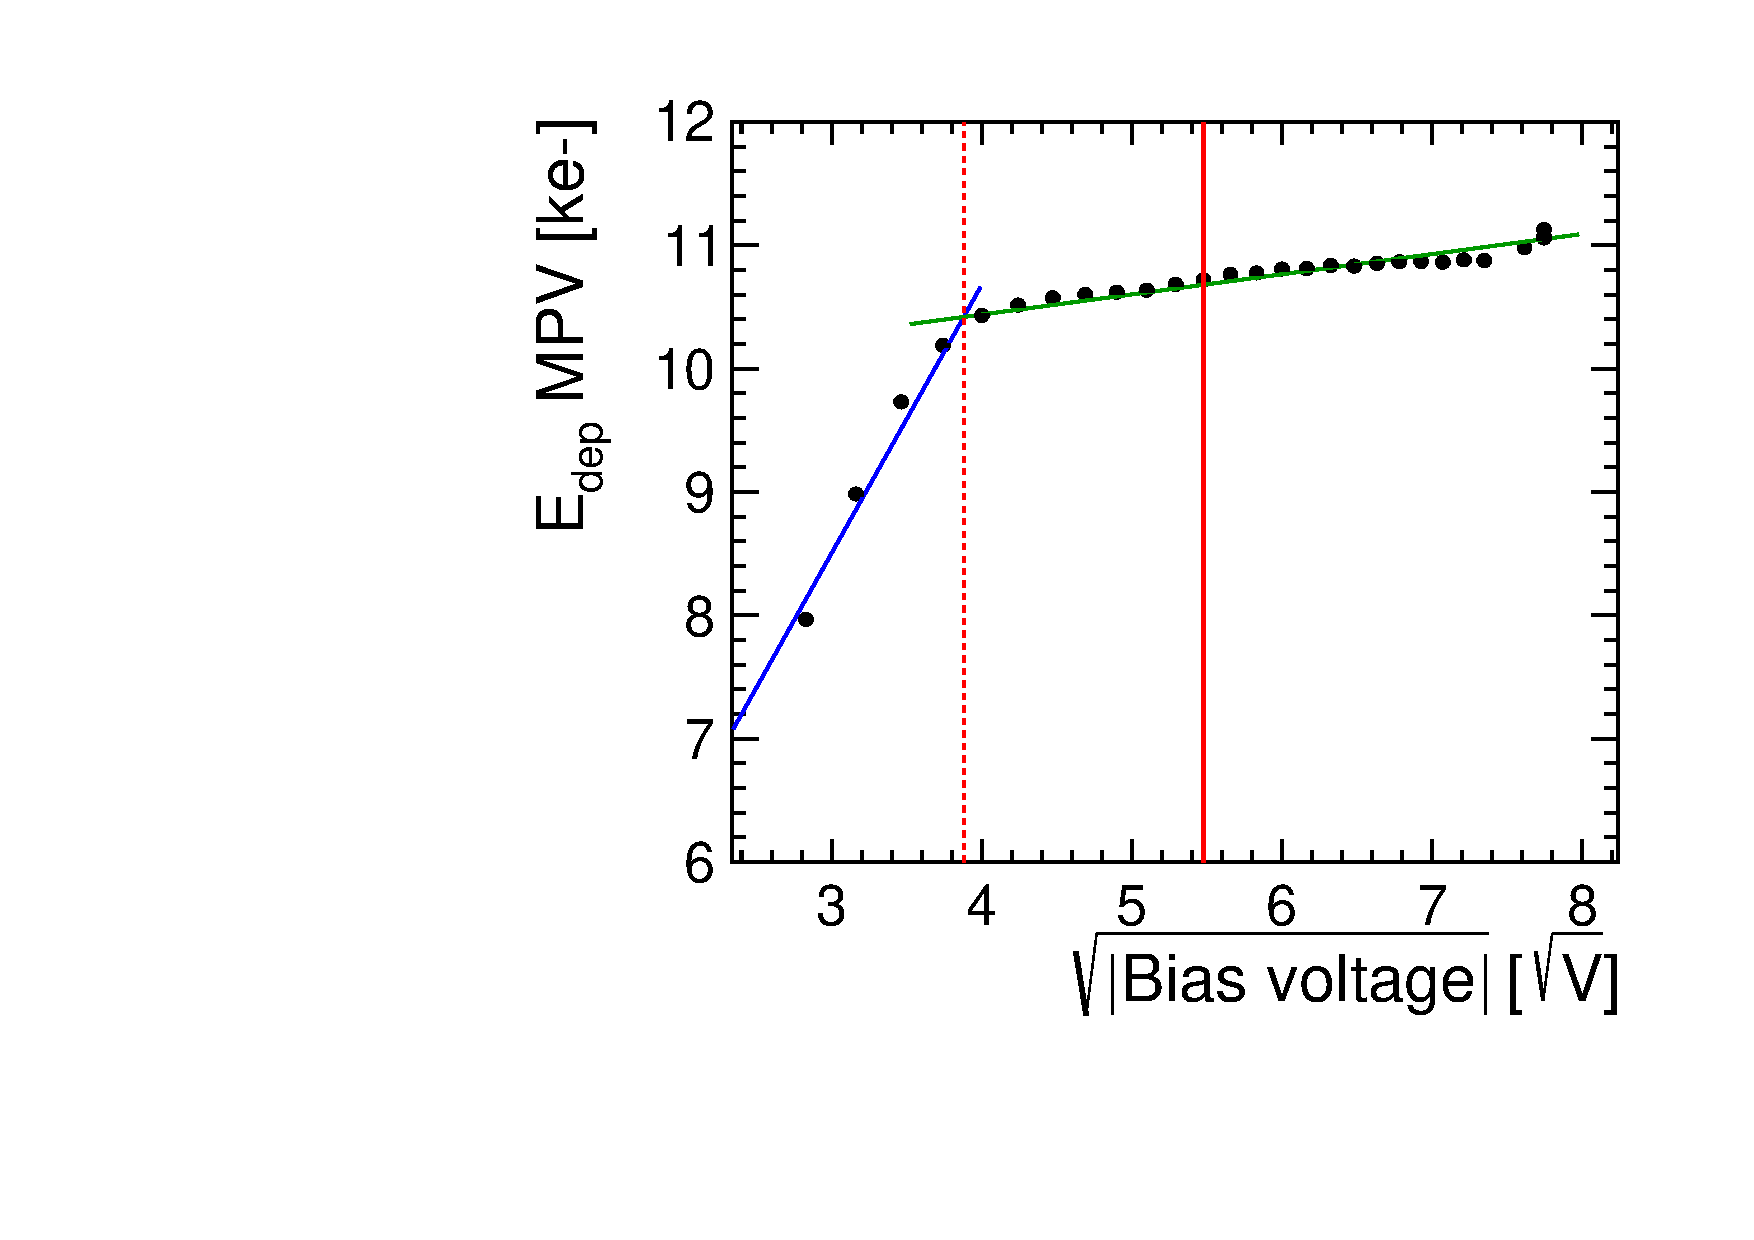
\includegraphics[width=\textwidth]{./figures/TestBeam/depletionVoltage_W0005_F01_Edep.pdf}
    \caption{W5\_F1}
  \end{subfigure}%\\
  % \begin{subfigure}[b]{0.33\textwidth}
  %   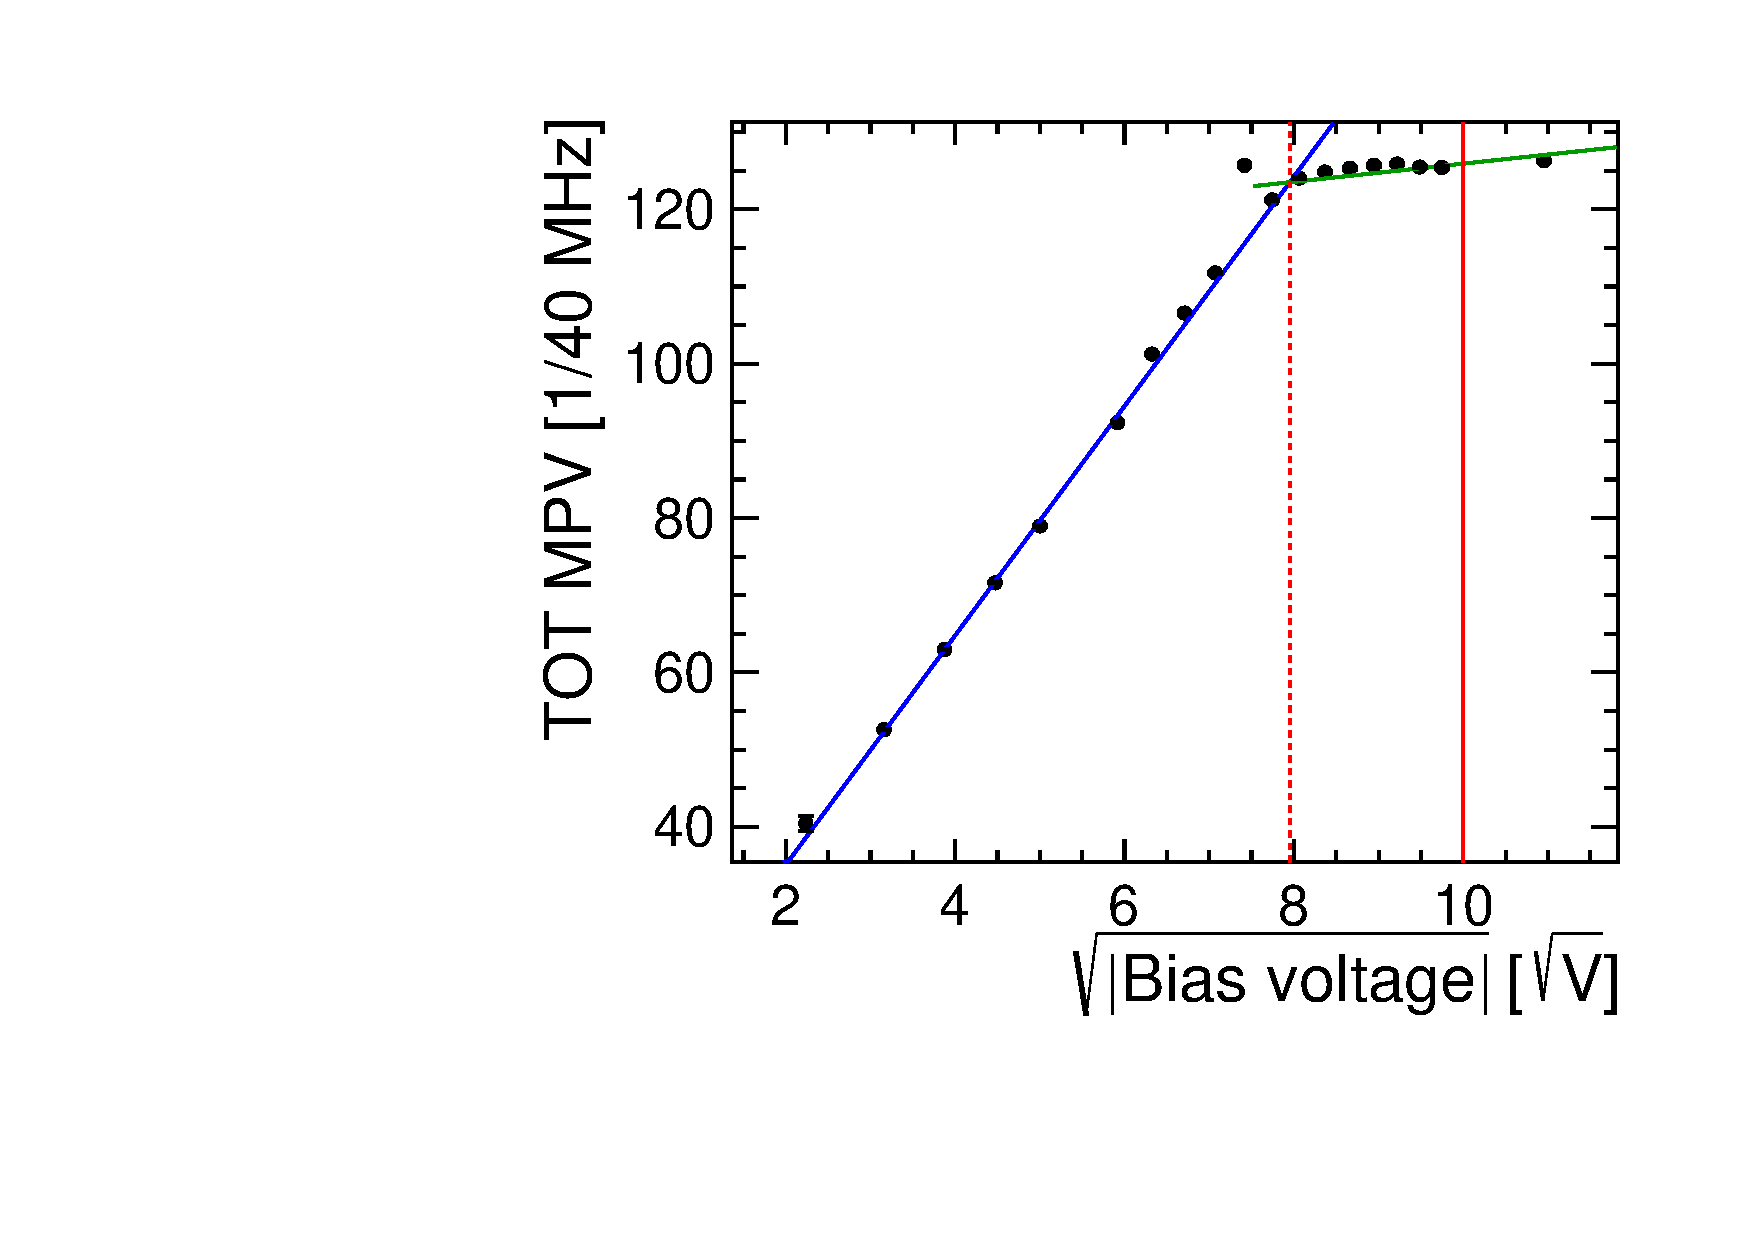
\includegraphics[width=\textwidth]{./figures/TestBeam/depletionVoltage_W0002_J05.pdf}
  %   \caption{W2\_J5}
  % \end{subfigure}
  \caption{The most probable value of the measured energy deposition as
    a function of the bias voltage for the assemblies listed in
    \cref{tab:Timepix3Assemblies}. Straight lines are used to fit the
    slope and the plateau regions. The depletion voltage corresponds
    to the intersection of these two regions and shown in a red dashed
    line. The continuous red line shows the nominal operating bias
    voltage.}
  \label{fig:depletionVoltage}
\end{figure}


%% --------------------------------------------- %%
\newpage
\section{Cluster size distribution}

The dependence of the cluster-size distribution on the bias voltage
and the operating threshold is shown for the assemblies listed in
\cref{tab:Timepix3Assemblies}.

\subsection{Cluster size distribution as a function of the bias
  voltage}

For higher bias voltages, the average cluster size decreases as shown
in \cref{fig:clusterSize_vs_biasVoltage}.

\begin{figure}[htbp] \centering
  \begin{subfigure}[b]{0.33\textwidth}
    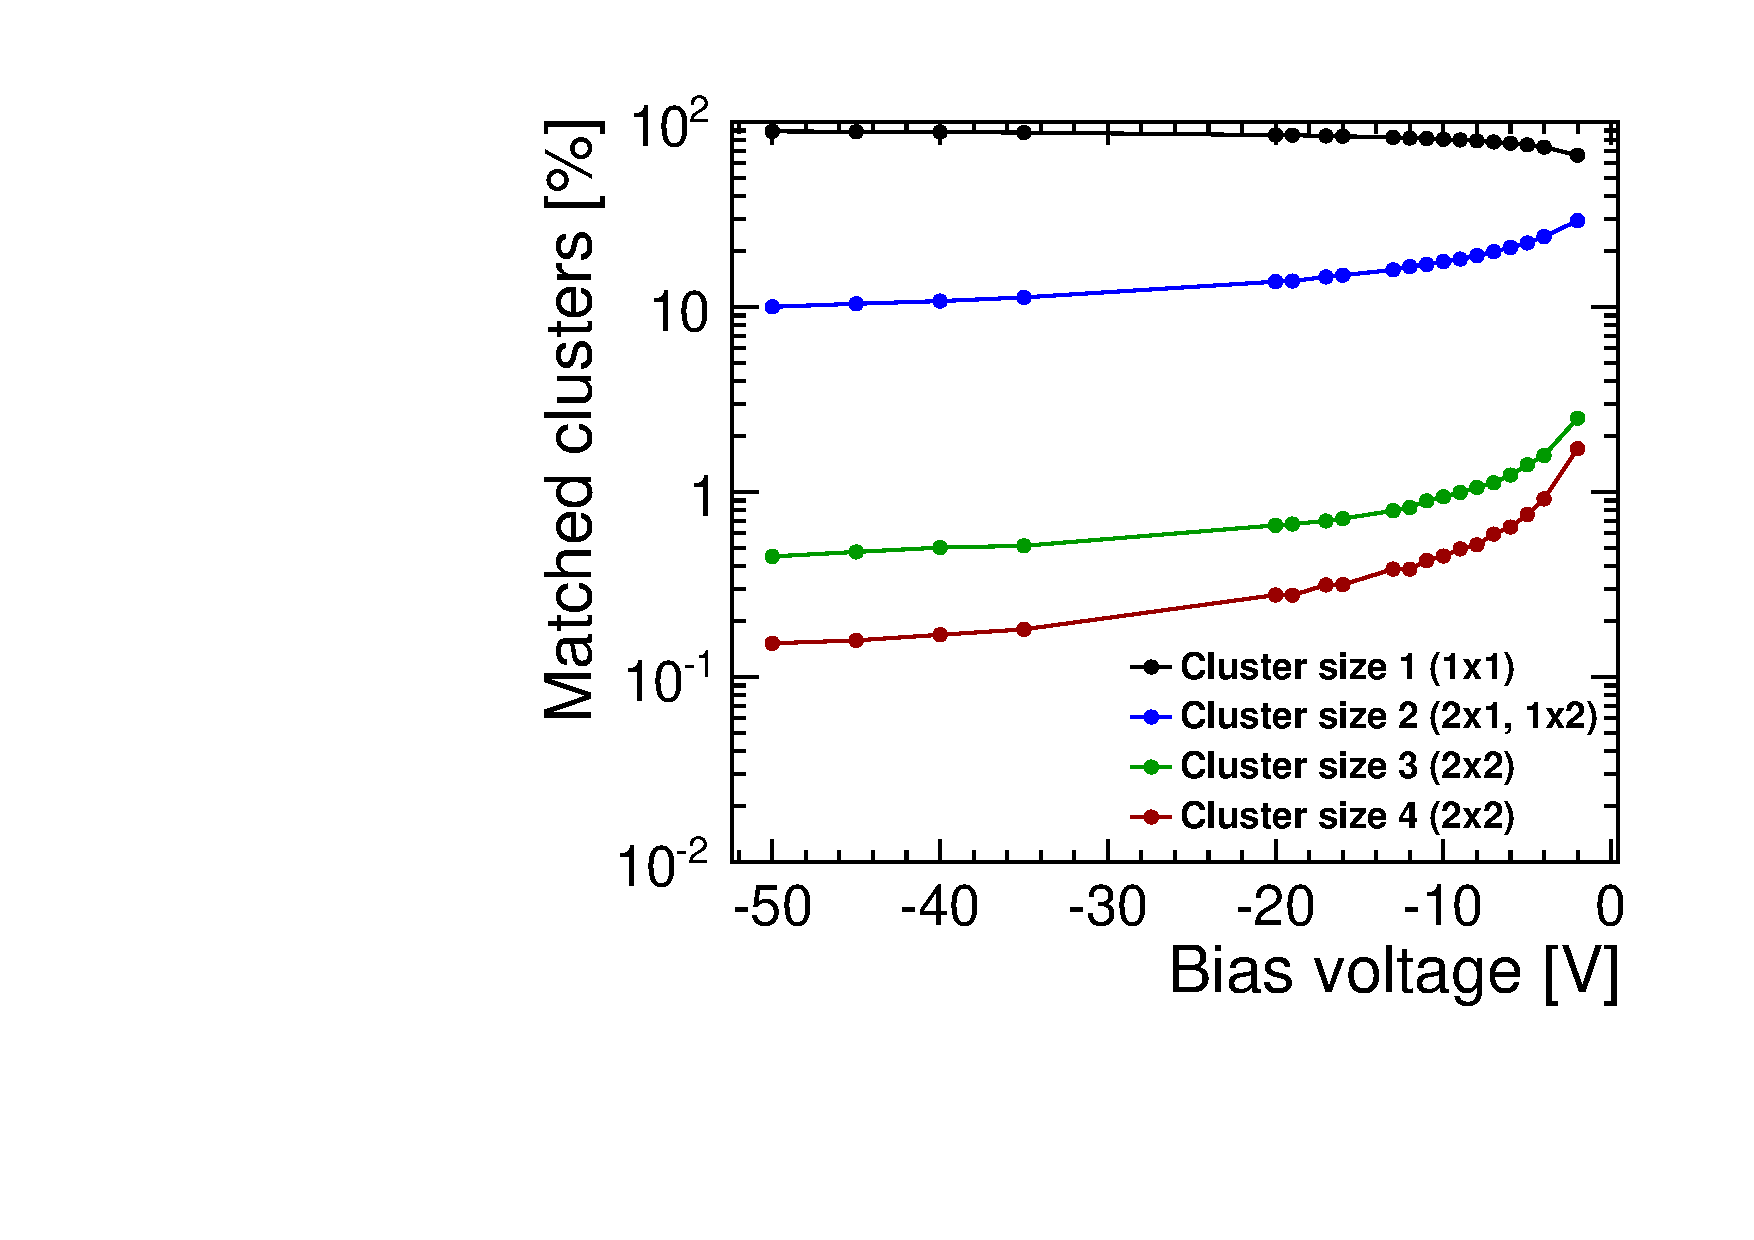
\includegraphics[width=\textwidth]{./figures/TestBeam/cluSize_biasScan_W0019_G07.pdf}
    \caption{W19\_G7}
  \end{subfigure} \hfill
  \begin{subfigure}[b]{0.33\textwidth}
    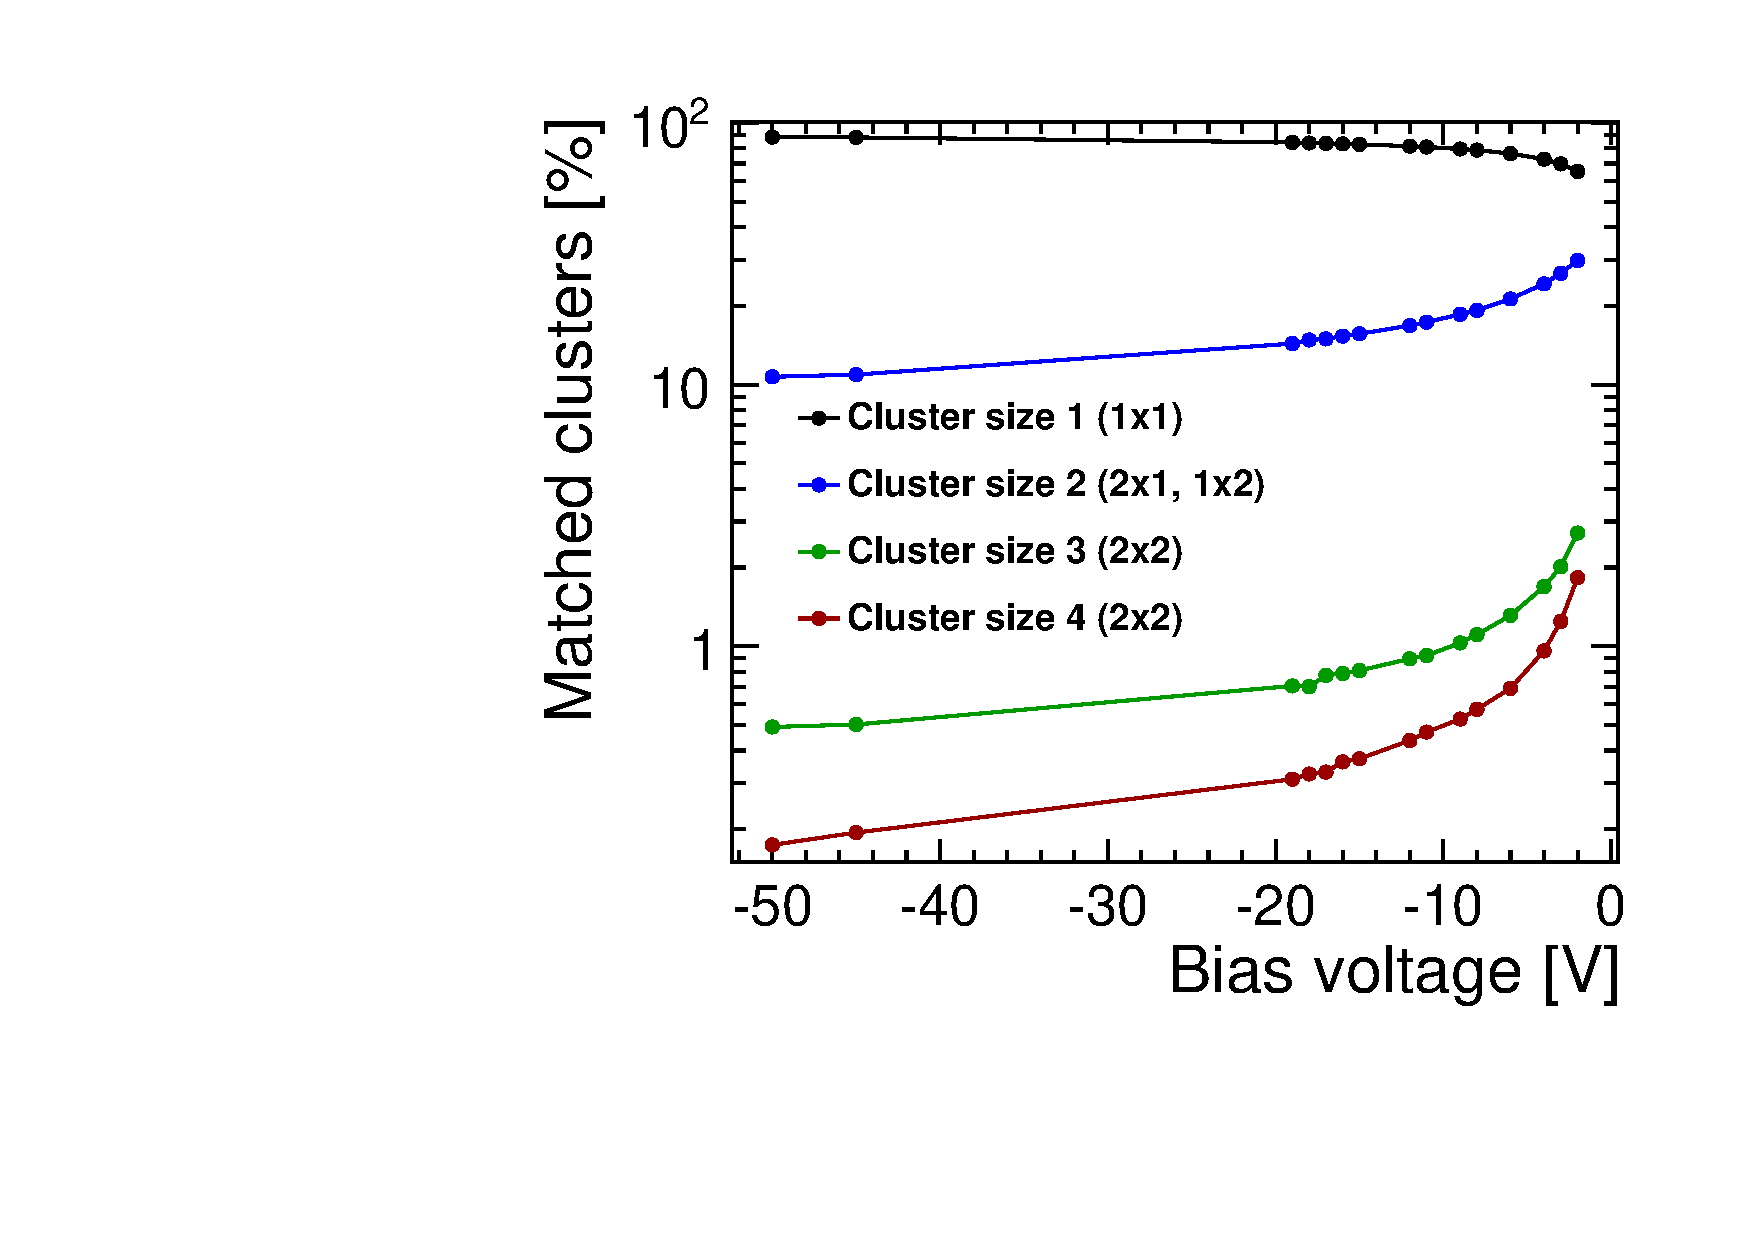
\includegraphics[width=\textwidth]{./figures/TestBeam/cluSize_biasScan_W0019_F07.pdf}
    \caption{W19\_F7}
  \end{subfigure}\hfill
  \begin{subfigure}[b]{0.33\textwidth}
    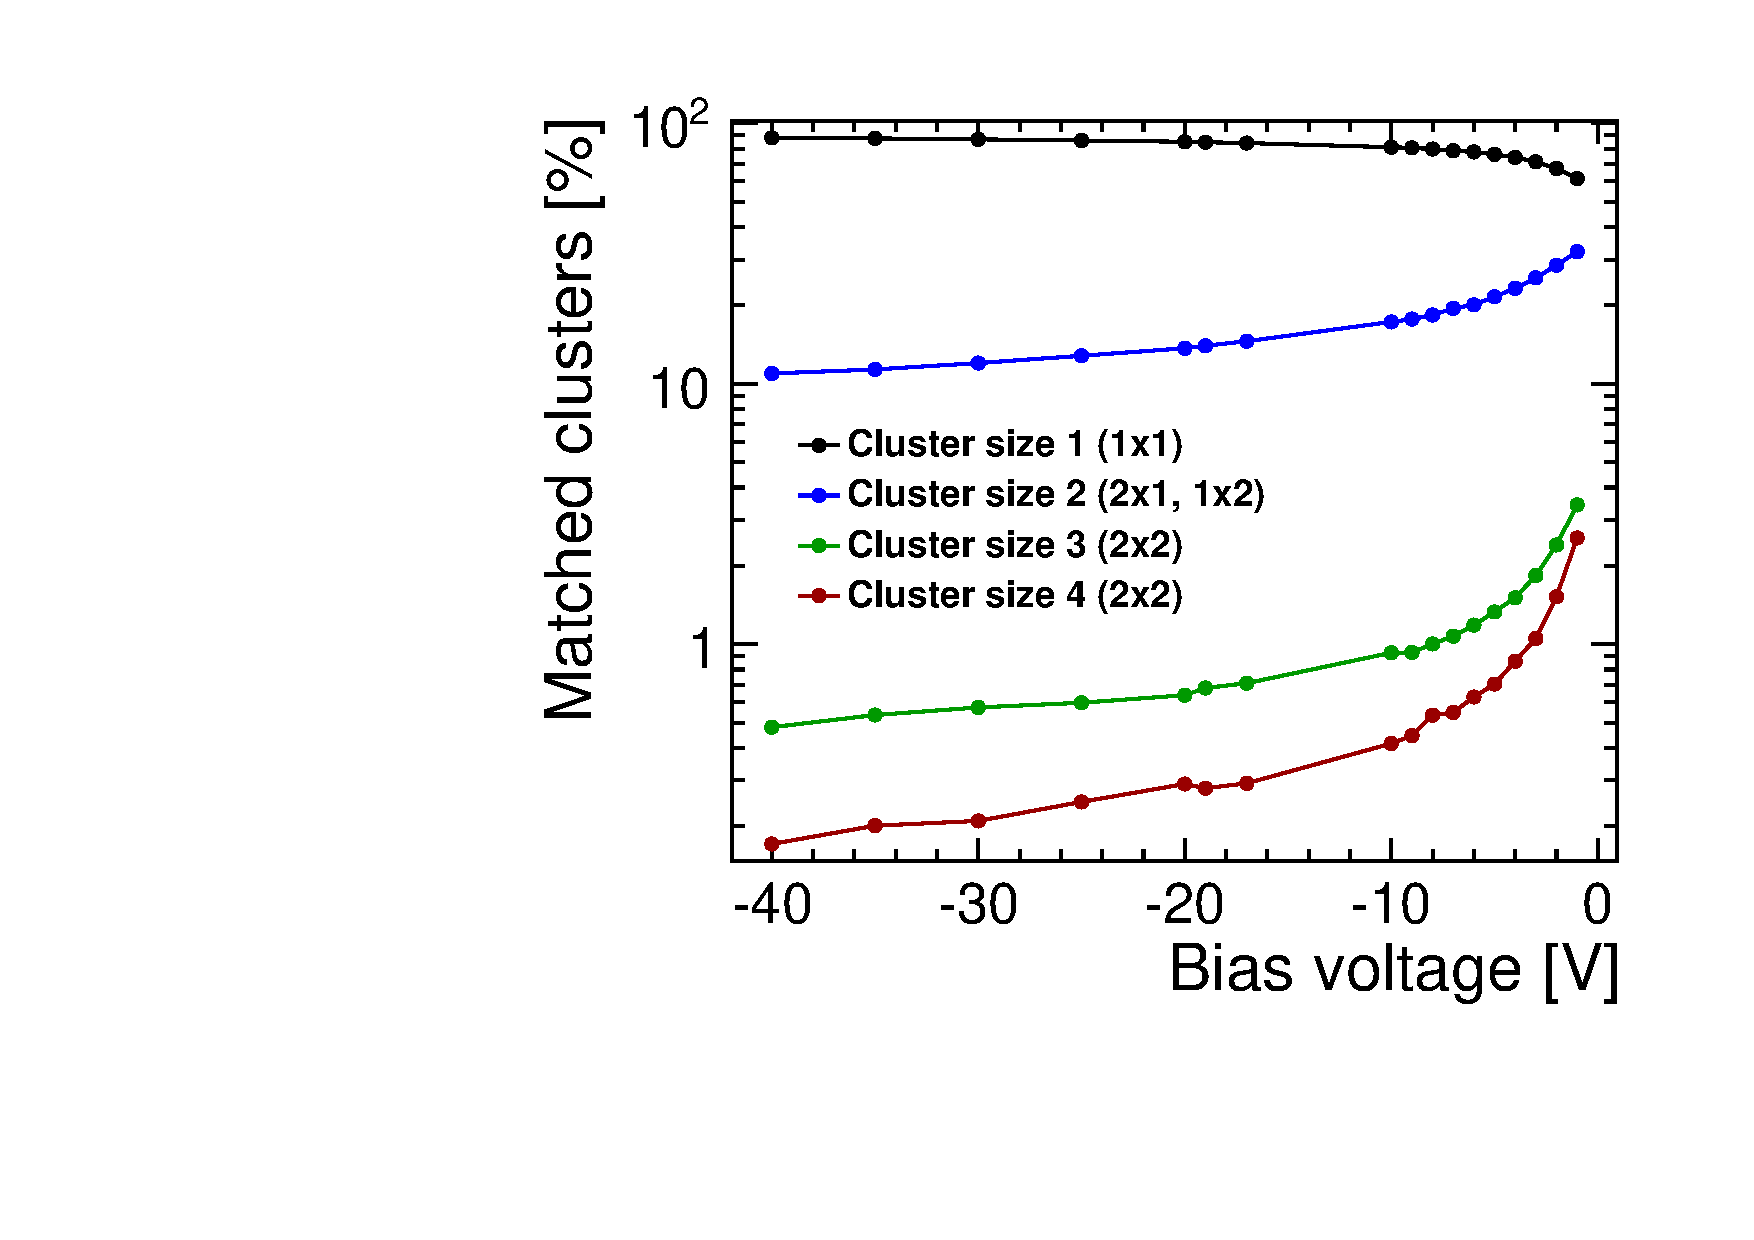
\includegraphics[width=\textwidth]{./figures/TestBeam/cluSize_biasScan_W0019_L08.pdf}
    \caption{W19\_L8}
  \end{subfigure} \\

  \begin{subfigure}[b]{0.33\textwidth}
    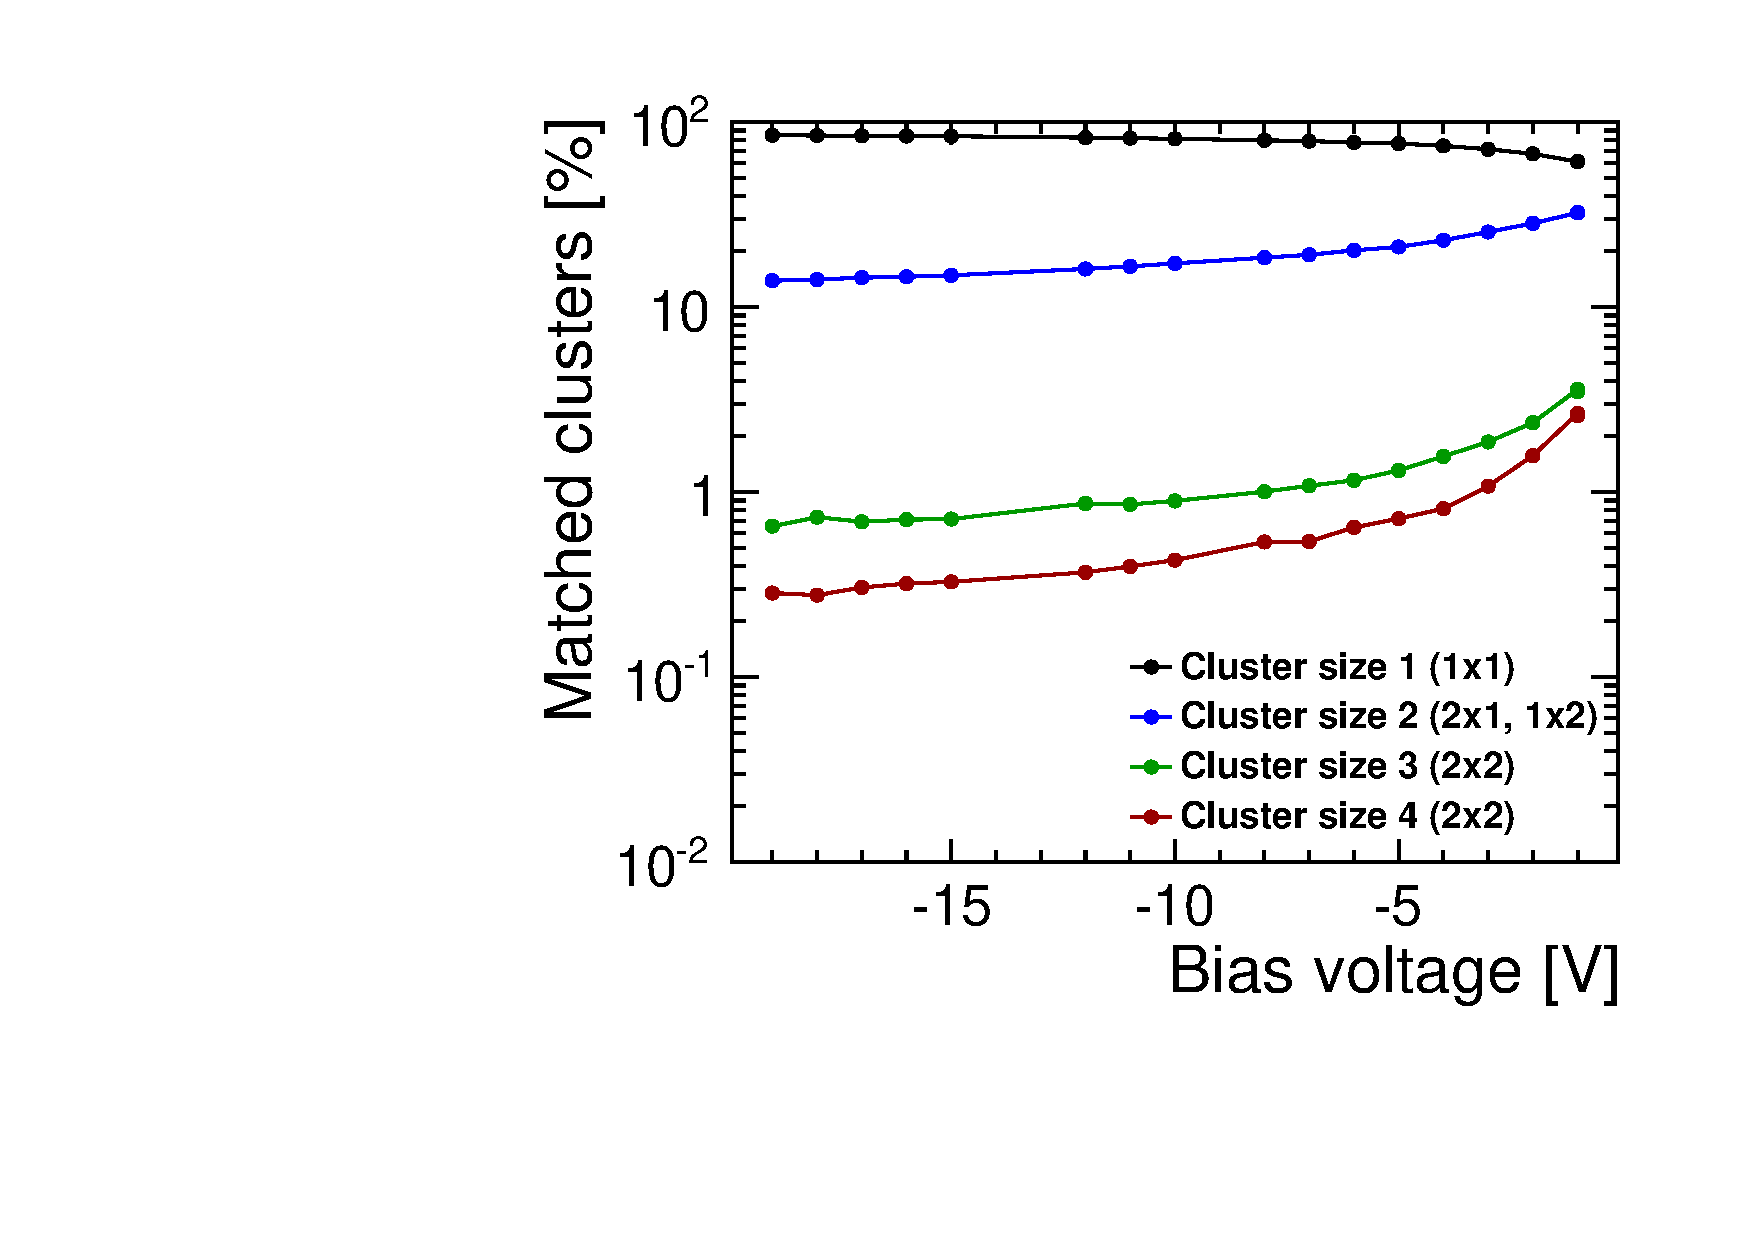
\includegraphics[width=\textwidth]{./figures/TestBeam/cluSize_biasScan_W0019_C07.pdf}
    \caption{W19\_C7}
  \end{subfigure} \hfill
  \begin{subfigure}[b]{0.33\textwidth}
    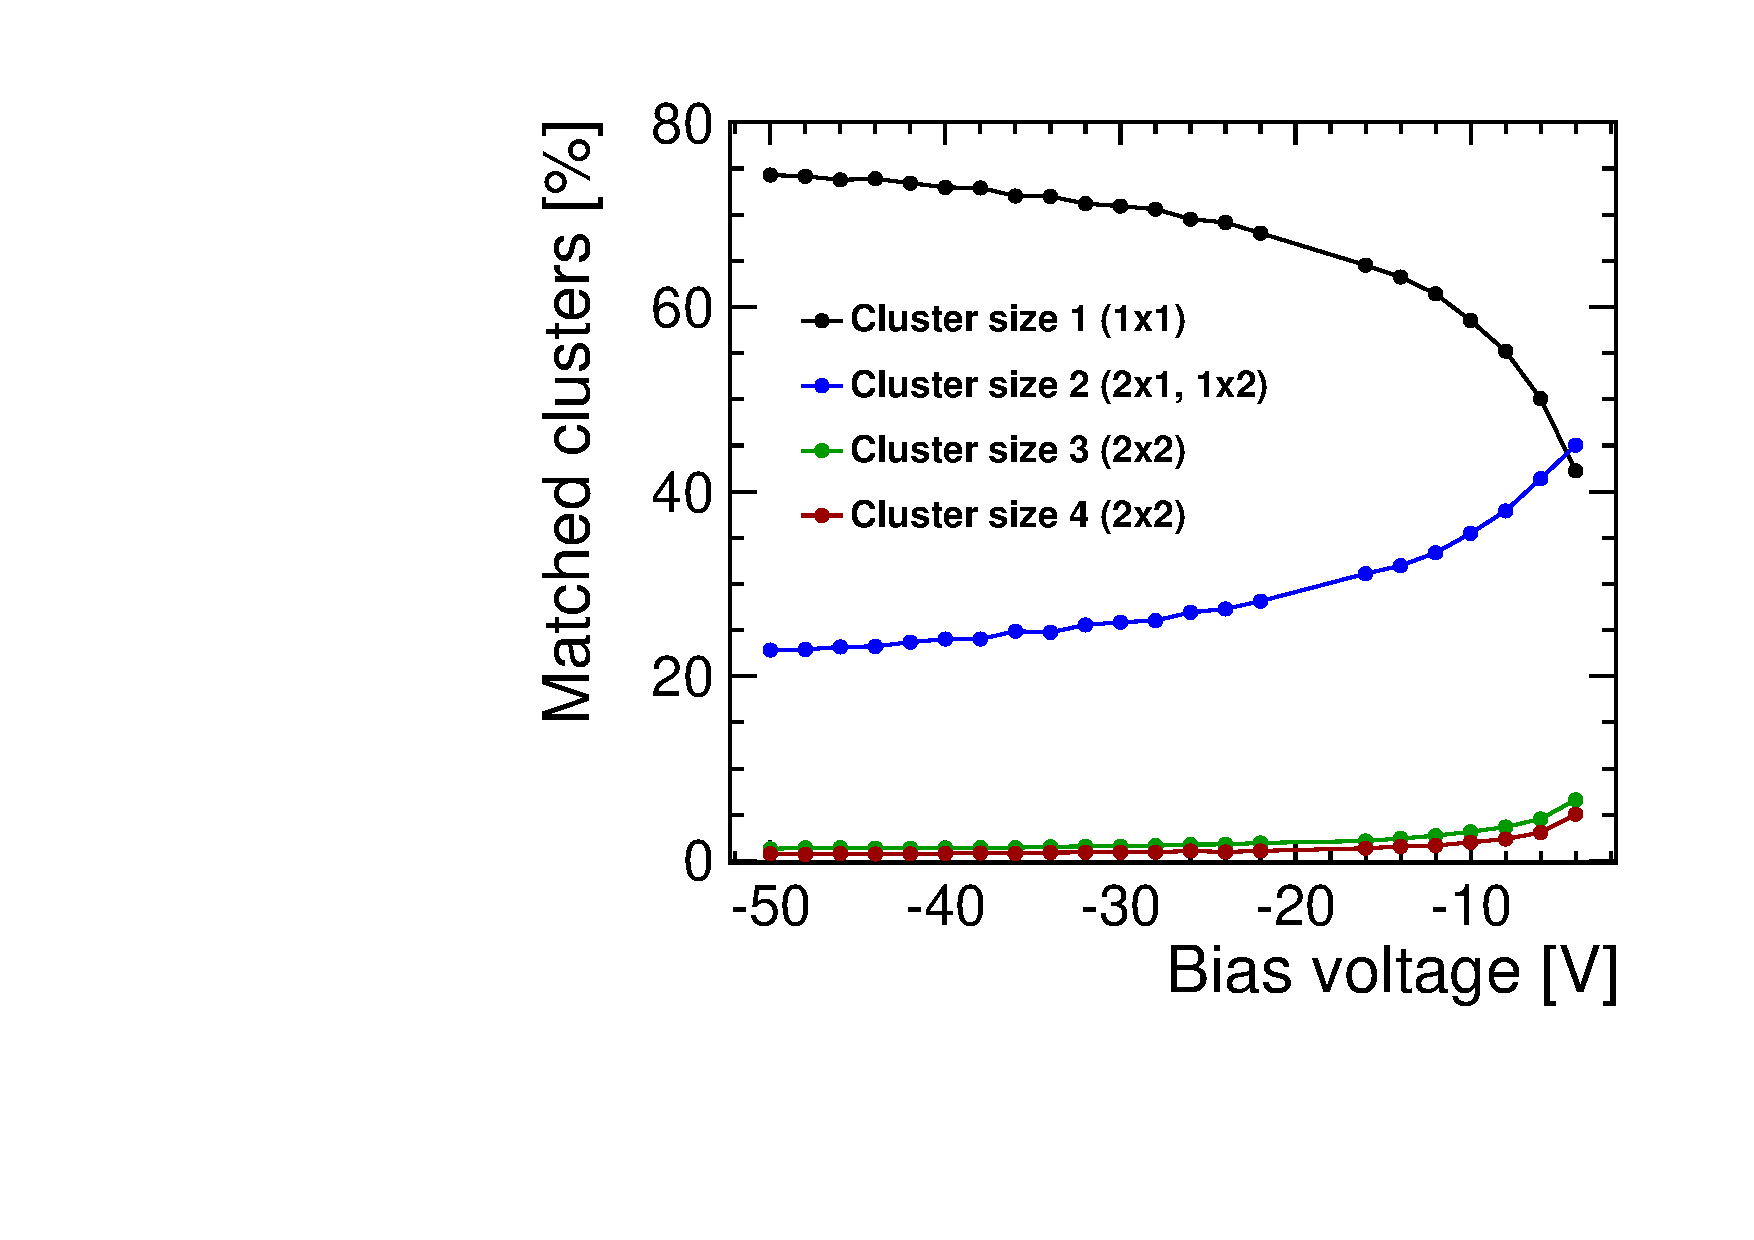
\includegraphics[width=\textwidth]{./figures/TestBeam/cluSize_biasScan_W0005_E02.pdf}
    \caption{W5\_E2}
  \end{subfigure}\hfill
  \begin{subfigure}[b]{0.33\textwidth}
    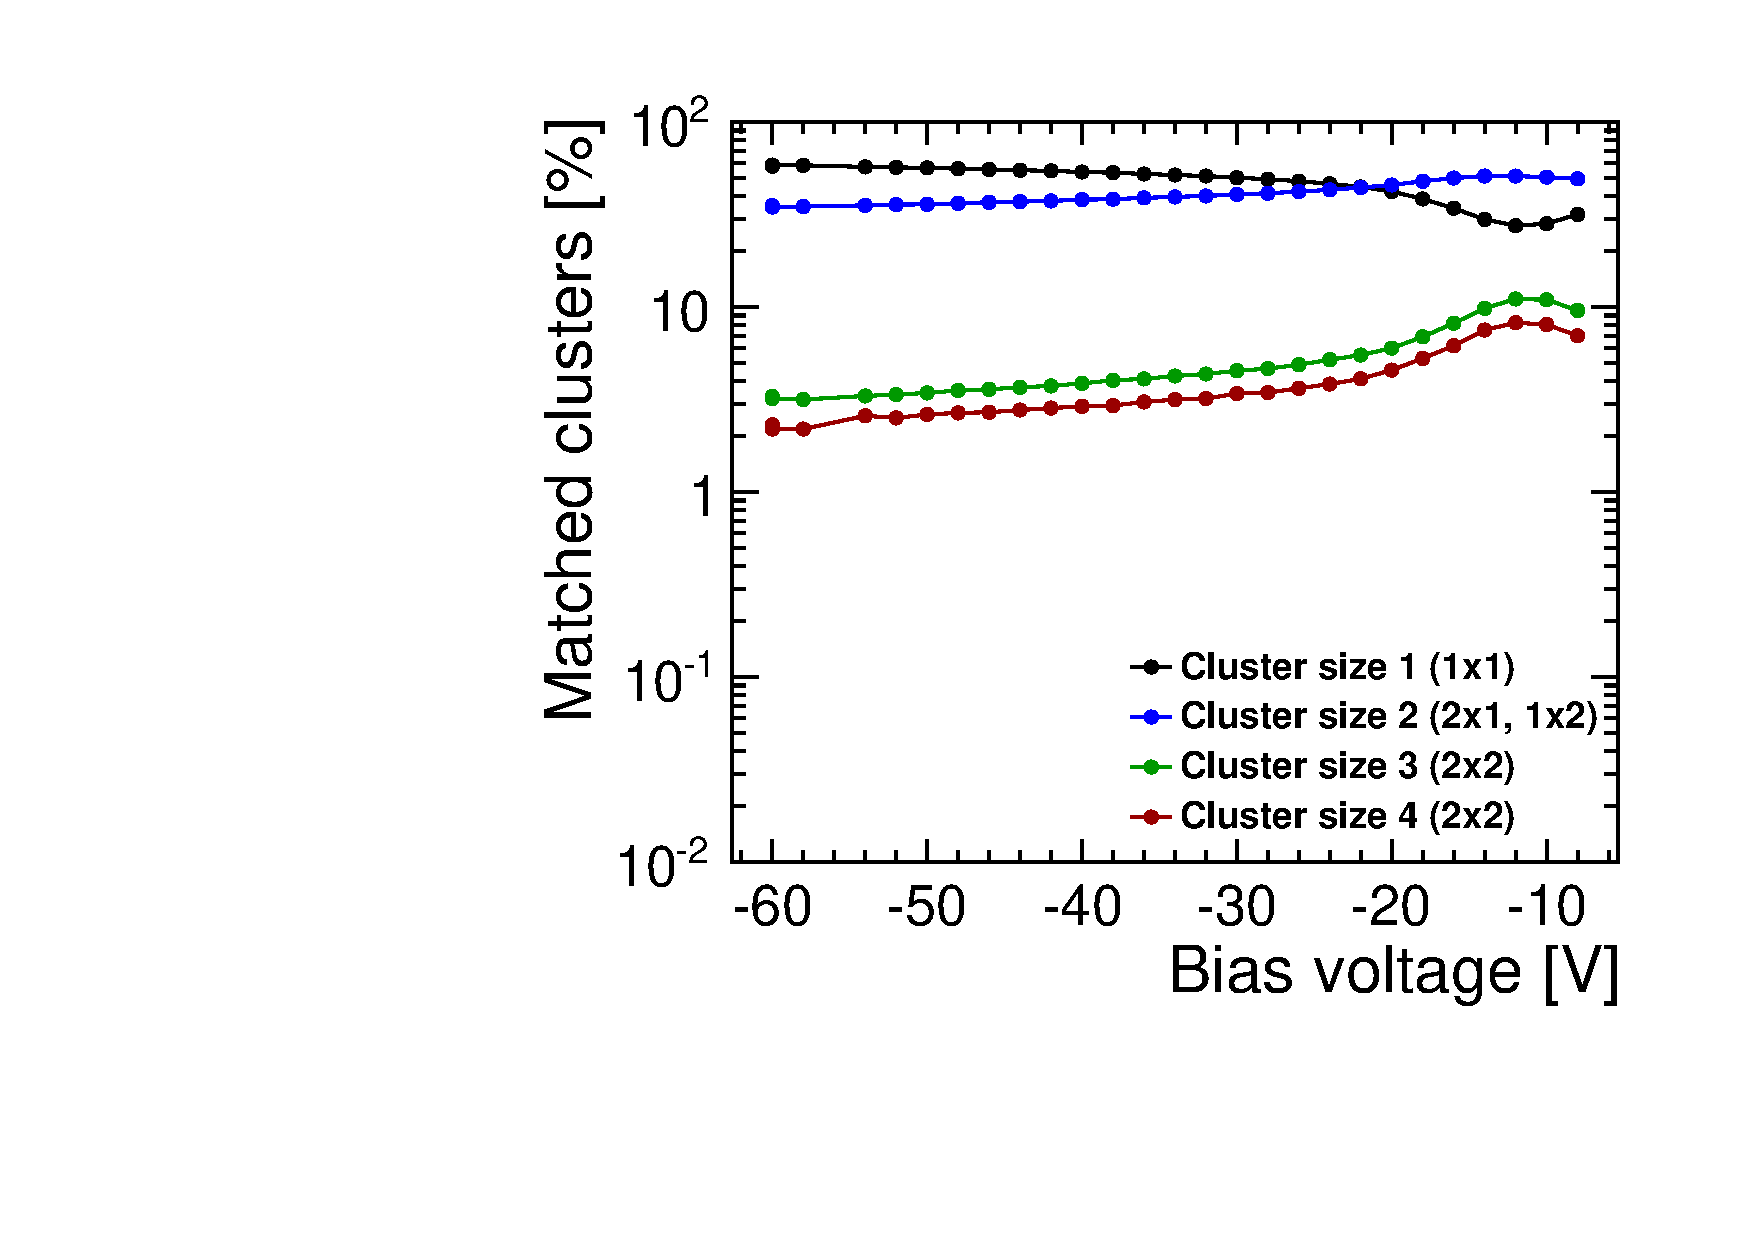
\includegraphics[width=\textwidth]{./figures/TestBeam/cluSize_biasScan_W0005_F01.pdf}
    \caption{W5\_F1}
  \end{subfigure}%\\
  % \begin{subfigure}[b]{0.33\textwidth}
  %   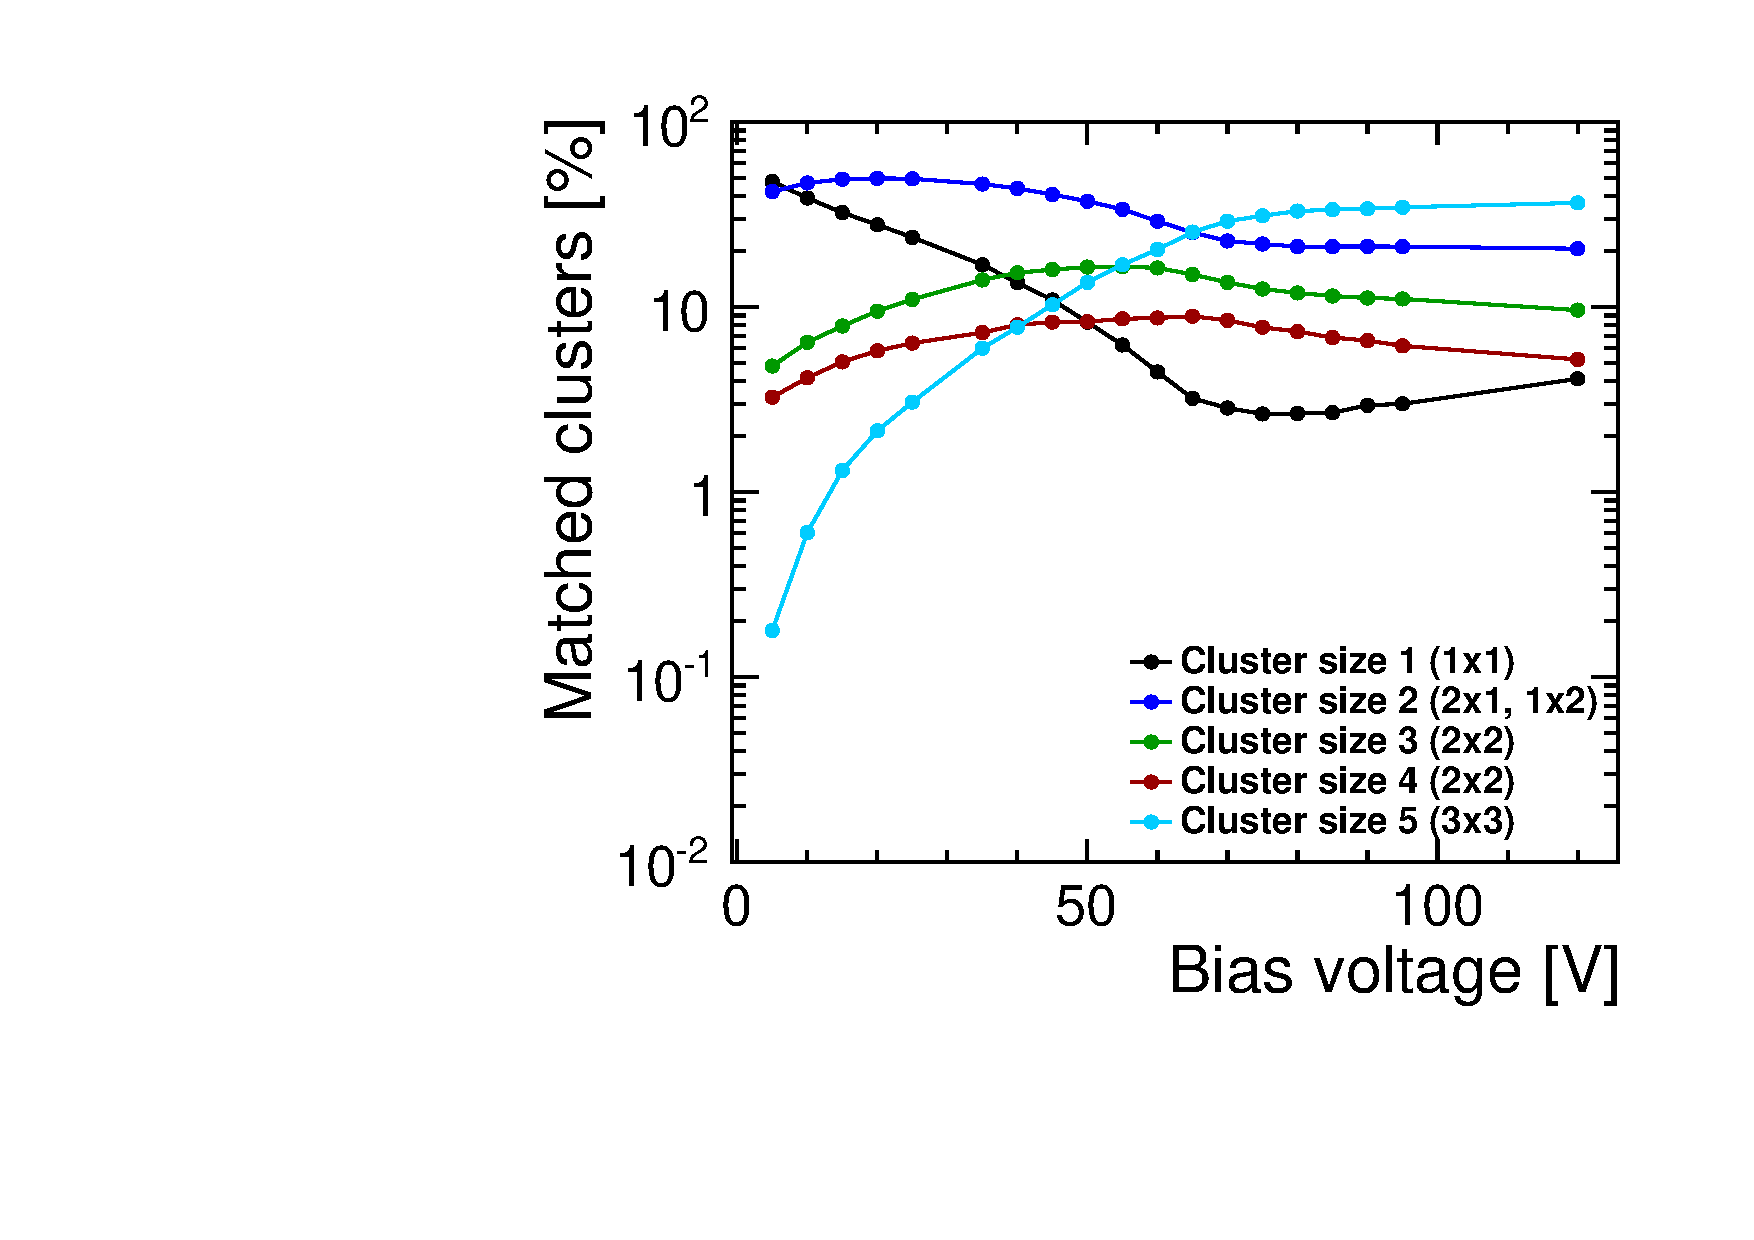
\includegraphics[width=\textwidth]{./figures/TestBeam/cluSize_biasScan_W0002_J05.pdf}
  %   \caption{W2\_J5}
  % \end{subfigure}
  \caption{Cluster size distribution as a function of the applied
    voltage for assemblies listed in \cref{tab:Timepix3Assemblies}.}
  \label{fig:clusterSize_vs_biasVoltage}
\end{figure}

\subsection{Cluster size distribution as a function of the operating
  threshold}

Lowering the threshold leads to an increase in the average cluster
size fraction distribution as shown in
\cref{fig:clusterSize_vs_THLscan}.

\begin{figure}[htbp] \centering
  \begin{subfigure}[b]{0.33\textwidth}
    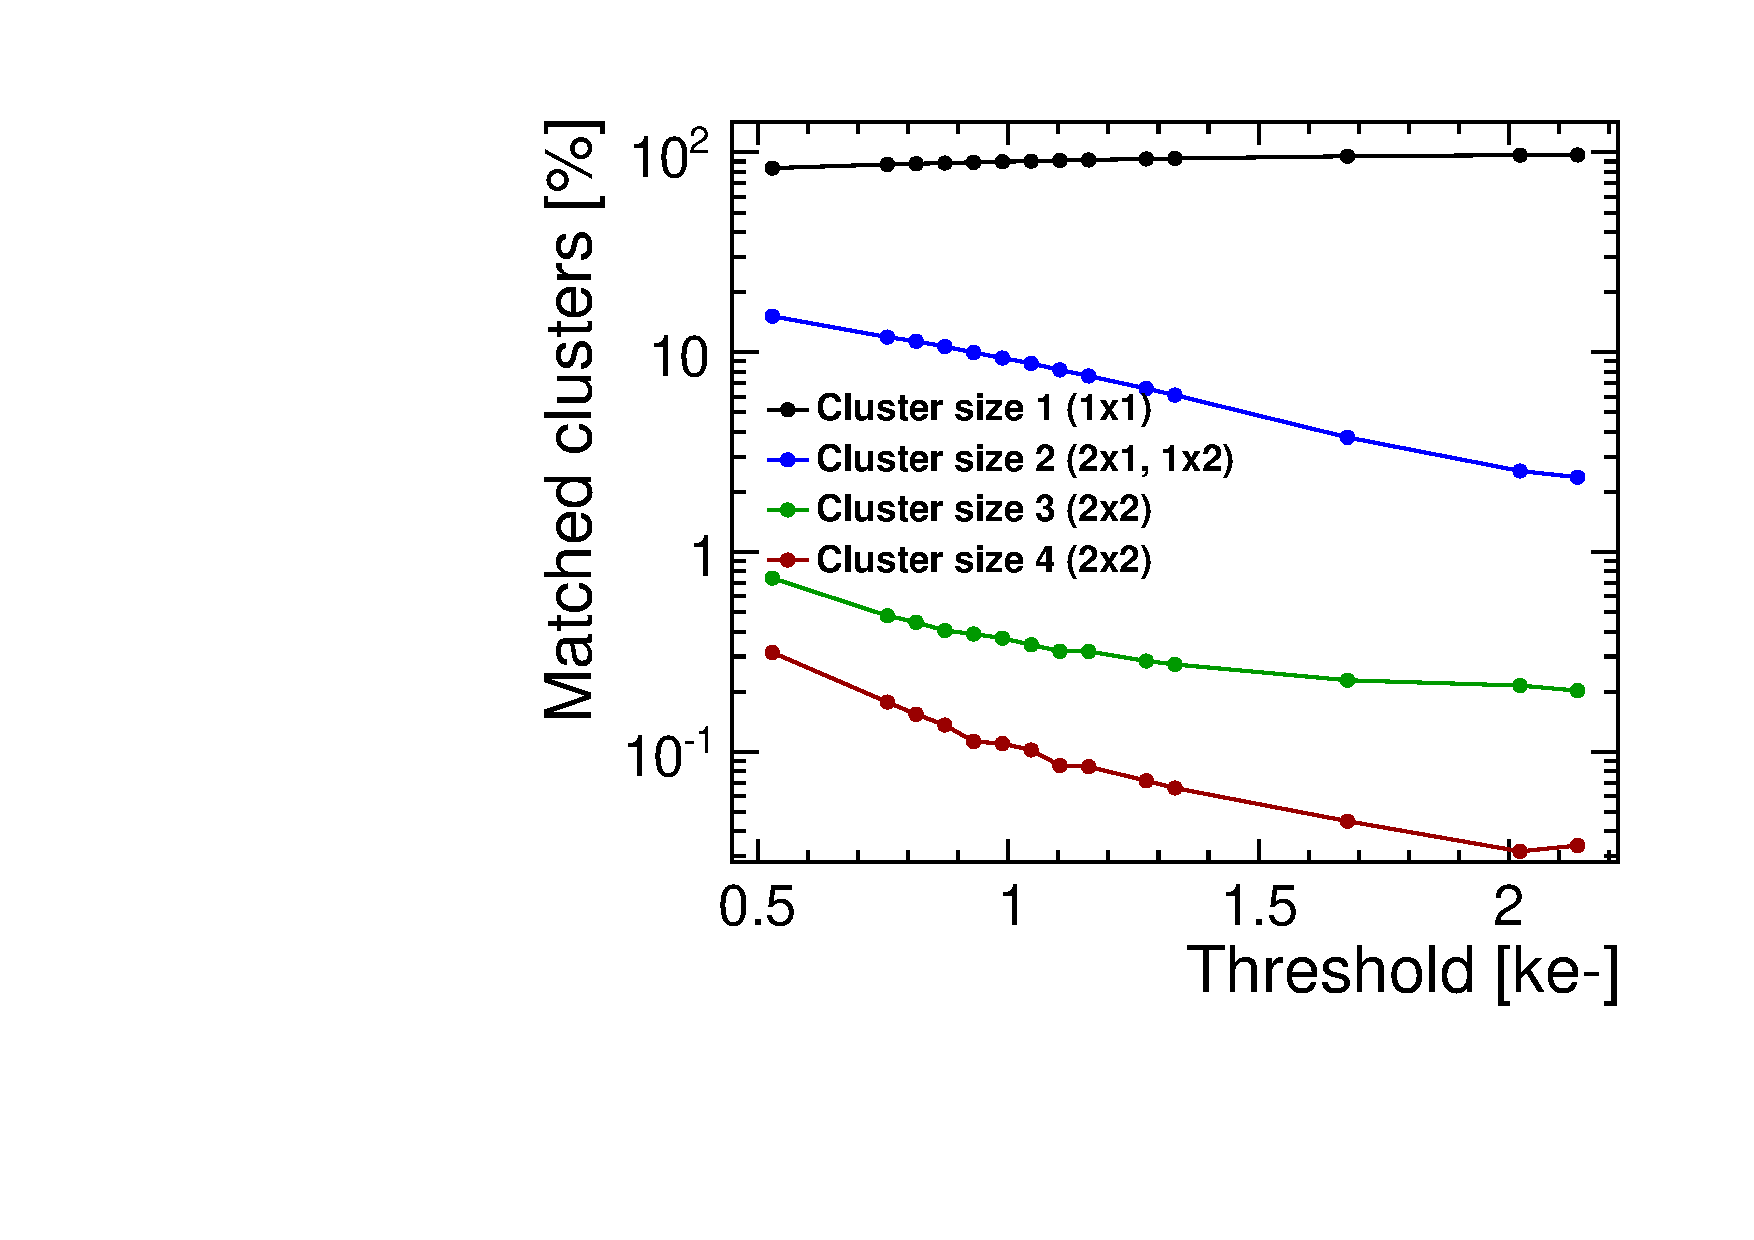
\includegraphics[width=\textwidth]{./figures/TestBeam/cluSize_THLscan_W0019_G07.pdf}
    \caption{W19\_G7}
  \end{subfigure} \hfill
  \begin{subfigure}[b]{0.33\textwidth}
    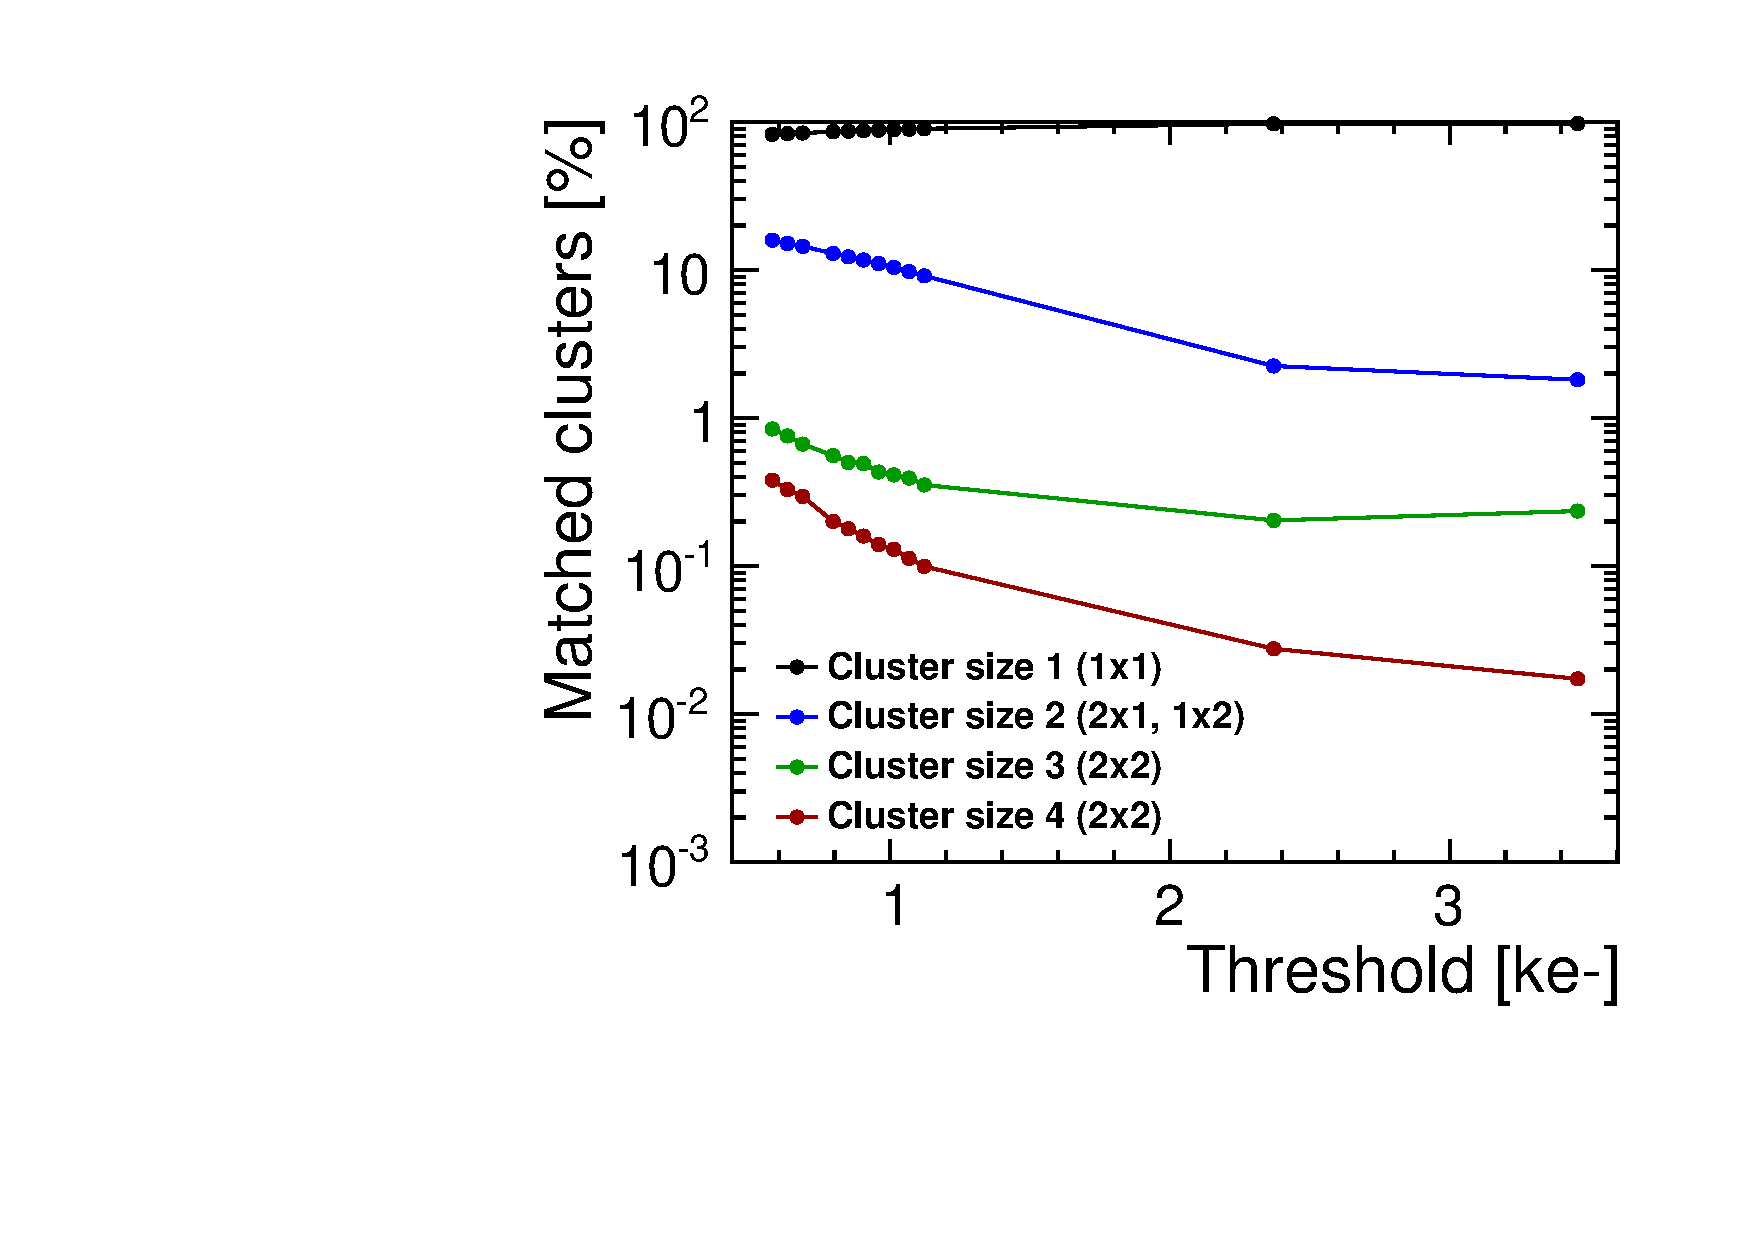
\includegraphics[width=\textwidth]{./figures/TestBeam/cluSize_THLscan_W0019_F07.pdf}
    \caption{W19\_F7}
  \end{subfigure}\hfill
  \begin{subfigure}[b]{0.33\textwidth}
    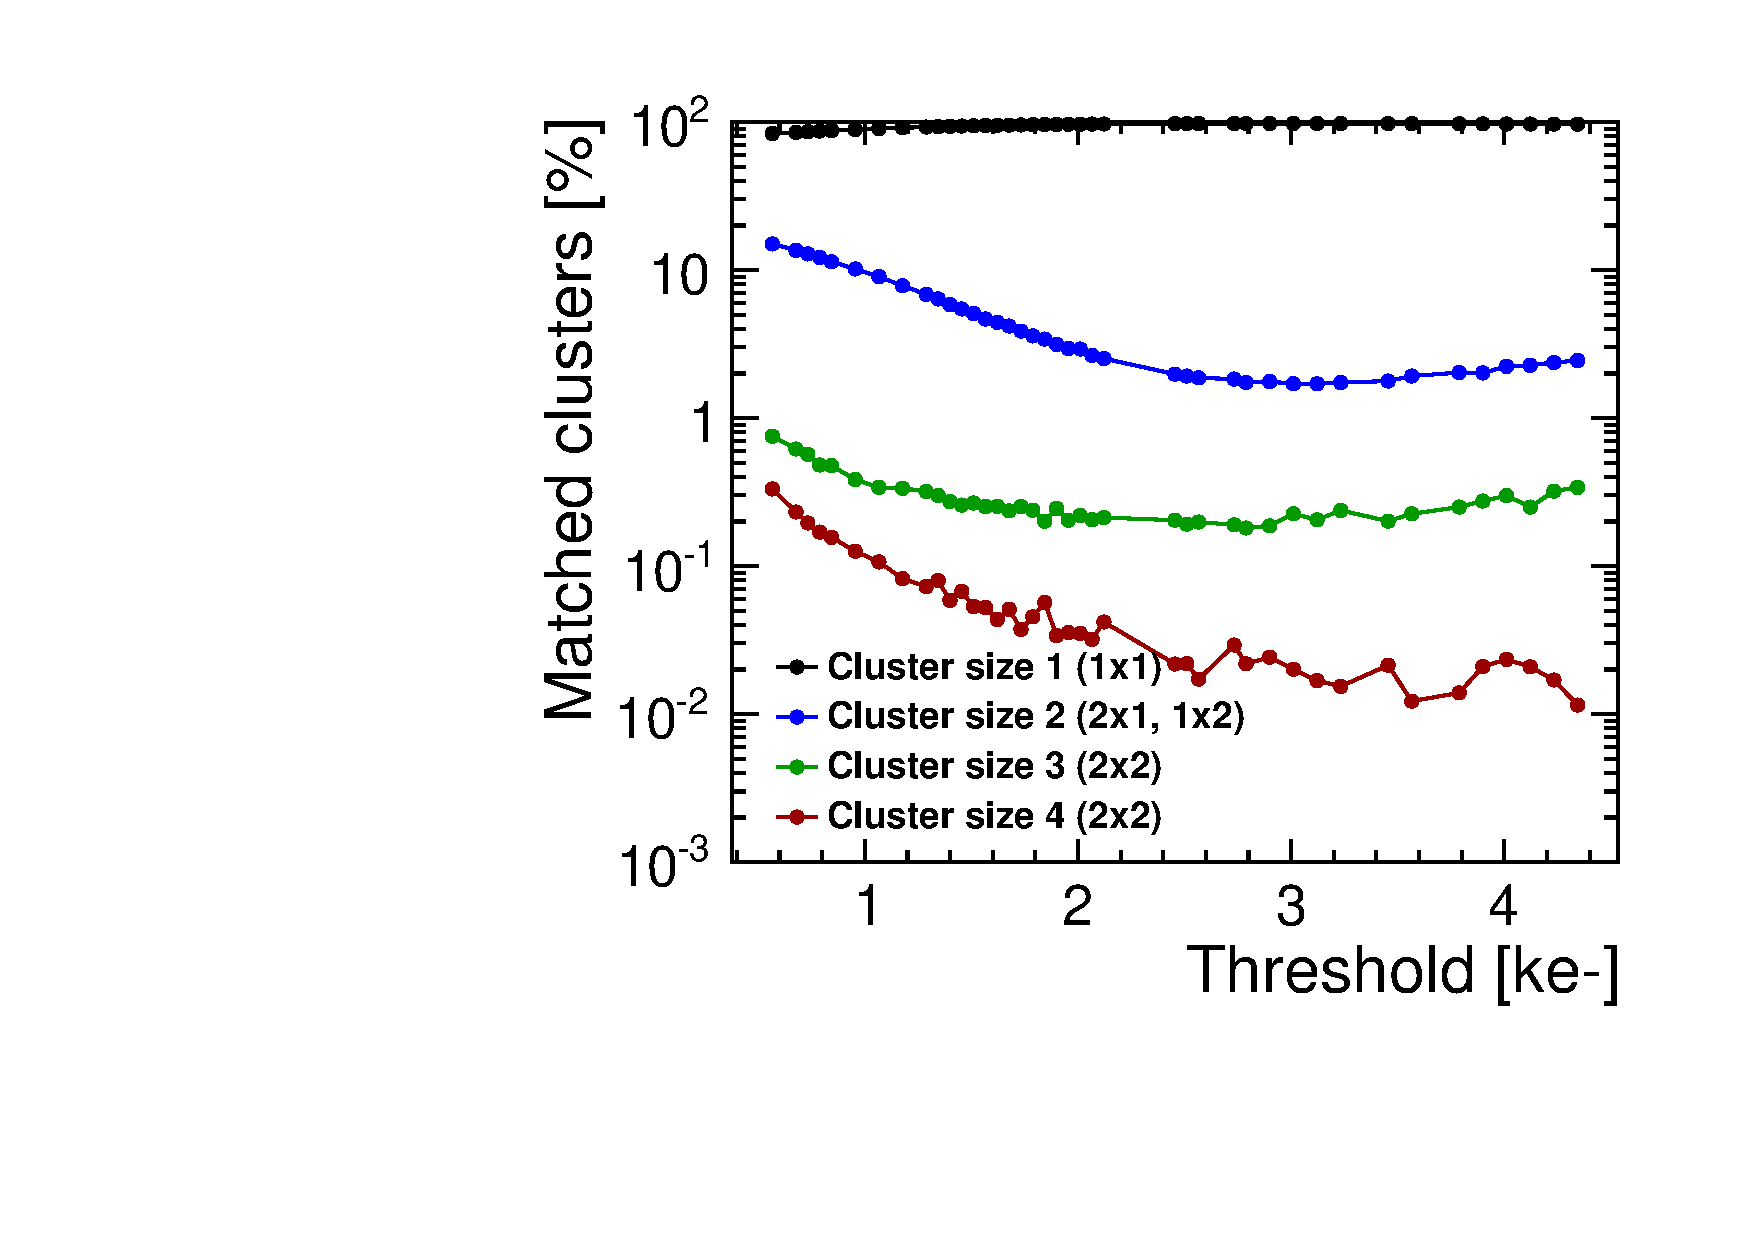
\includegraphics[width=\textwidth]{./figures/TestBeam/cluSize_THLscan_W0019_L08.pdf}
    \caption{W19\_L8}
  \end{subfigure} \\

  \begin{subfigure}[b]{0.33\textwidth}
    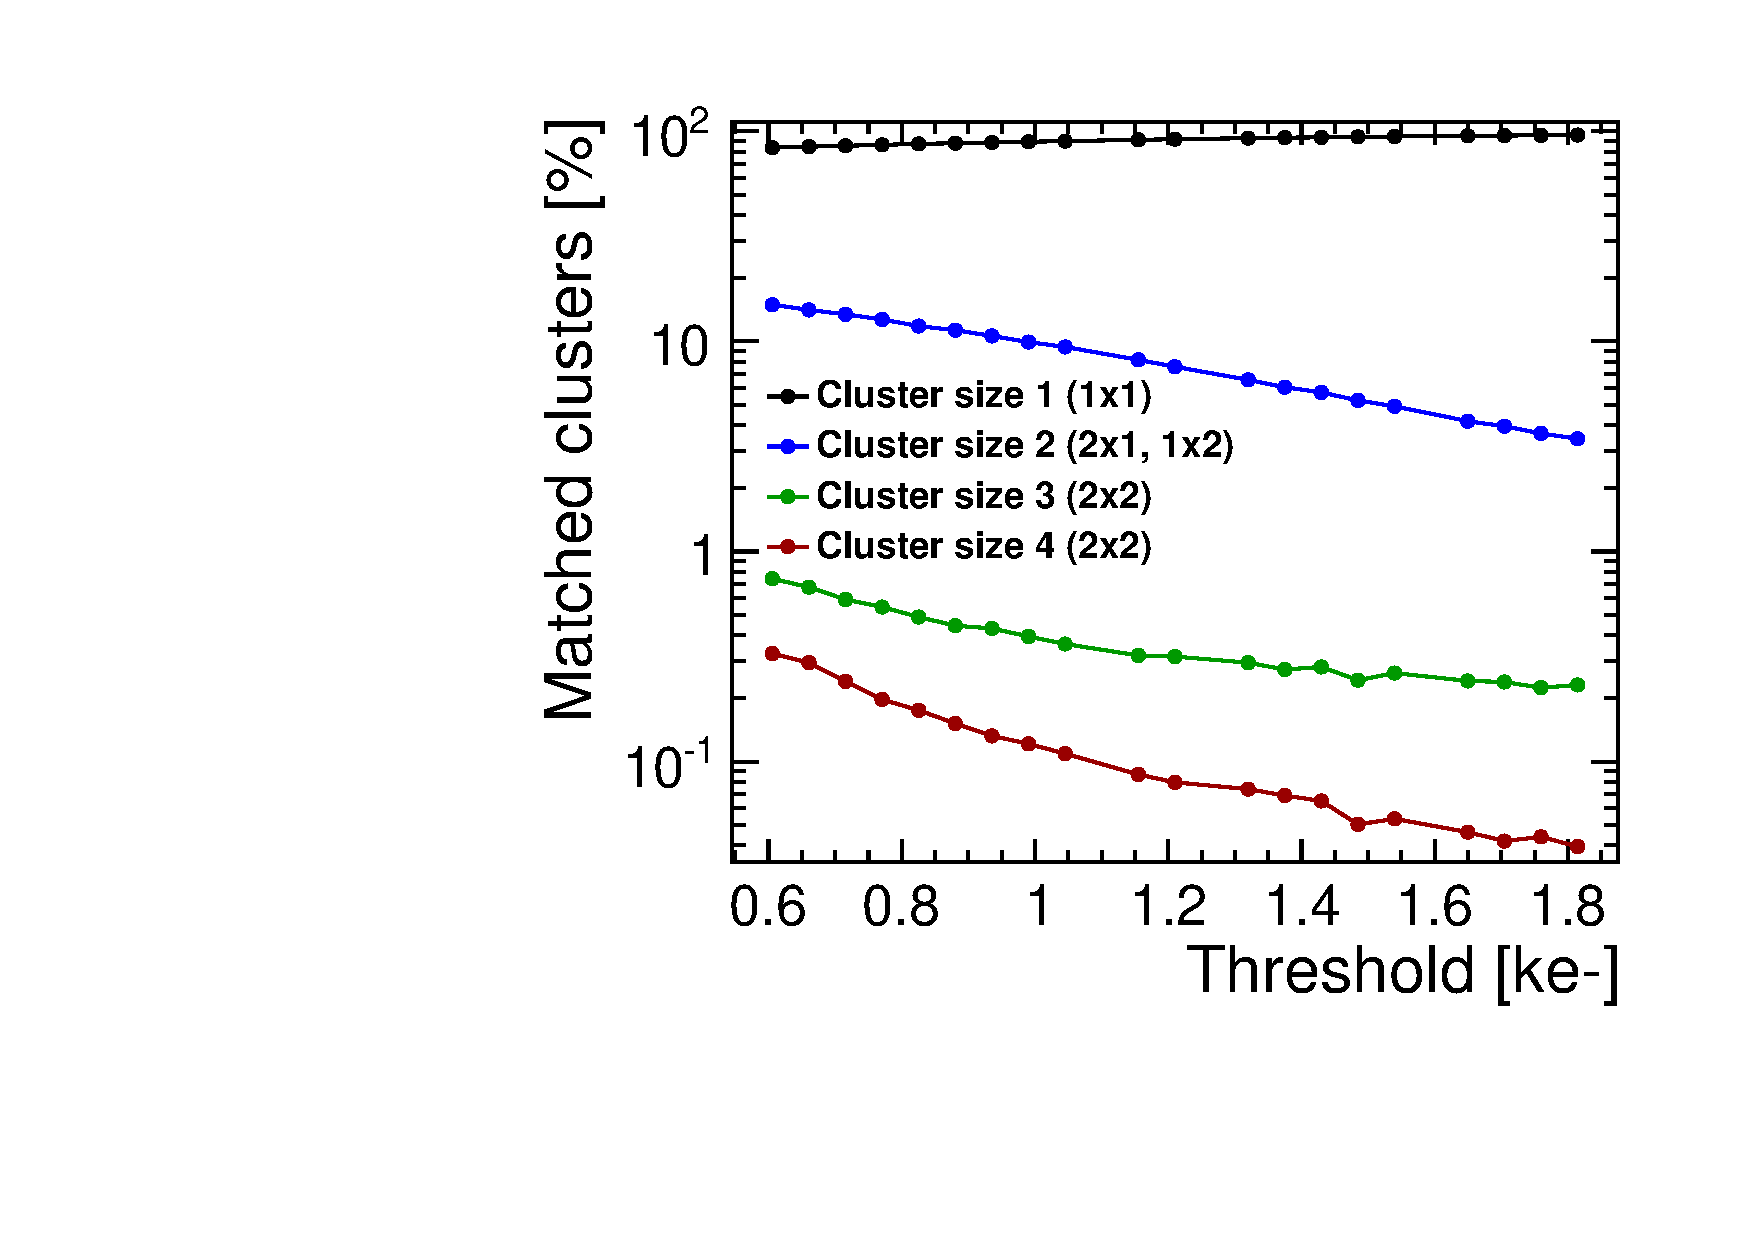
\includegraphics[width=\textwidth]{./figures/TestBeam/cluSize_THLscan_W0019_C07.pdf}
    \caption{W19\_C7}
  \end{subfigure} \hfill
  \begin{subfigure}[b]{0.33\textwidth}
    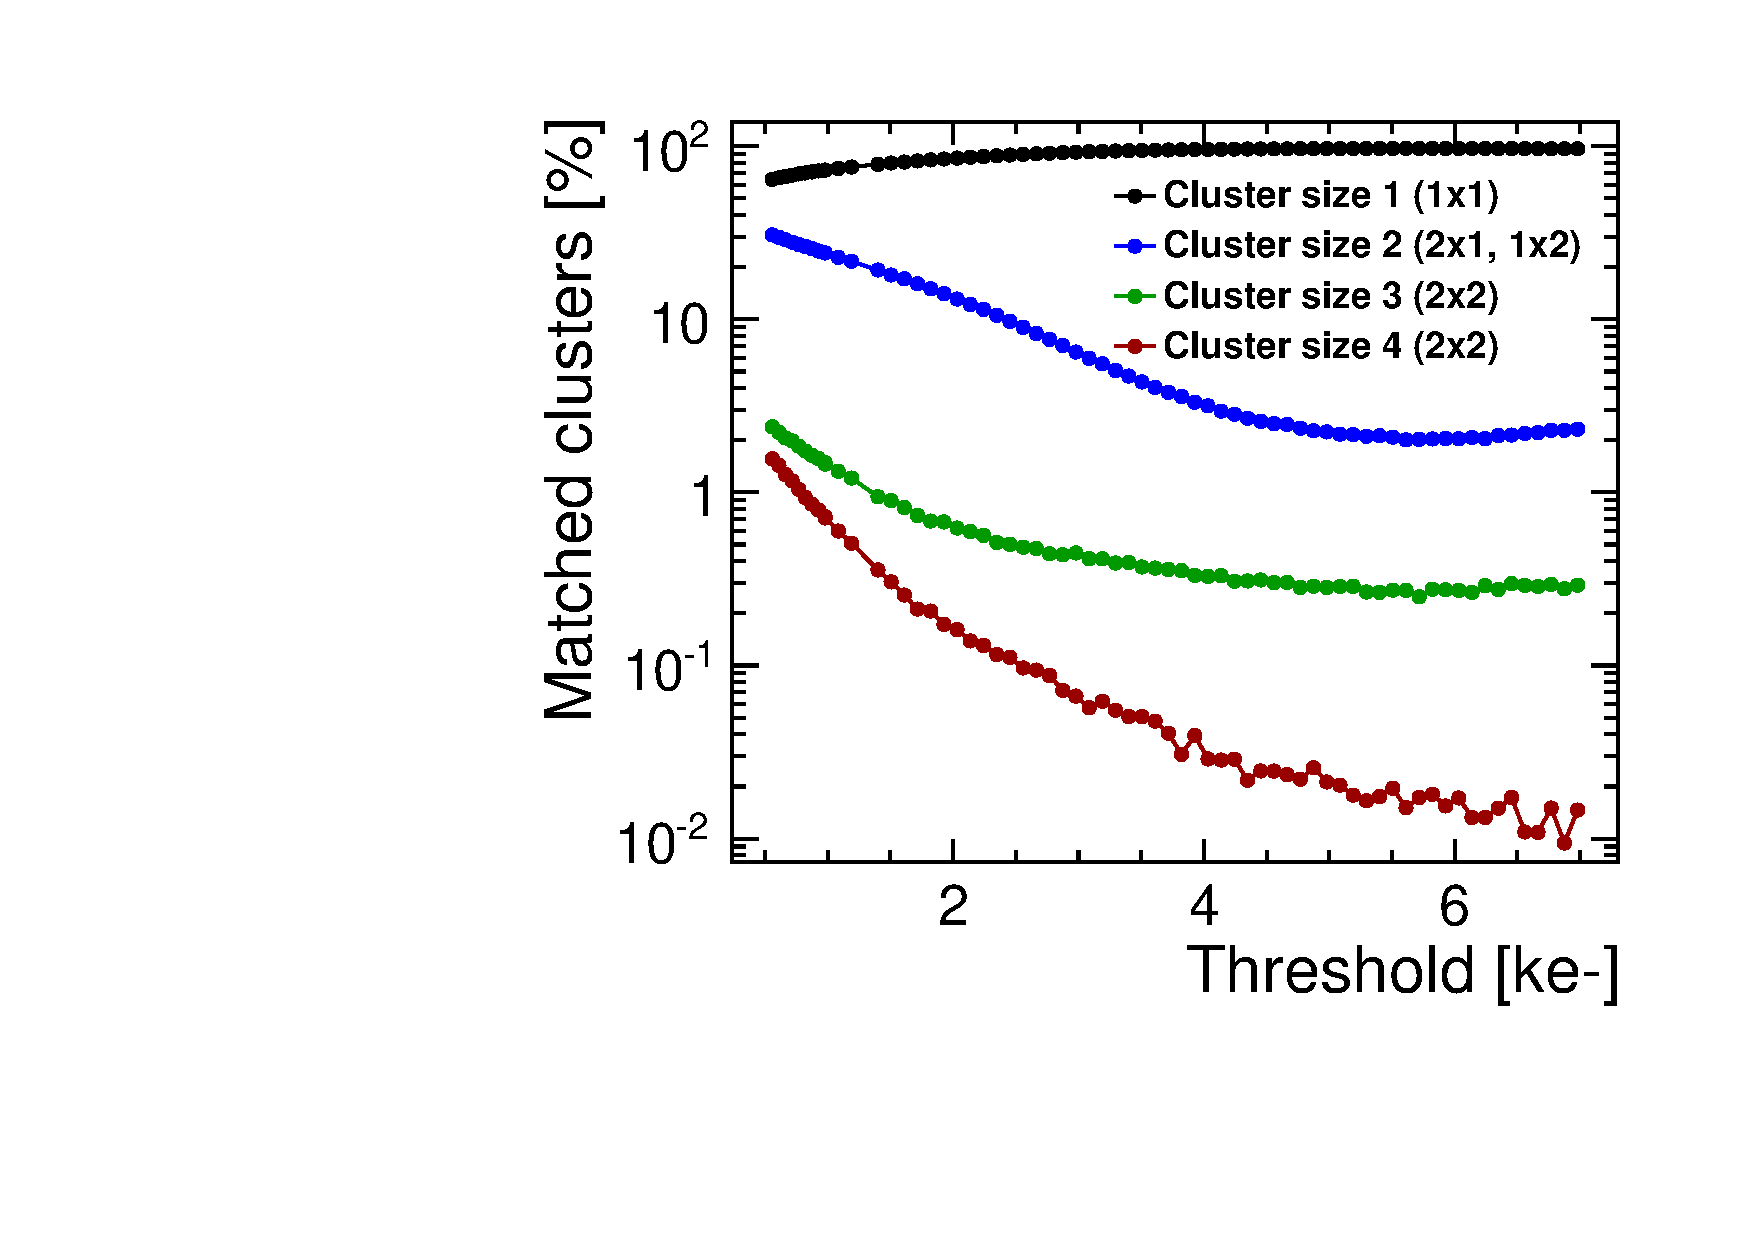
\includegraphics[width=\textwidth]{./figures/TestBeam/cluSize_THLscan_W0005_E02.pdf}
    \caption{W5\_E2}
  \end{subfigure}\hfill
  \begin{subfigure}[b]{0.33\textwidth}
    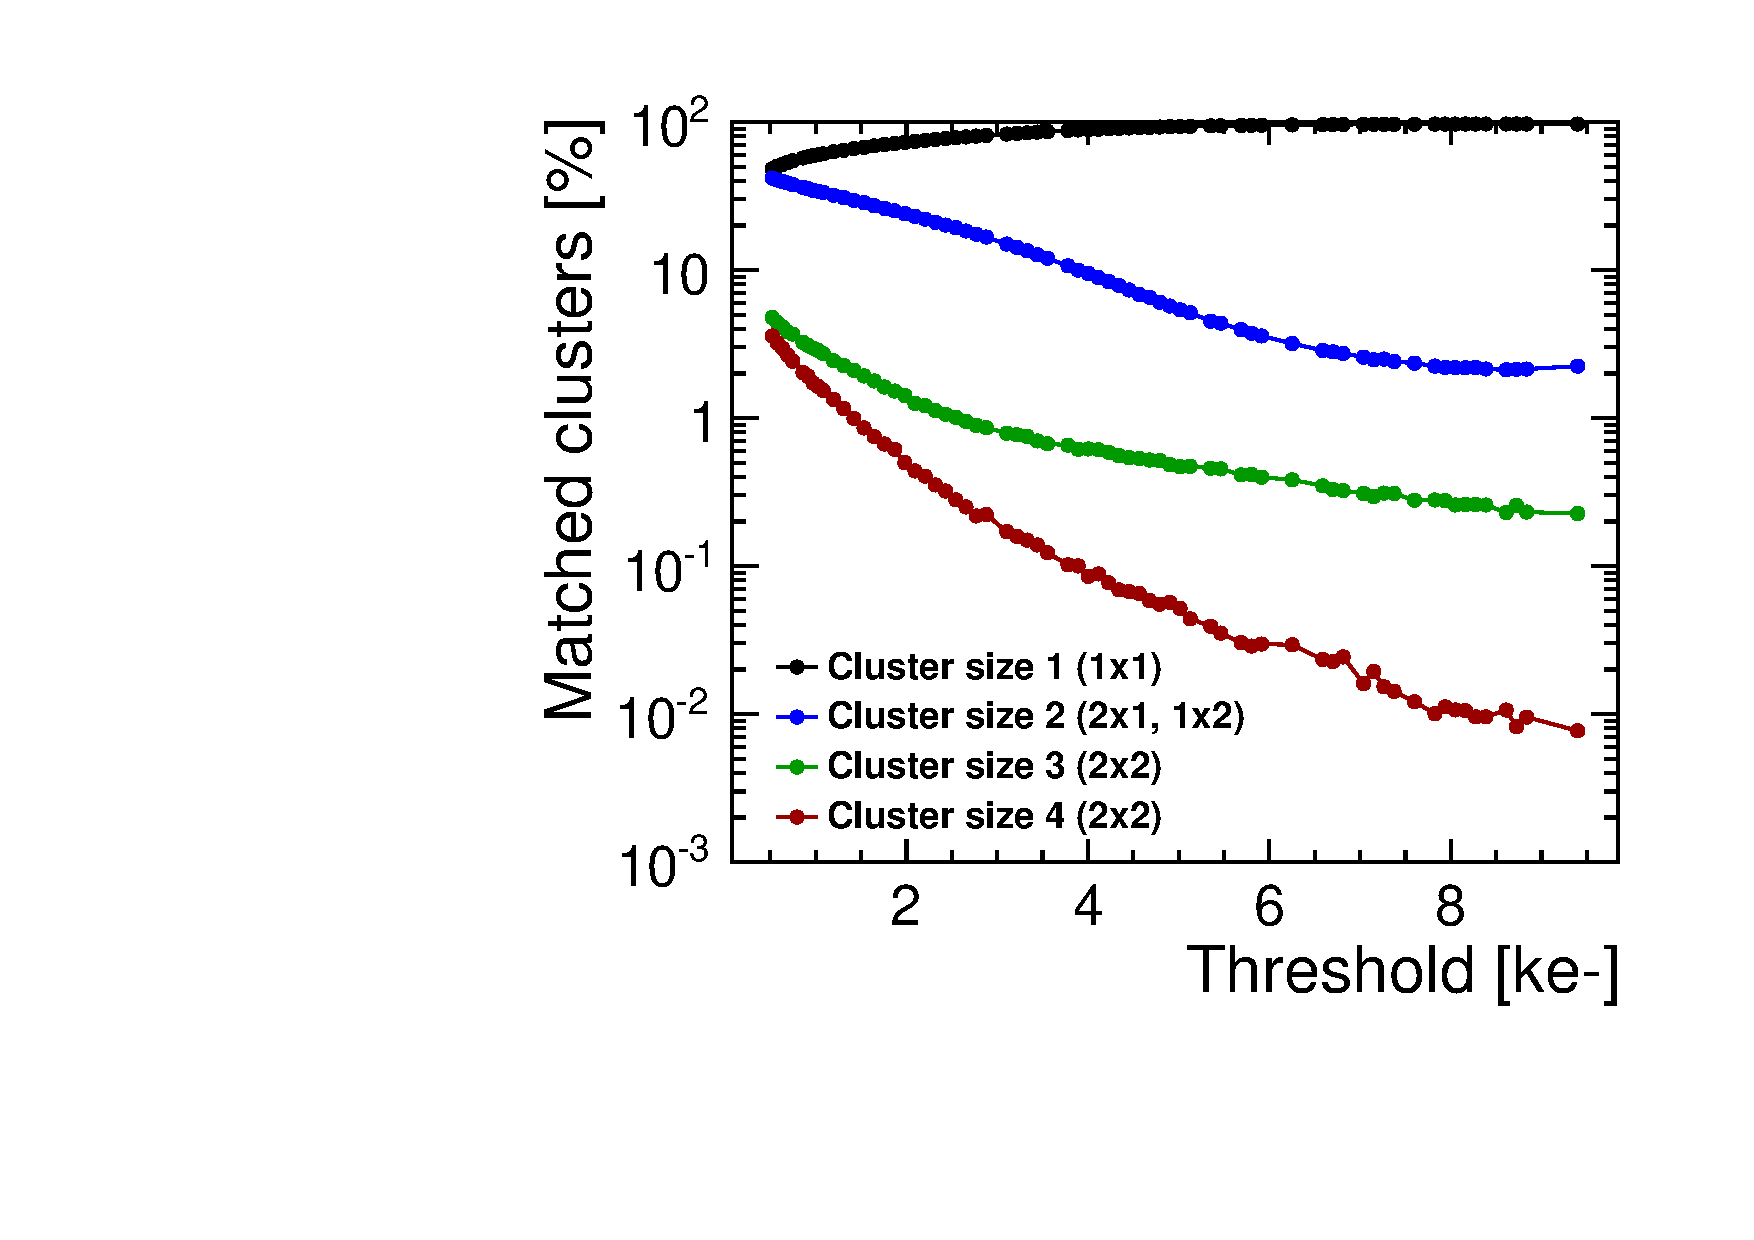
\includegraphics[width=\textwidth]{./figures/TestBeam/cluSize_THLscan_W0005_F01.pdf}
    \caption{W5\_F1}
  \end{subfigure}
  \caption{Cluster sizes distribution as a function of the operating
    threshold for assemblies listed in \cref{tab:Timepix3Assemblies}.}
  \label{fig:clusterSize_vs_THLscan}
\end{figure}


%% --------------------------------------------- %%
\newpage
\section{Charge sharing as a function of the track position}

\cref{fig:chargeSharingTrack_W19_G7,fig:chargeSharingTrack_W5_E2,fig:chargeSharingTrack_W5_F1}
illustrate the track position within the pixel for 1 to 4-pixel
cluster sizes for a $50-150\,\micron$ sensors.

\begin{figure}[htbp] \centering
  \begin{subfigure}[b]{0.23\textwidth}
    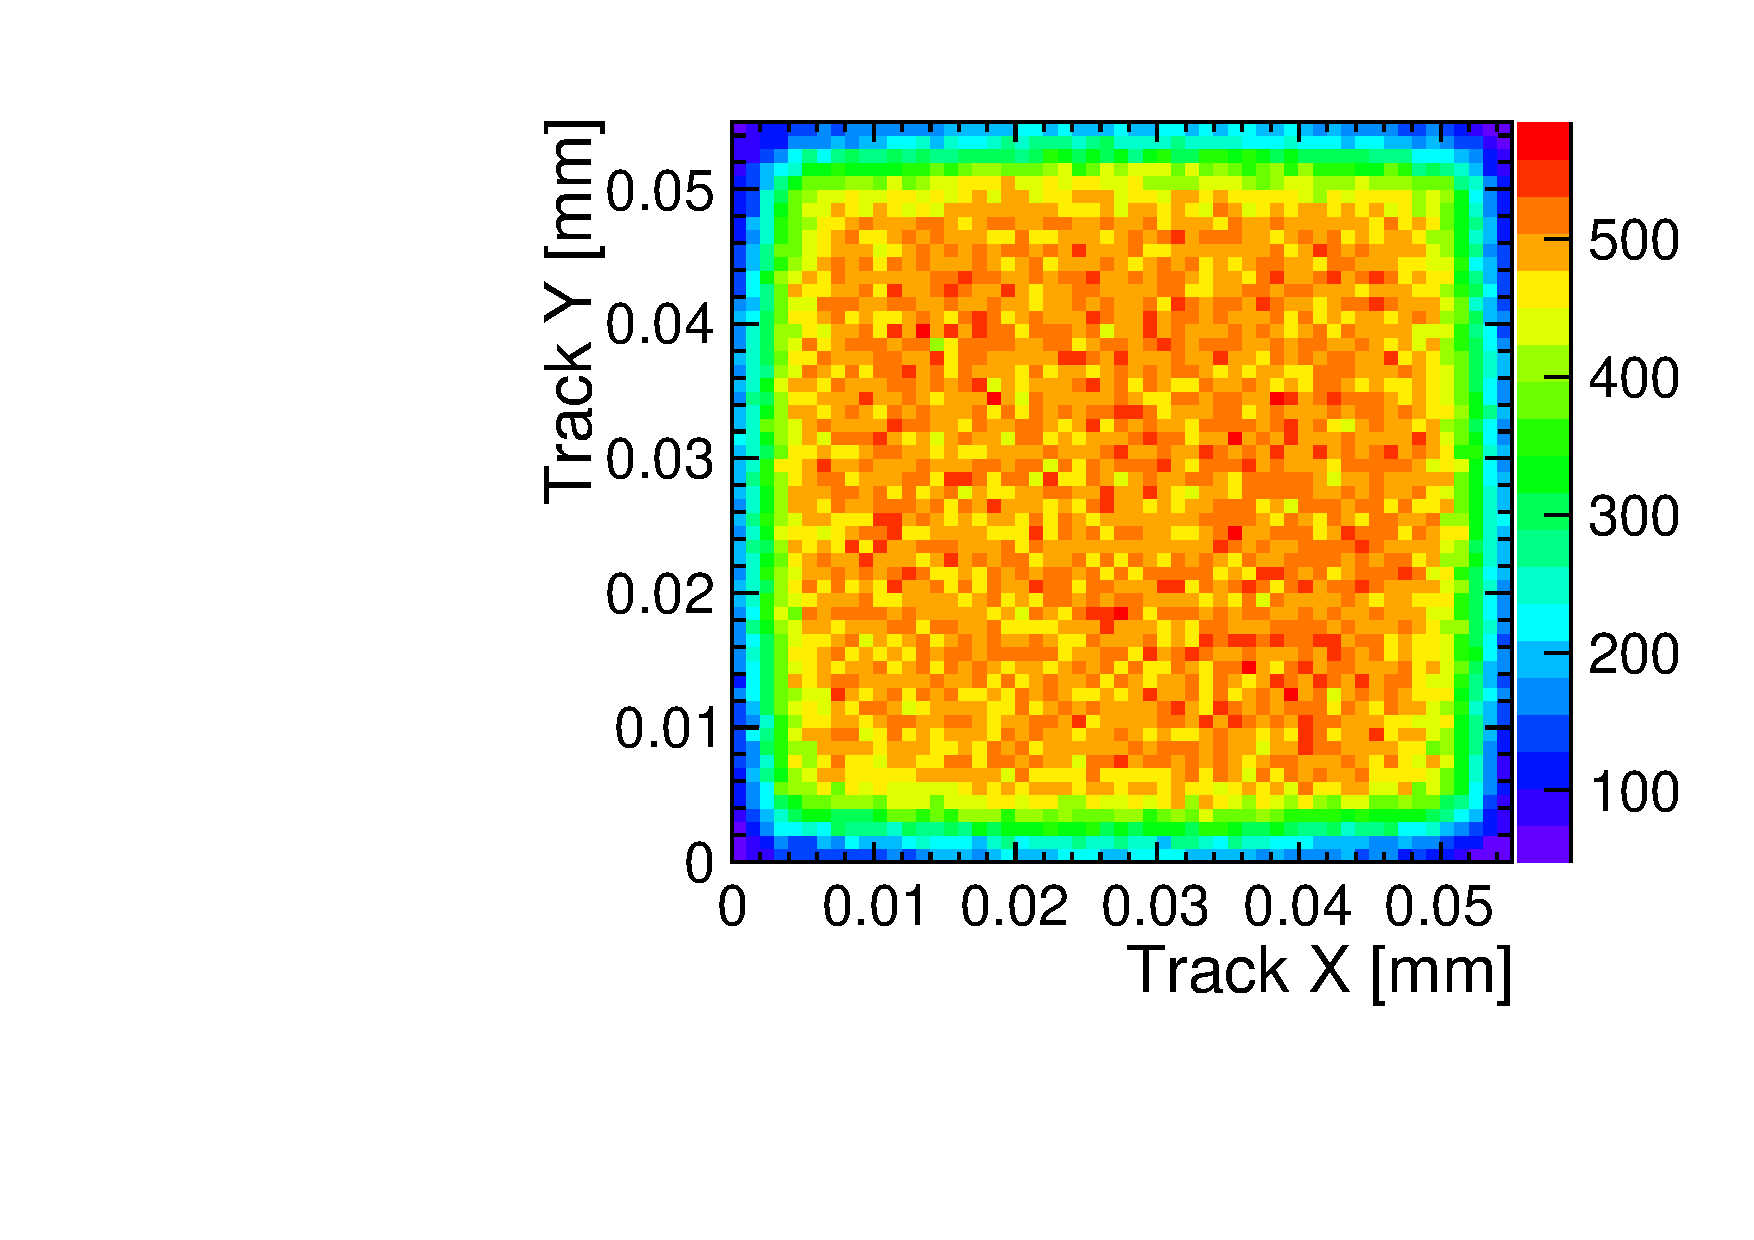
\includegraphics[width=\textwidth]{./figures/TestBeam/TrackPosWPixel_1hit_runW19_G7.pdf}
    \caption{Cluster size 1}
  \end{subfigure} \hfill
  \begin{subfigure}[b]{0.23\textwidth}
    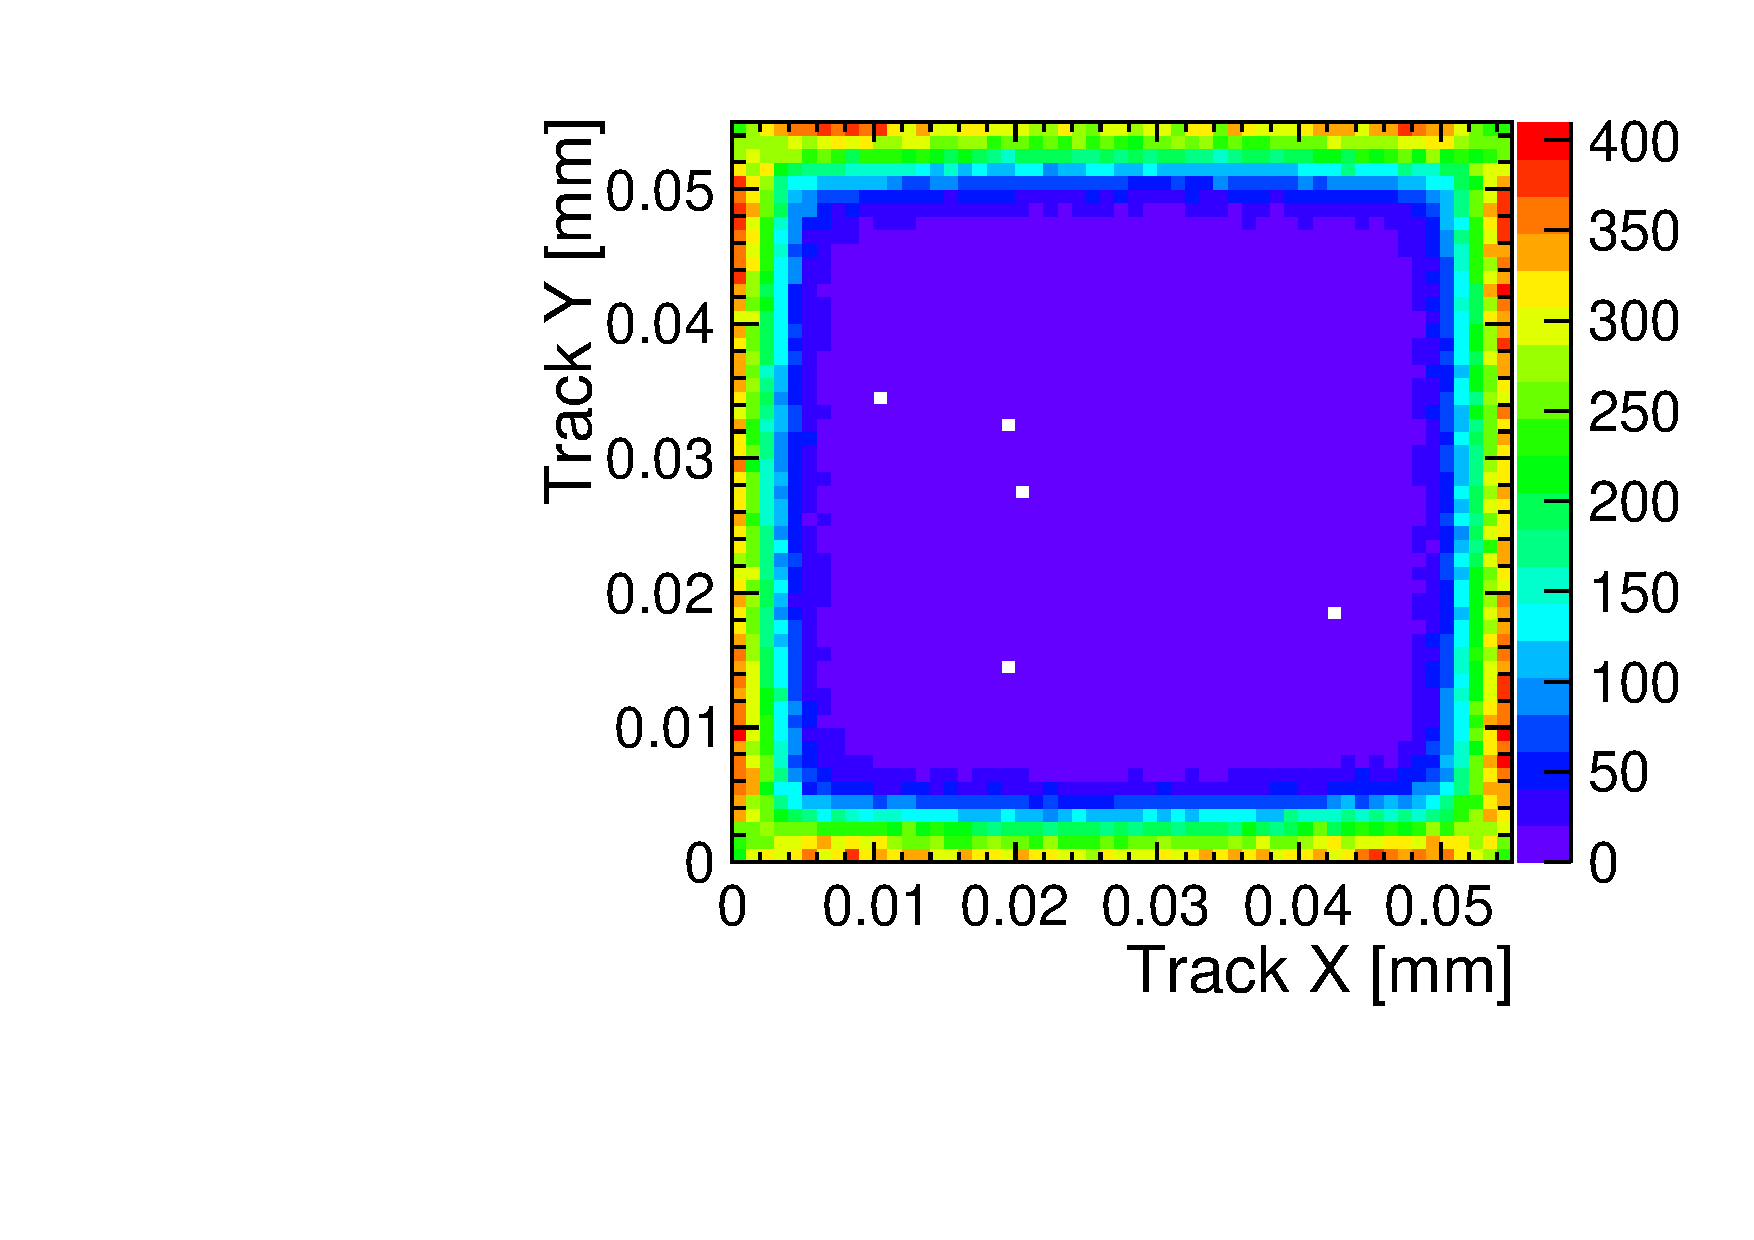
\includegraphics[width=\textwidth]{./figures/TestBeam/TrackPosWPixel_2hit_runW19_G7.pdf}
    \caption{Cluster size 2}
  \end{subfigure} \hfill
  \begin{subfigure}[b]{0.23\textwidth}
    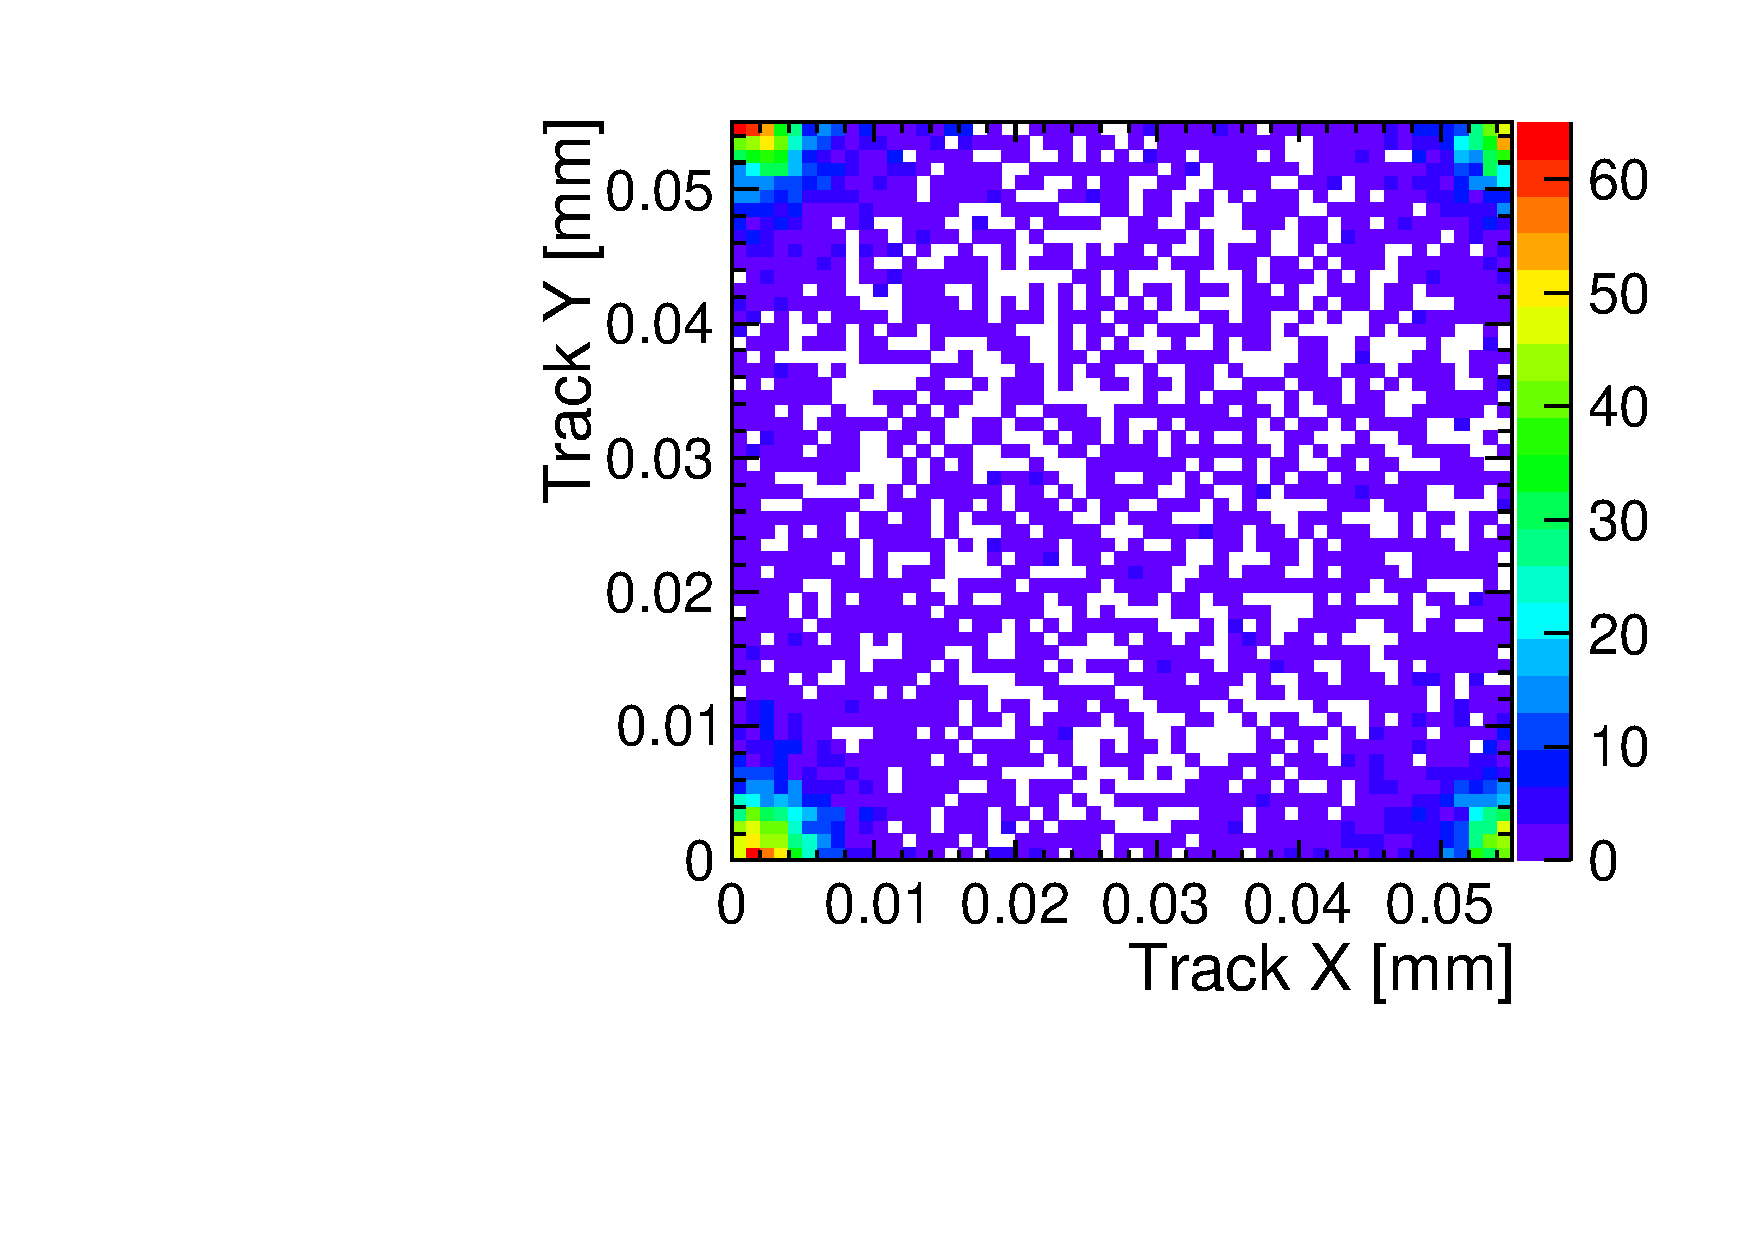
\includegraphics[width=\textwidth]{./figures/TestBeam/TrackPosWPixel_3hit_runW19_G7.pdf}
    \caption{Cluster size 3}
  \end{subfigure} \hfill
  \begin{subfigure}[b]{0.23\textwidth}
    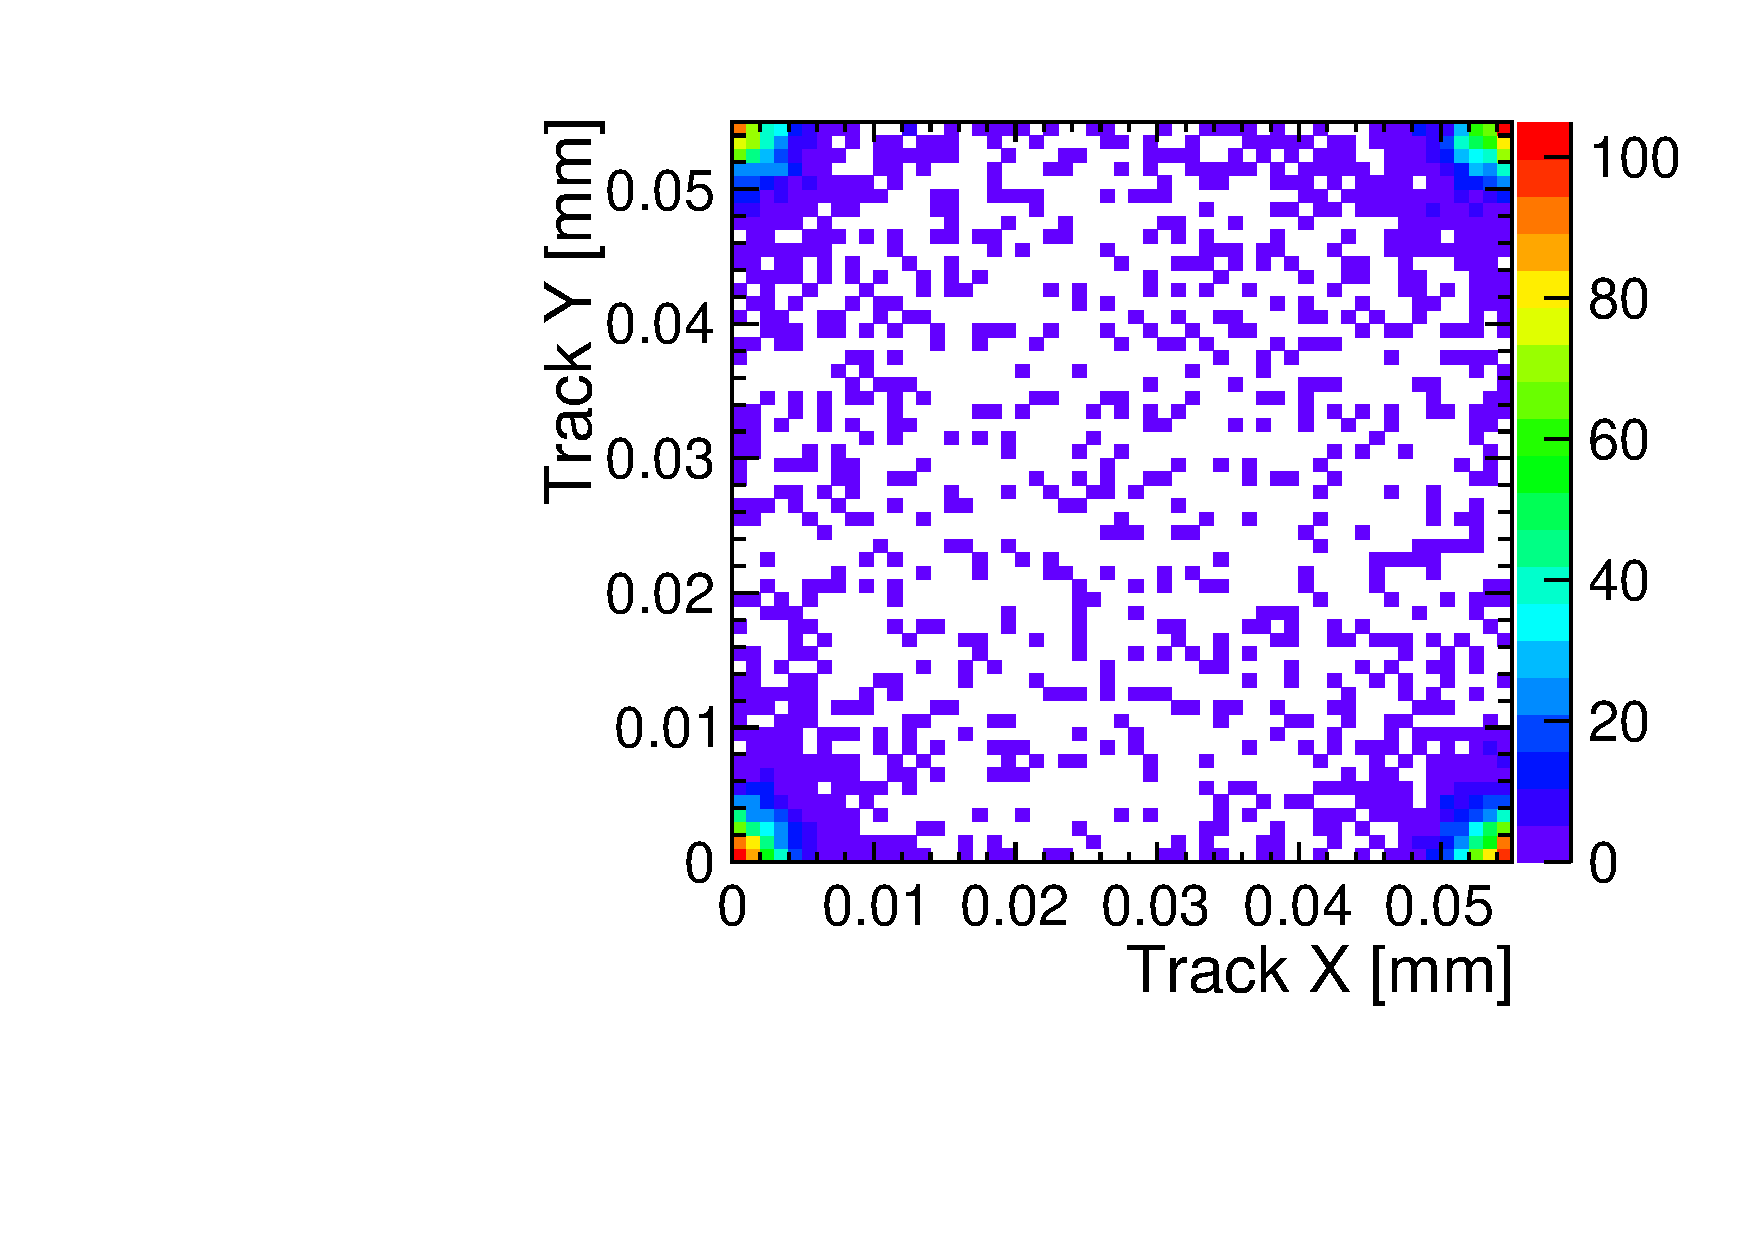
\includegraphics[width=\textwidth]{./figures/TestBeam/TrackPosWPixel_4hit_runW19_G7.pdf}
    \caption{Cluster size 4}
  \end{subfigure}
  \caption{Extrapolated track position within the pixel for 1 to 4-hit
    cluster sizes for a $50\,\micron$ sensor (assembly W19\_G7). The
    assembly is operated at the nominal conditions.}
  \label{fig:chargeSharingTrack_W19_G7}
\end{figure}

\begin{figure}[htbp] \centering
  \begin{subfigure}[b]{0.23\textwidth}
    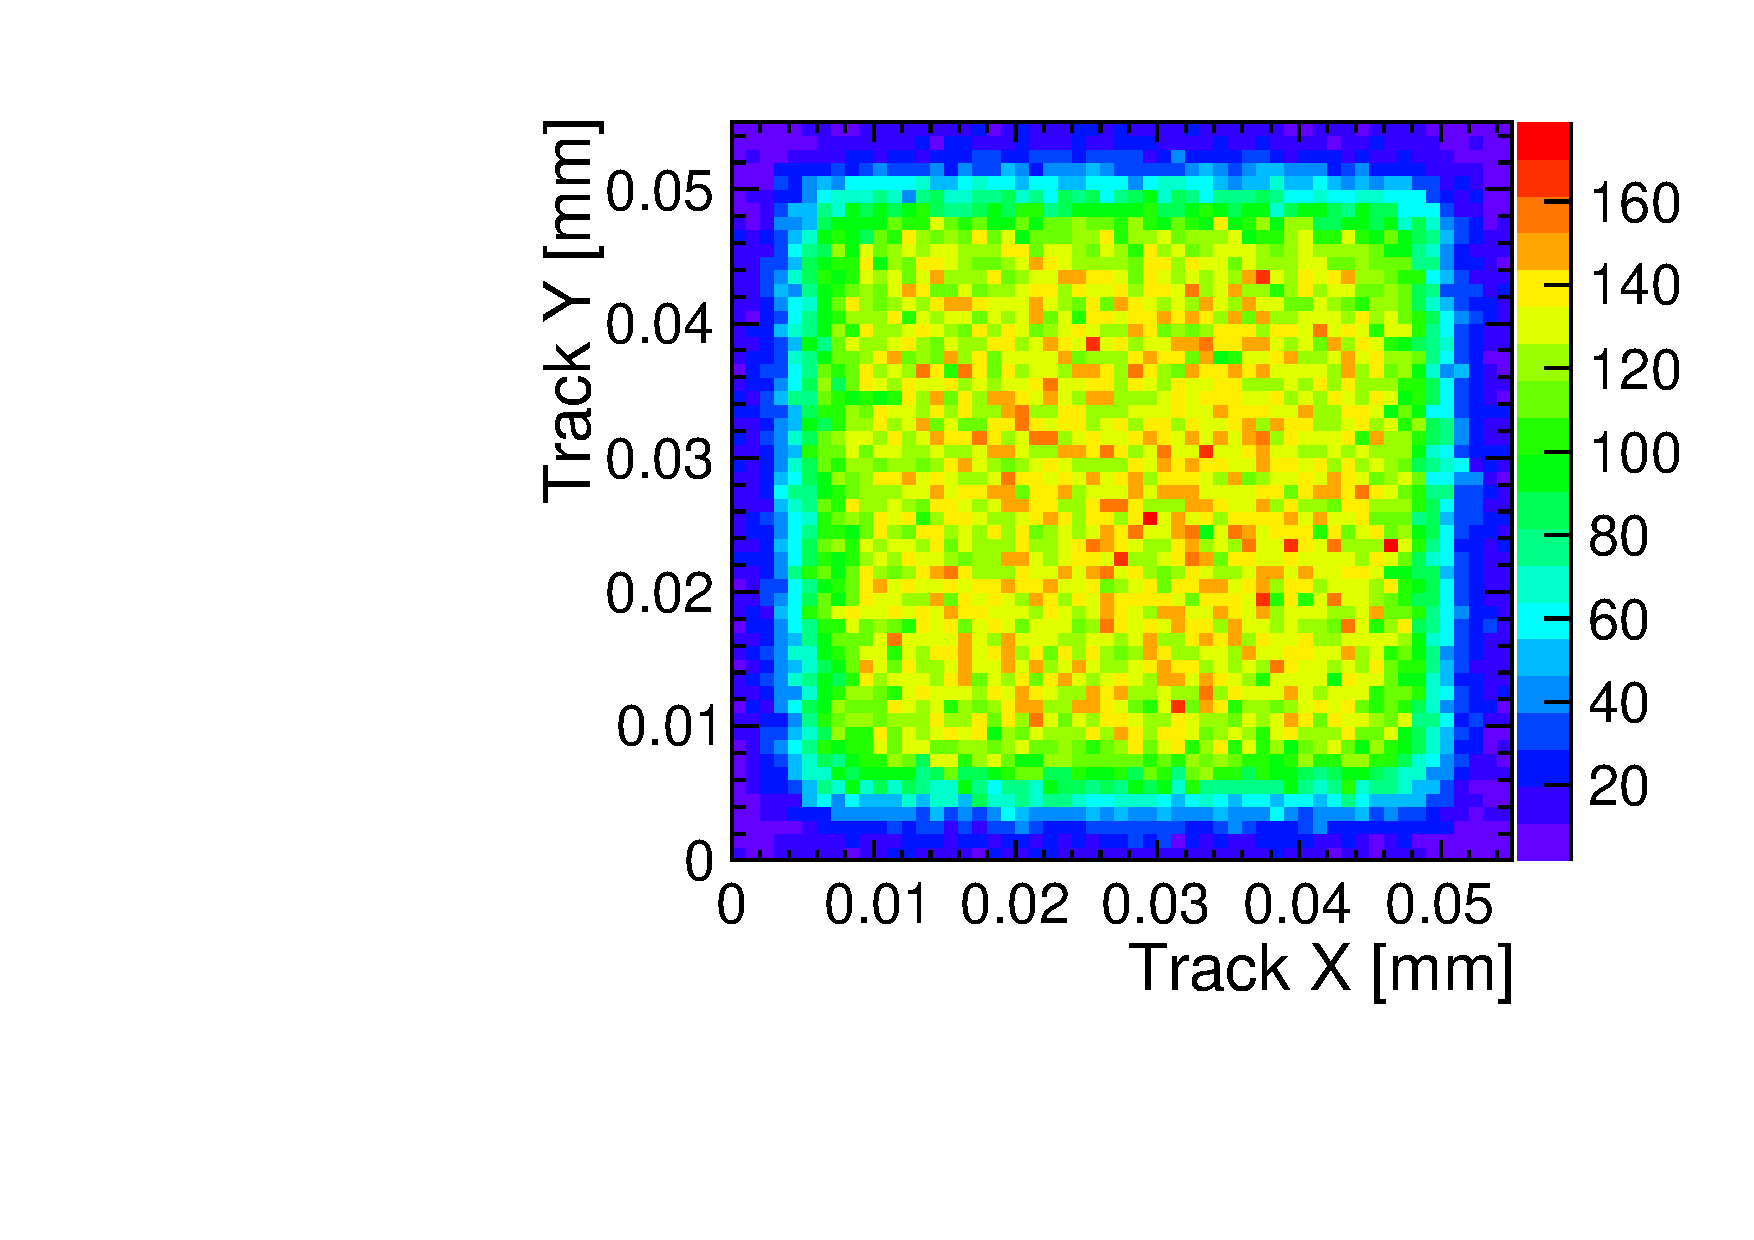
\includegraphics[width=\textwidth]{./figures/TestBeam/TrackPosWPixel_1hit_runW5_E2.pdf}
    \caption{Cluster size 1}
  \end{subfigure} \hfill
  \begin{subfigure}[b]{0.23\textwidth}
    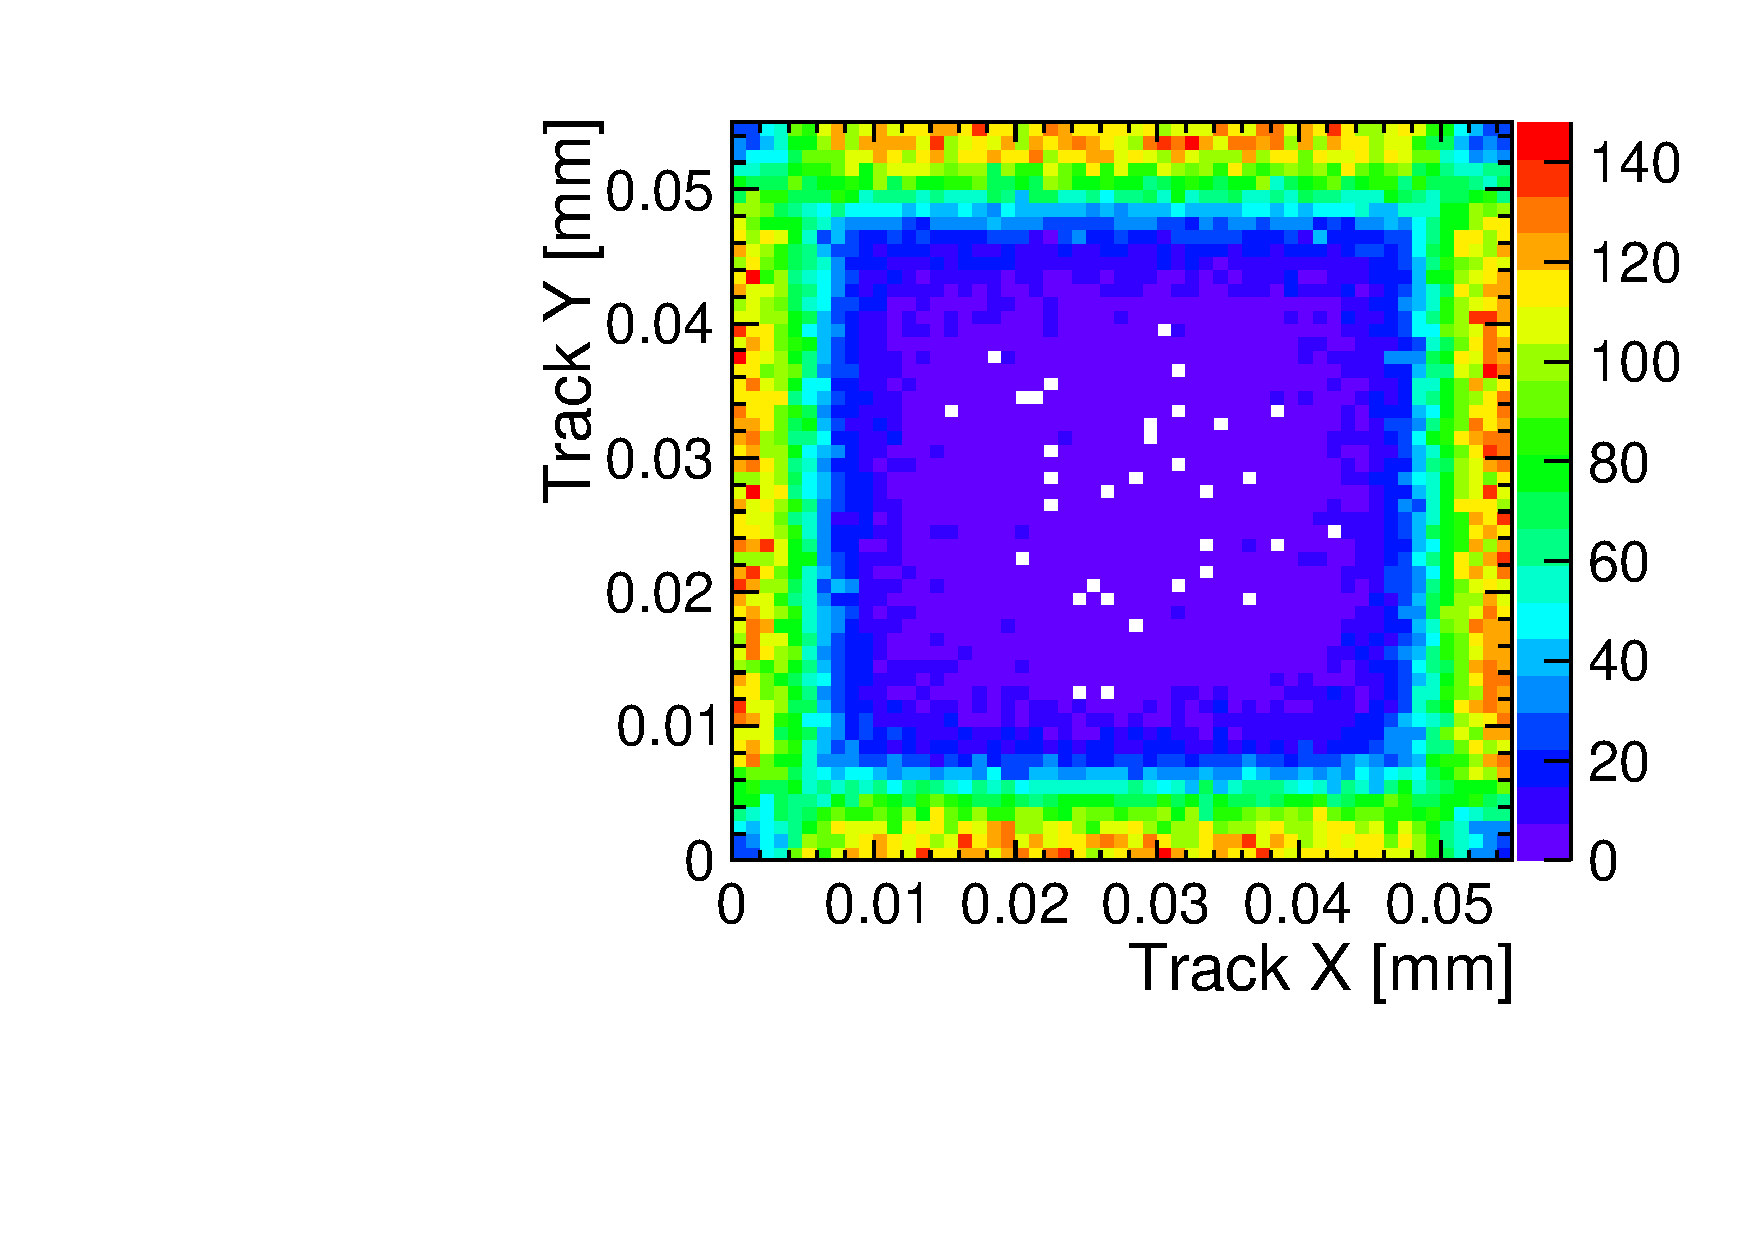
\includegraphics[width=\textwidth]{./figures/TestBeam/TrackPosWPixel_2hit_runW5_E2.pdf}
    \caption{Cluster size 2}
  \end{subfigure} \hfill
  \begin{subfigure}[b]{0.23\textwidth}
    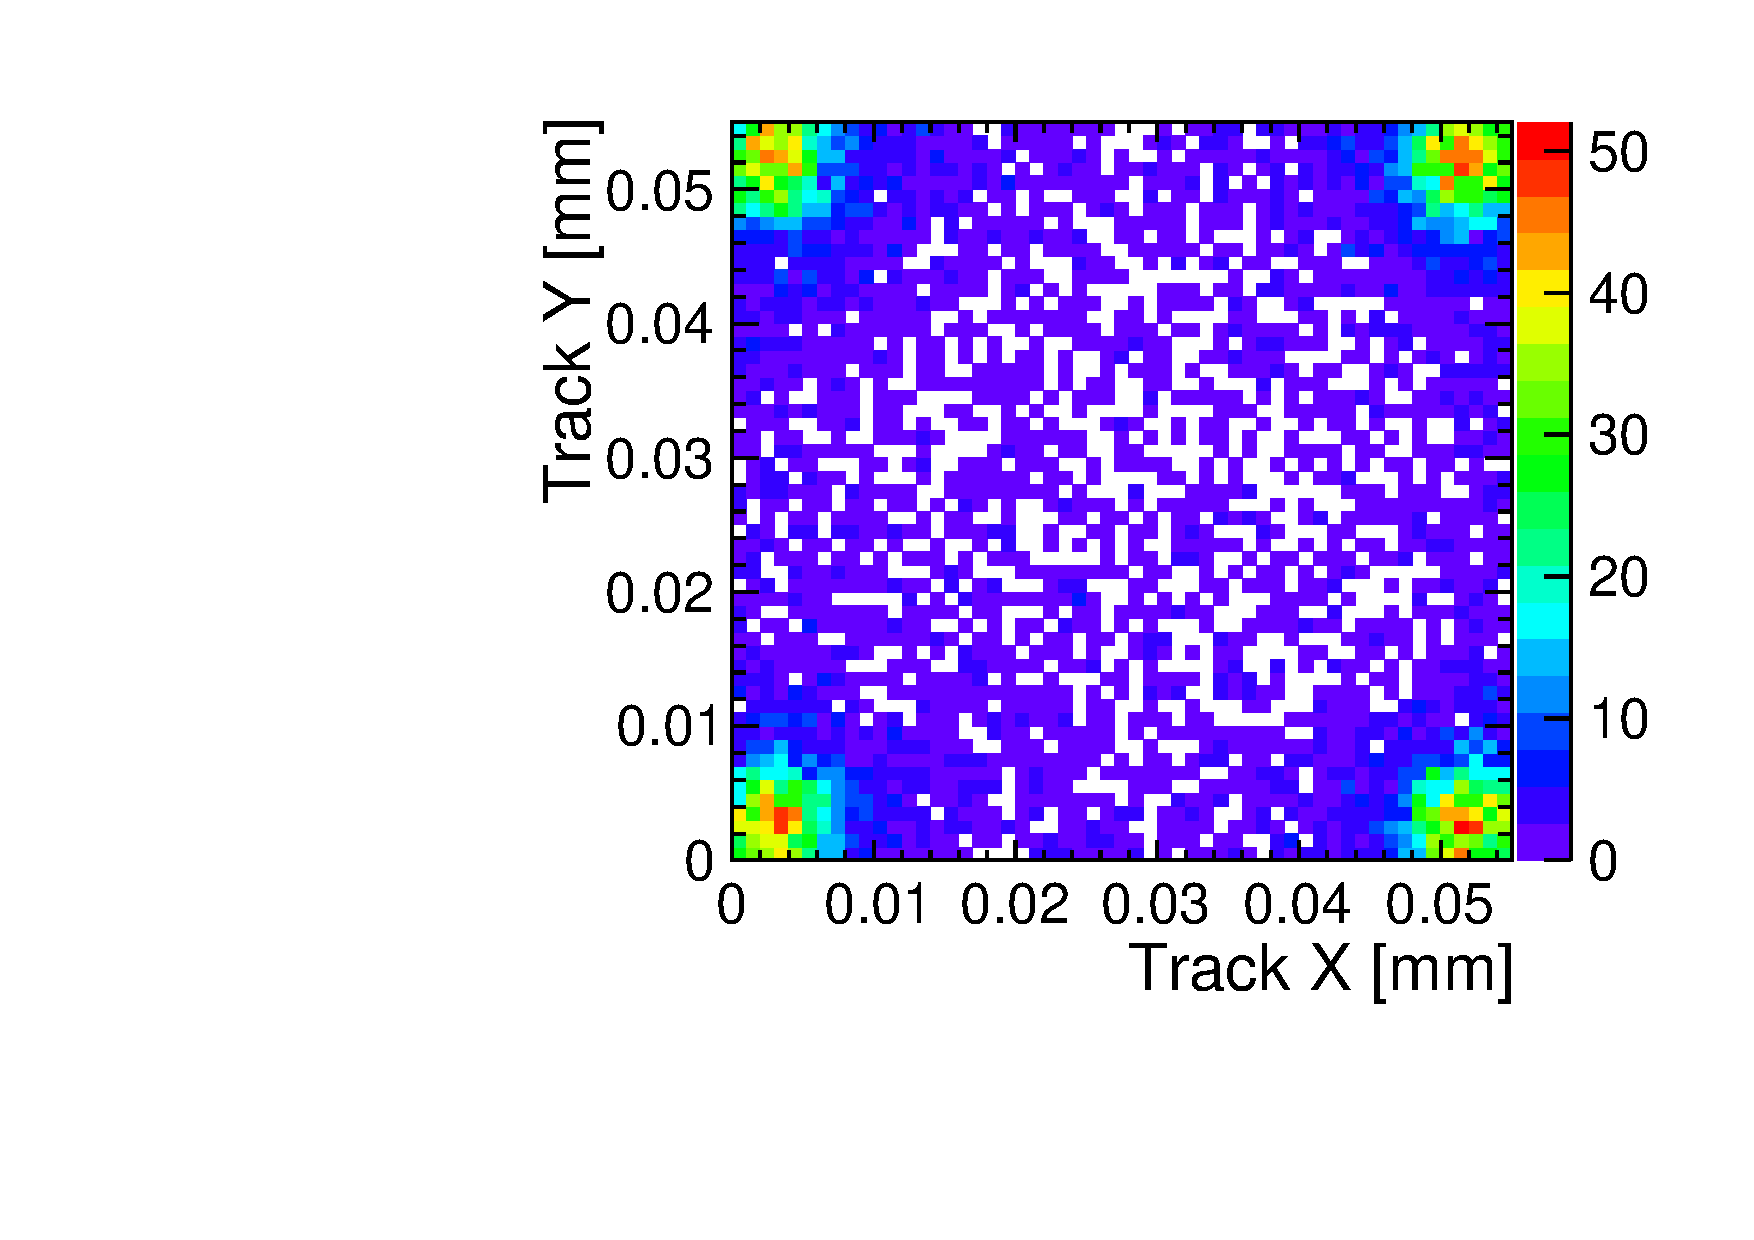
\includegraphics[width=\textwidth]{./figures/TestBeam/TrackPosWPixel_3hit_runW5_E2.pdf}
    \caption{Cluster size 3}
  \end{subfigure} \hfill
  \begin{subfigure}[b]{0.23\textwidth}
    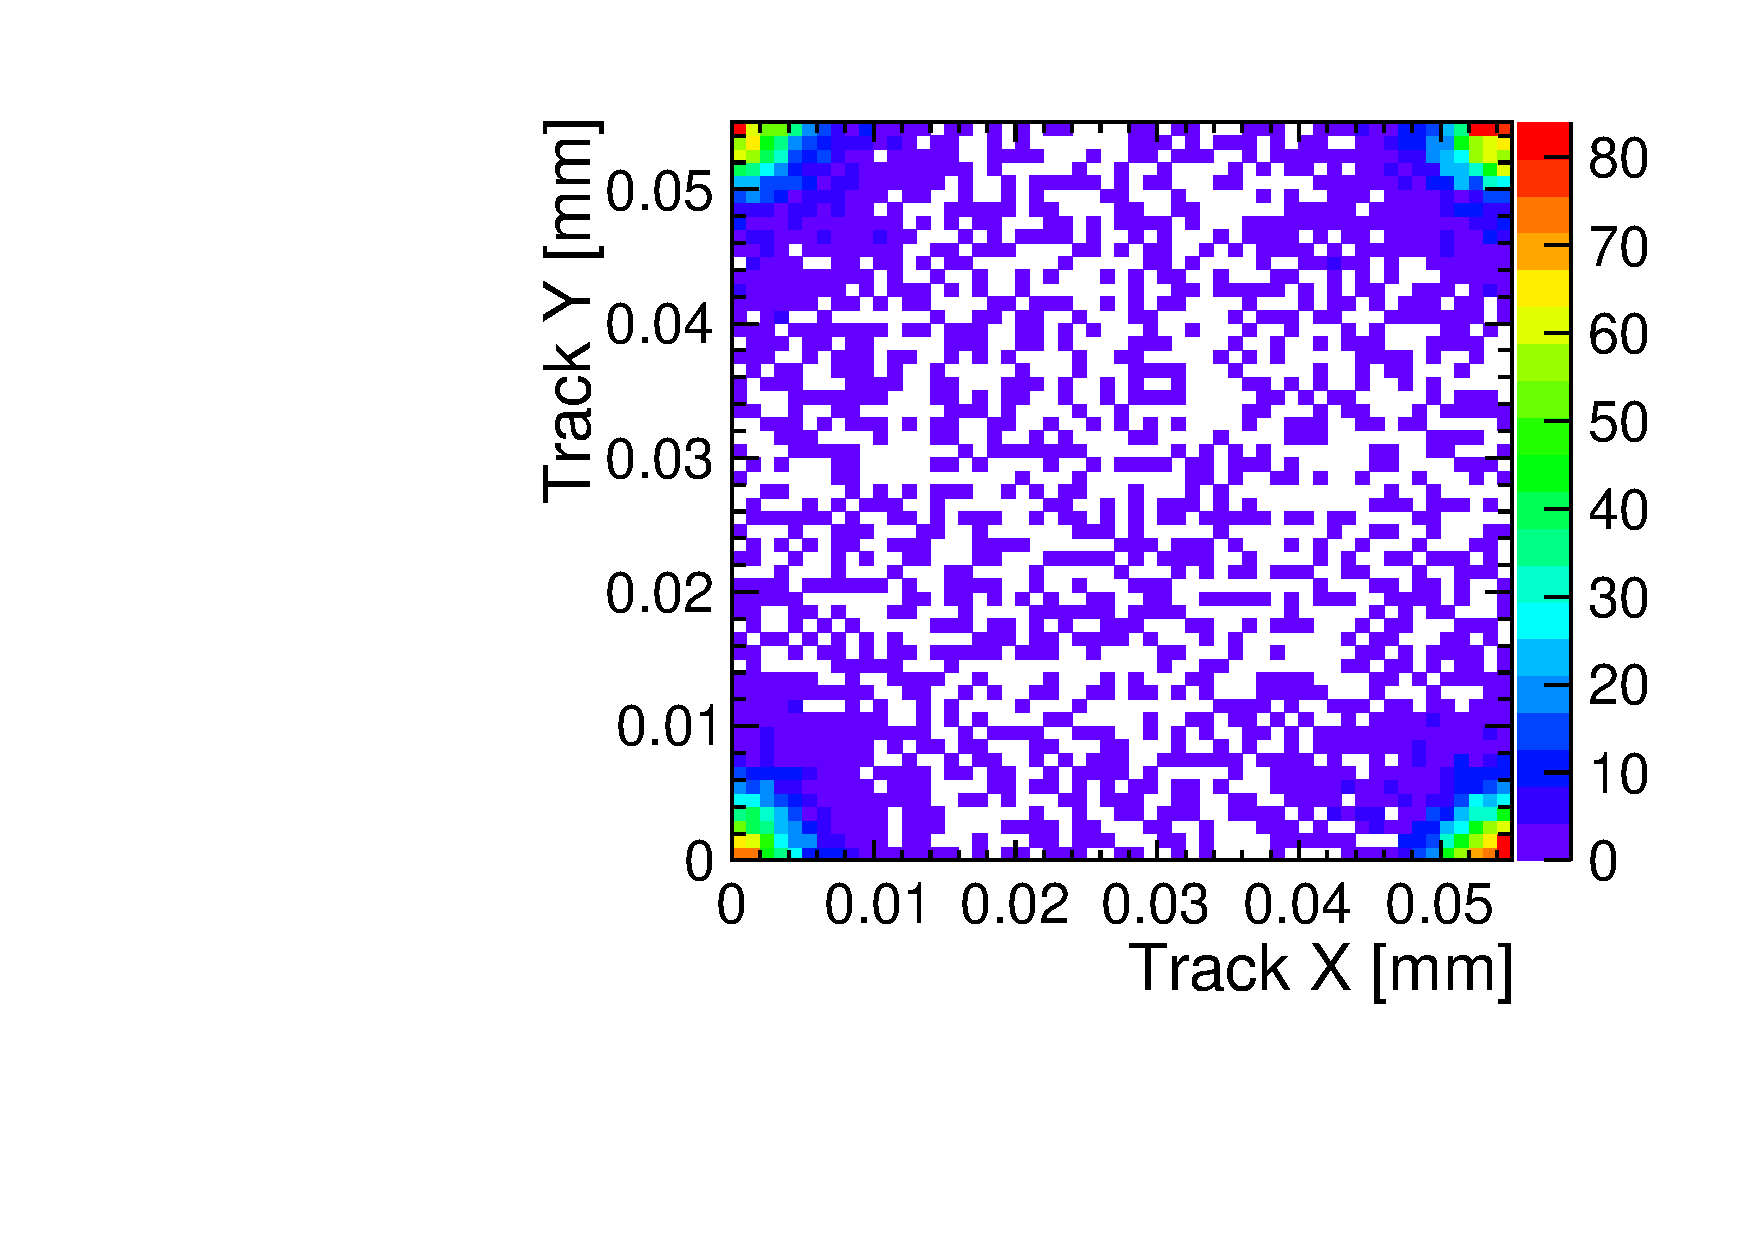
\includegraphics[width=\textwidth]{./figures/TestBeam/TrackPosWPixel_4hit_runW5_E2.pdf}
    \caption{Cluster size 4}
  \end{subfigure}
  \caption{Extrapolated track position within the pixel for 1 to 4-hit
    cluster sizes for a $100\,\micron$ sensor (assembly W5\_E2). The
    assembly is operated at the nominal conditions.}
  \label{fig:chargeSharingTrack_W5_E2}
\end{figure}

\begin{figure}[htbp] \centering
  \begin{subfigure}[b]{0.23\textwidth}
    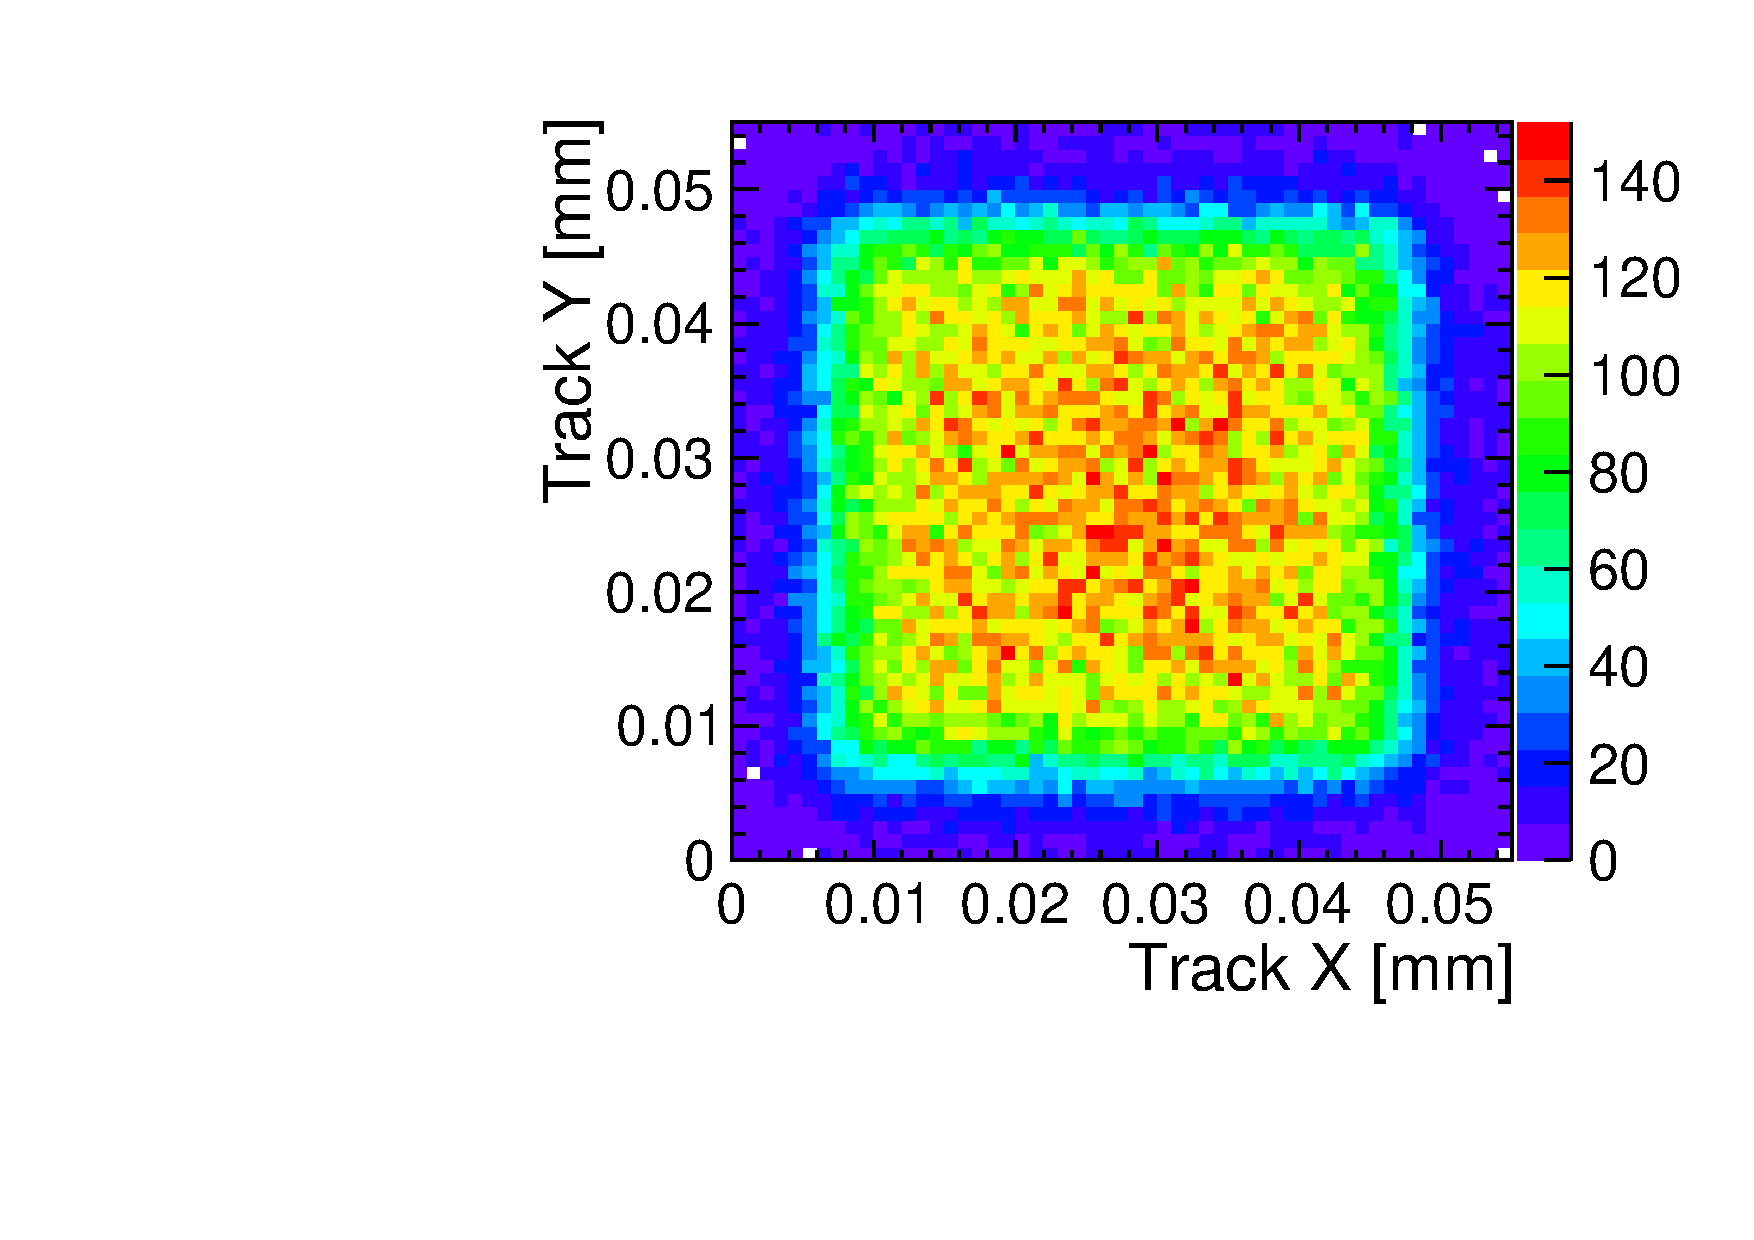
\includegraphics[width=\textwidth]{./figures/TestBeam/TrackPosWPixel_1hit_runW5_F1.pdf}
    \caption{Cluster size 1}
  \end{subfigure} \hfill
  \begin{subfigure}[b]{0.23\textwidth}
    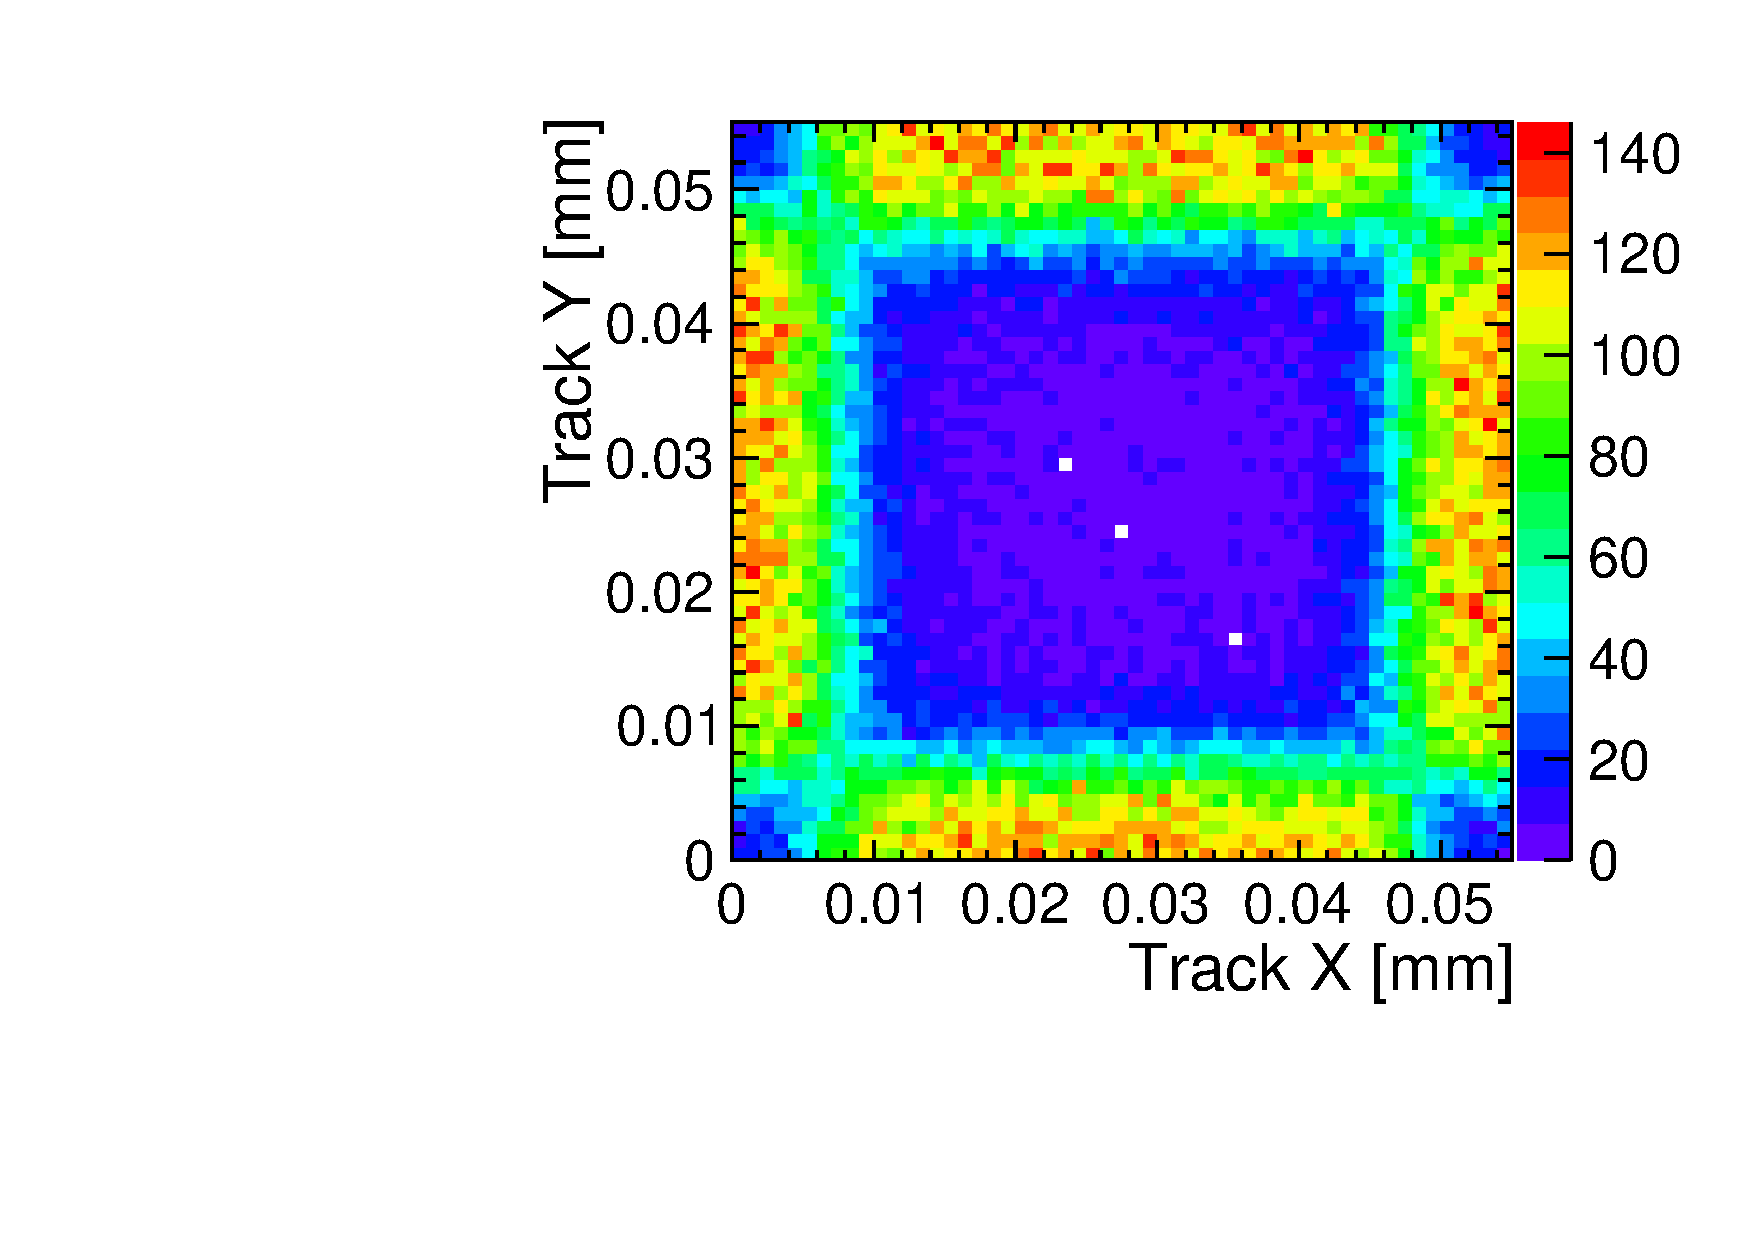
\includegraphics[width=\textwidth]{./figures/TestBeam/TrackPosWPixel_2hit_runW5_F1.pdf}
    \caption{Cluster size 2}
  \end{subfigure} \hfill
  \begin{subfigure}[b]{0.23\textwidth}
    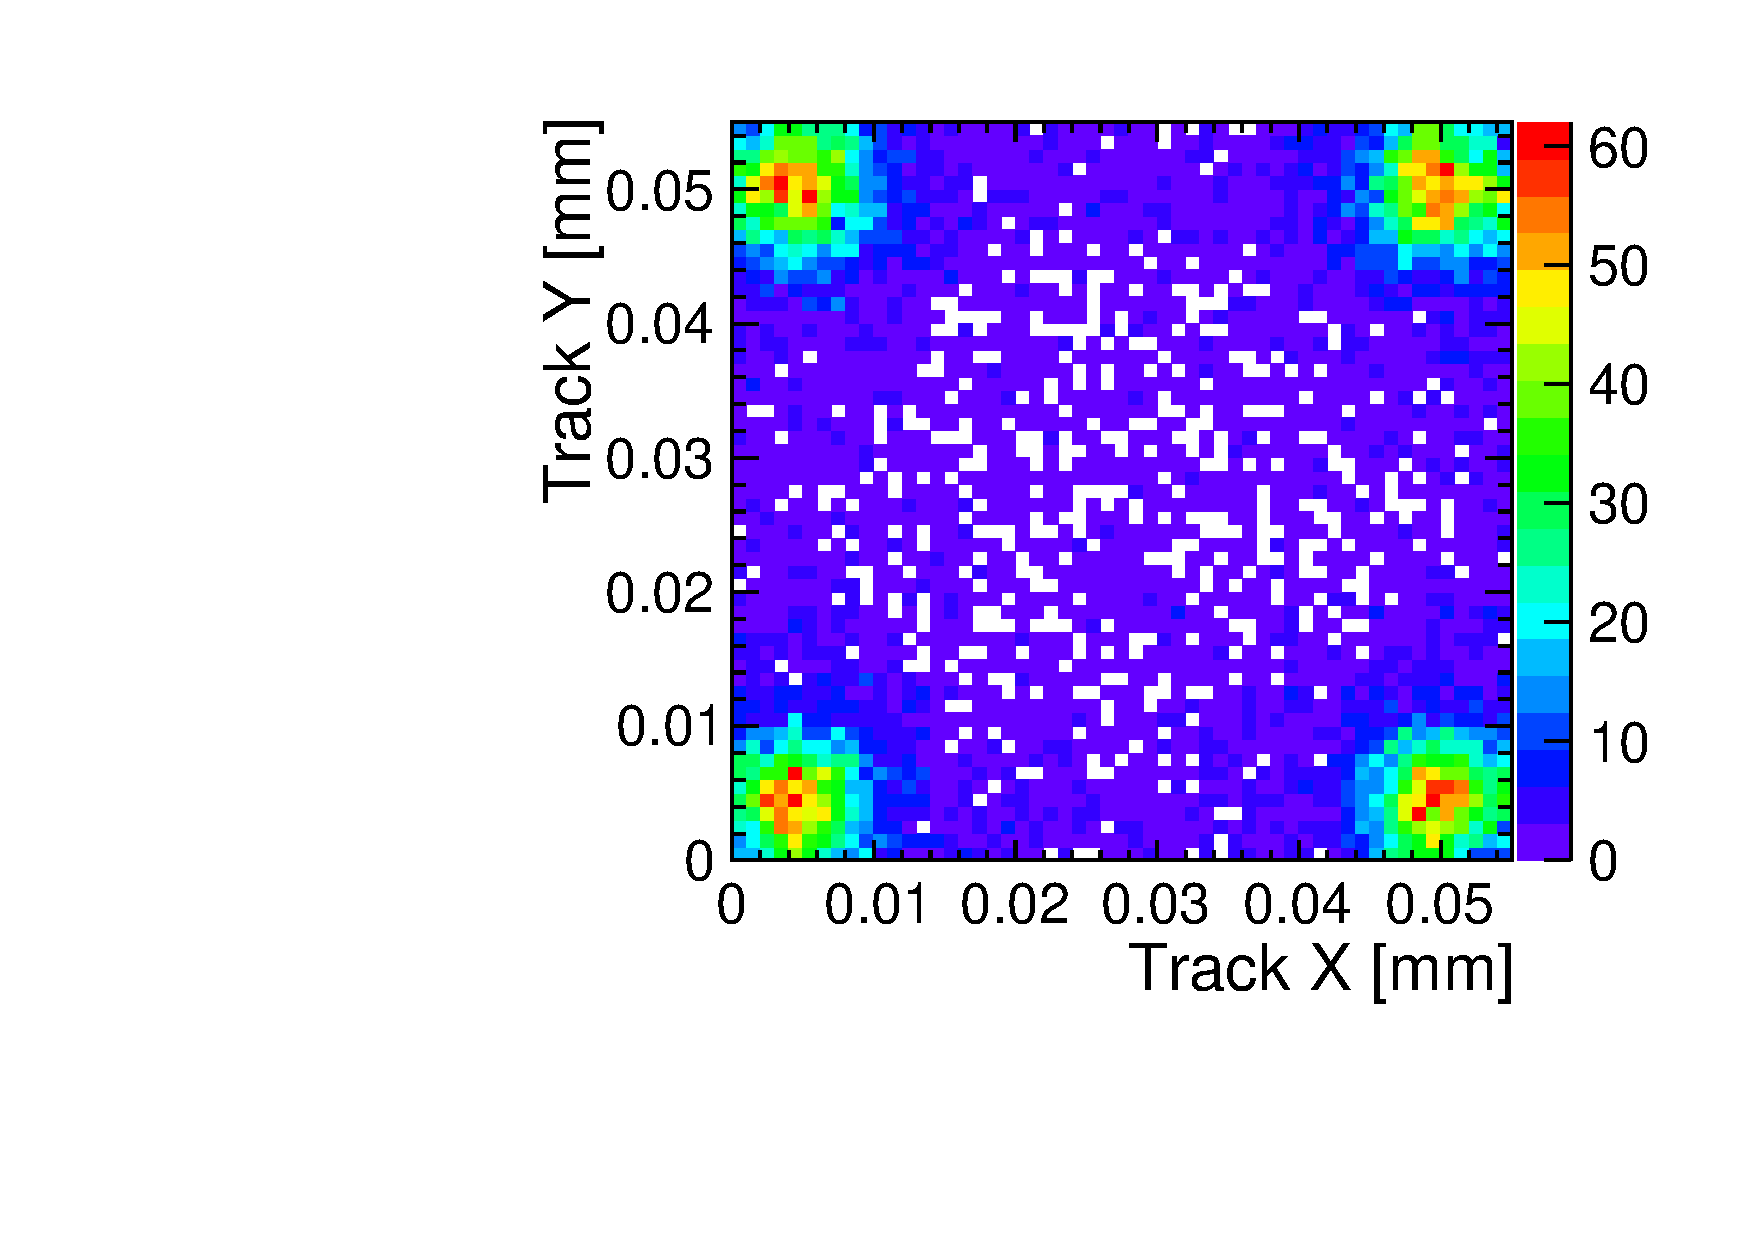
\includegraphics[width=\textwidth]{./figures/TestBeam/TrackPosWPixel_3hit_runW5_F1.pdf}
    \caption{Cluster size 3}
  \end{subfigure} \hfill
  \begin{subfigure}[b]{0.23\textwidth}
    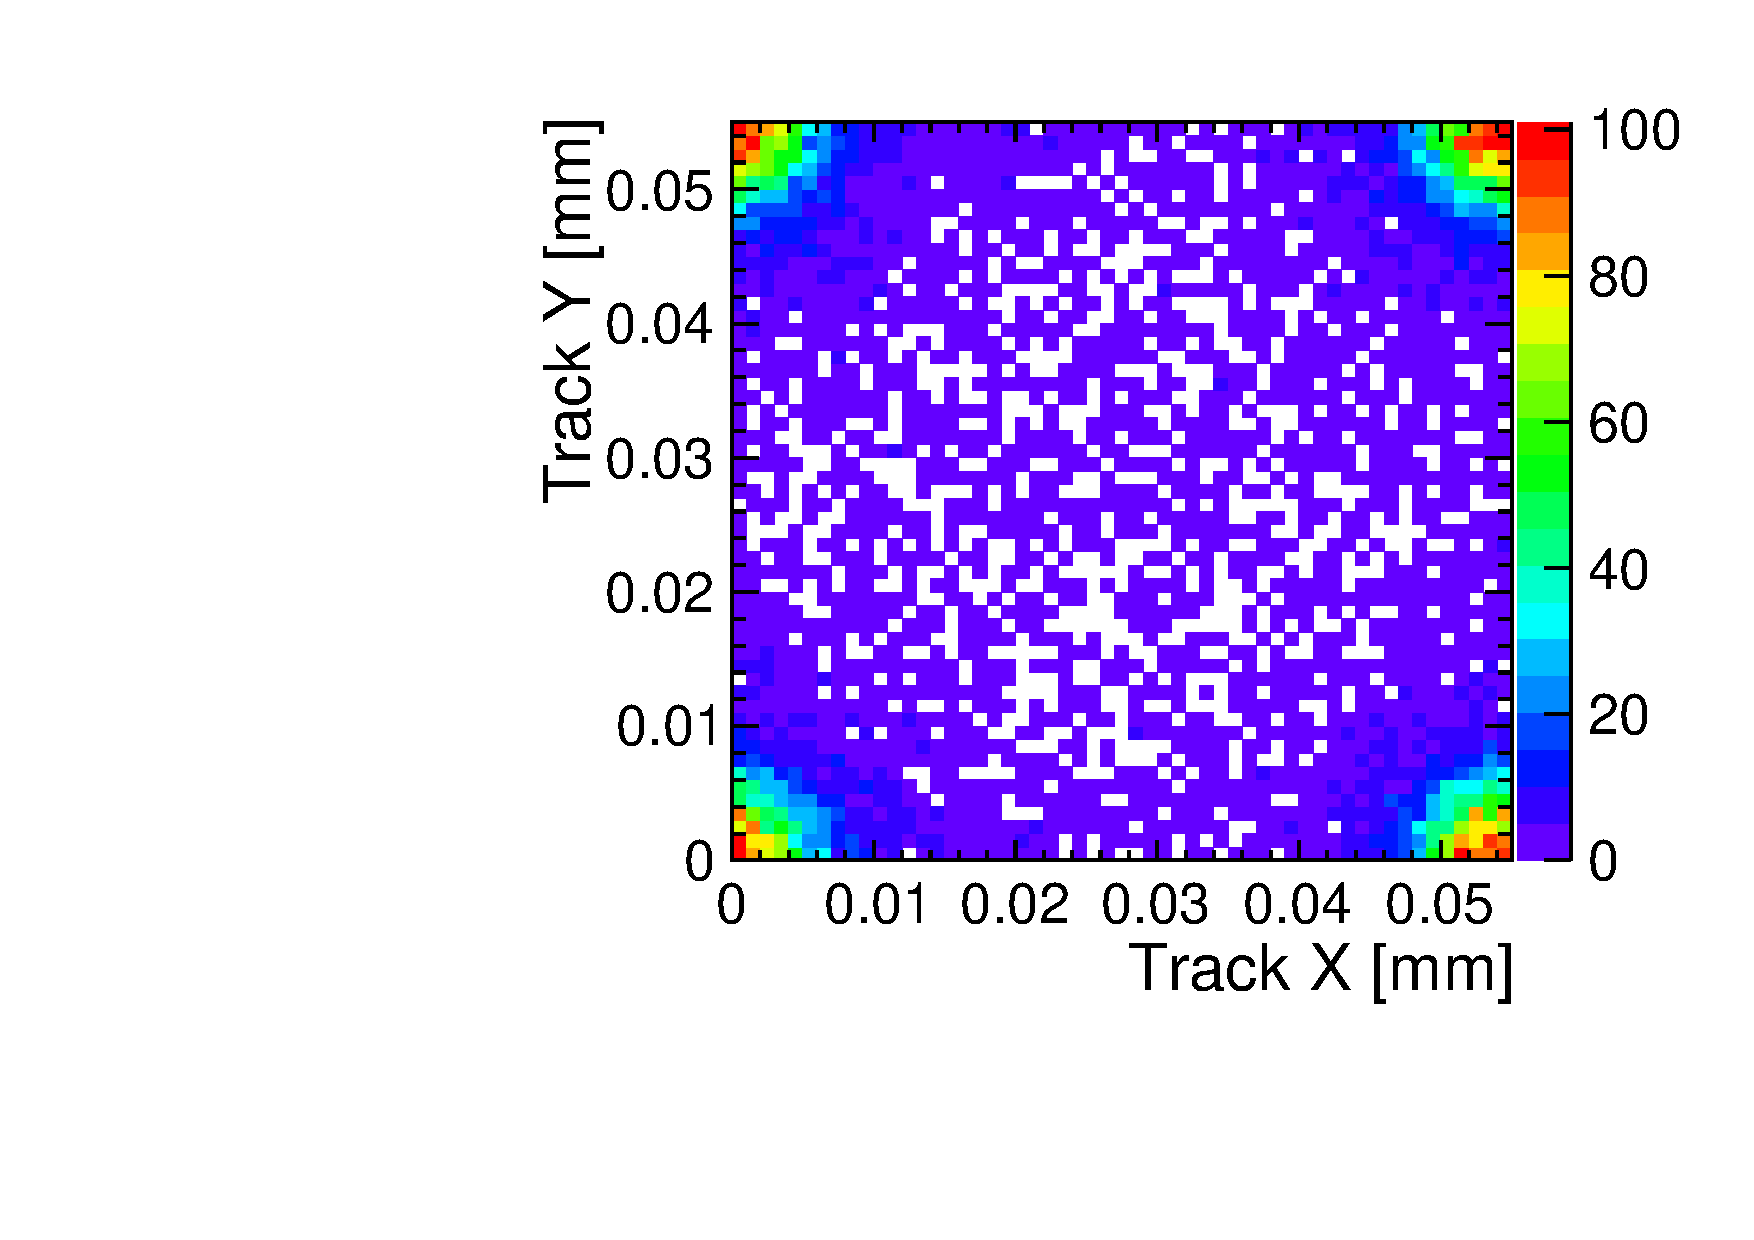
\includegraphics[width=\textwidth]{./figures/TestBeam/TrackPosWPixel_4hit_runW5_F1.pdf}
    \caption{Cluster size 4}
  \end{subfigure}
  \caption{Extrapolated track position within the pixel for 1 to 4-hit
    cluster sizes for a $150\,\micron$ sensor (assembly W5\_F1). The
    assembly is operated at the nominal conditions.}
  \label{fig:chargeSharingTrack_W5_F1}
\end{figure}

% \begin{figure}[htbp] \centering
%   \begin{subfigure}[b]{0.23\textwidth}
%     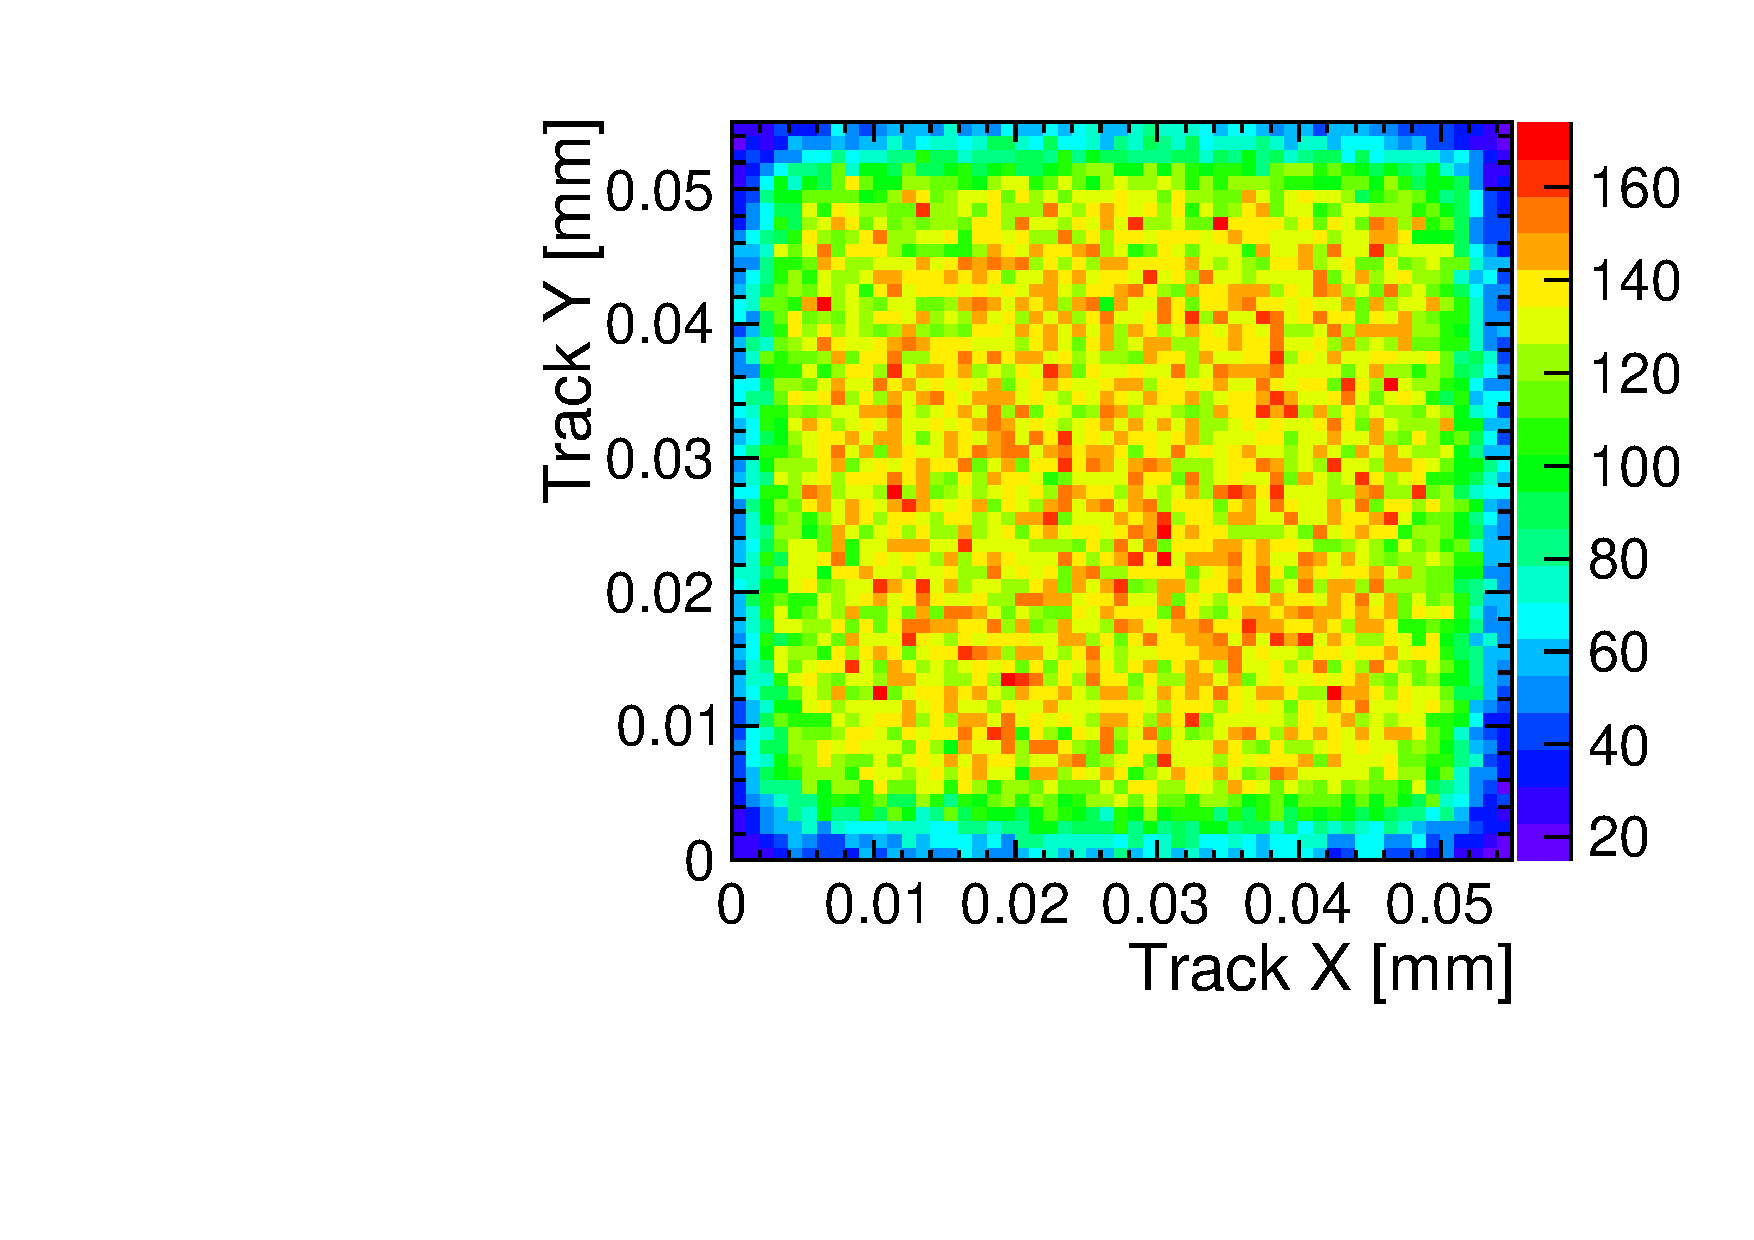
\includegraphics[width=\textwidth]{./figures/TestBeam/TrackPosWPixel_1hit_runW19_F7.pdf}
%     \caption{Cluster size 1}
%   \end{subfigure} \hfill
%   \begin{subfigure}[b]{0.23\textwidth}
%     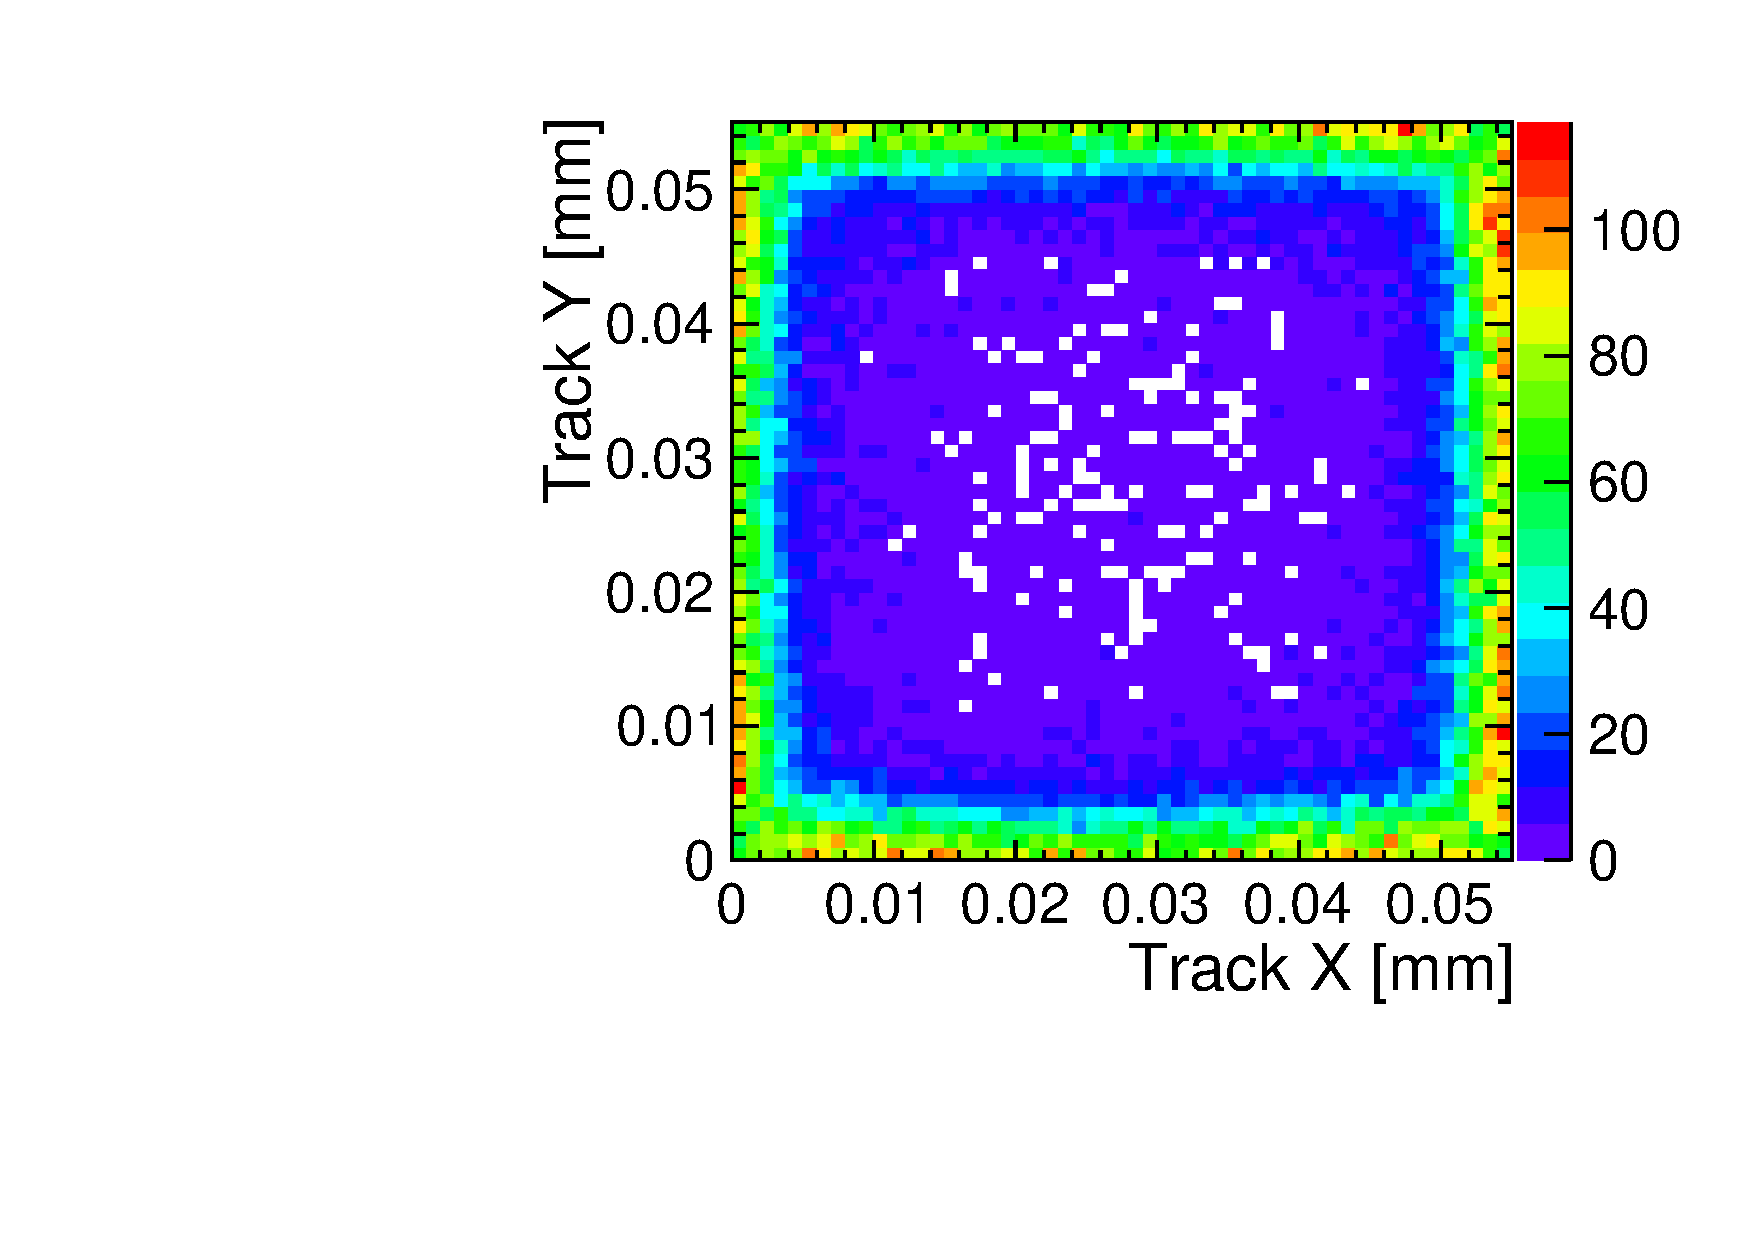
\includegraphics[width=\textwidth]{./figures/TestBeam/TrackPosWPixel_2hit_runW19_F7.pdf}
%     \caption{Cluster size 2}
%   \end{subfigure} \hfill
%   \begin{subfigure}[b]{0.23\textwidth}
%     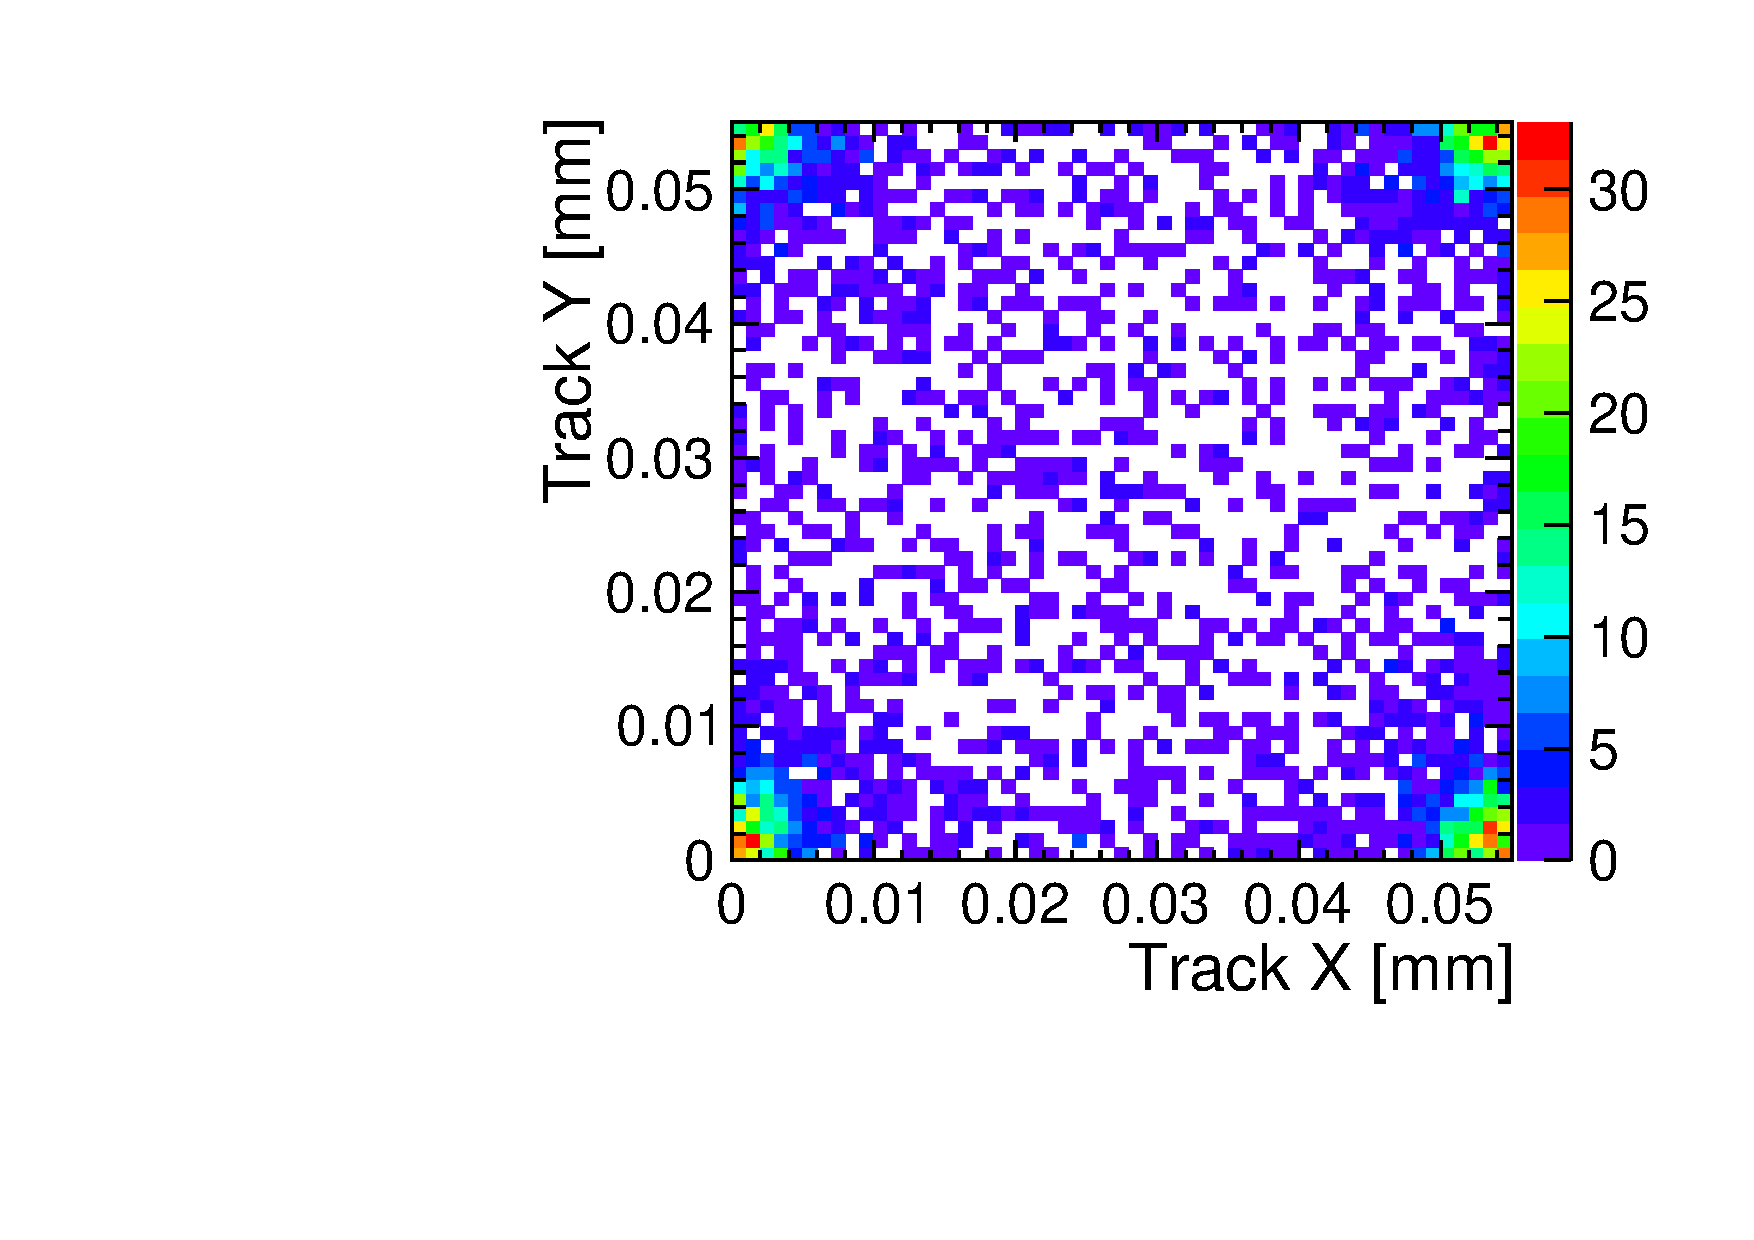
\includegraphics[width=\textwidth]{./figures/TestBeam/TrackPosWPixel_3hit_runW19_F7.pdf}
%     \caption{Cluster size 3}
%   \end{subfigure} \hfill
%   \begin{subfigure}[b]{0.23\textwidth}
%     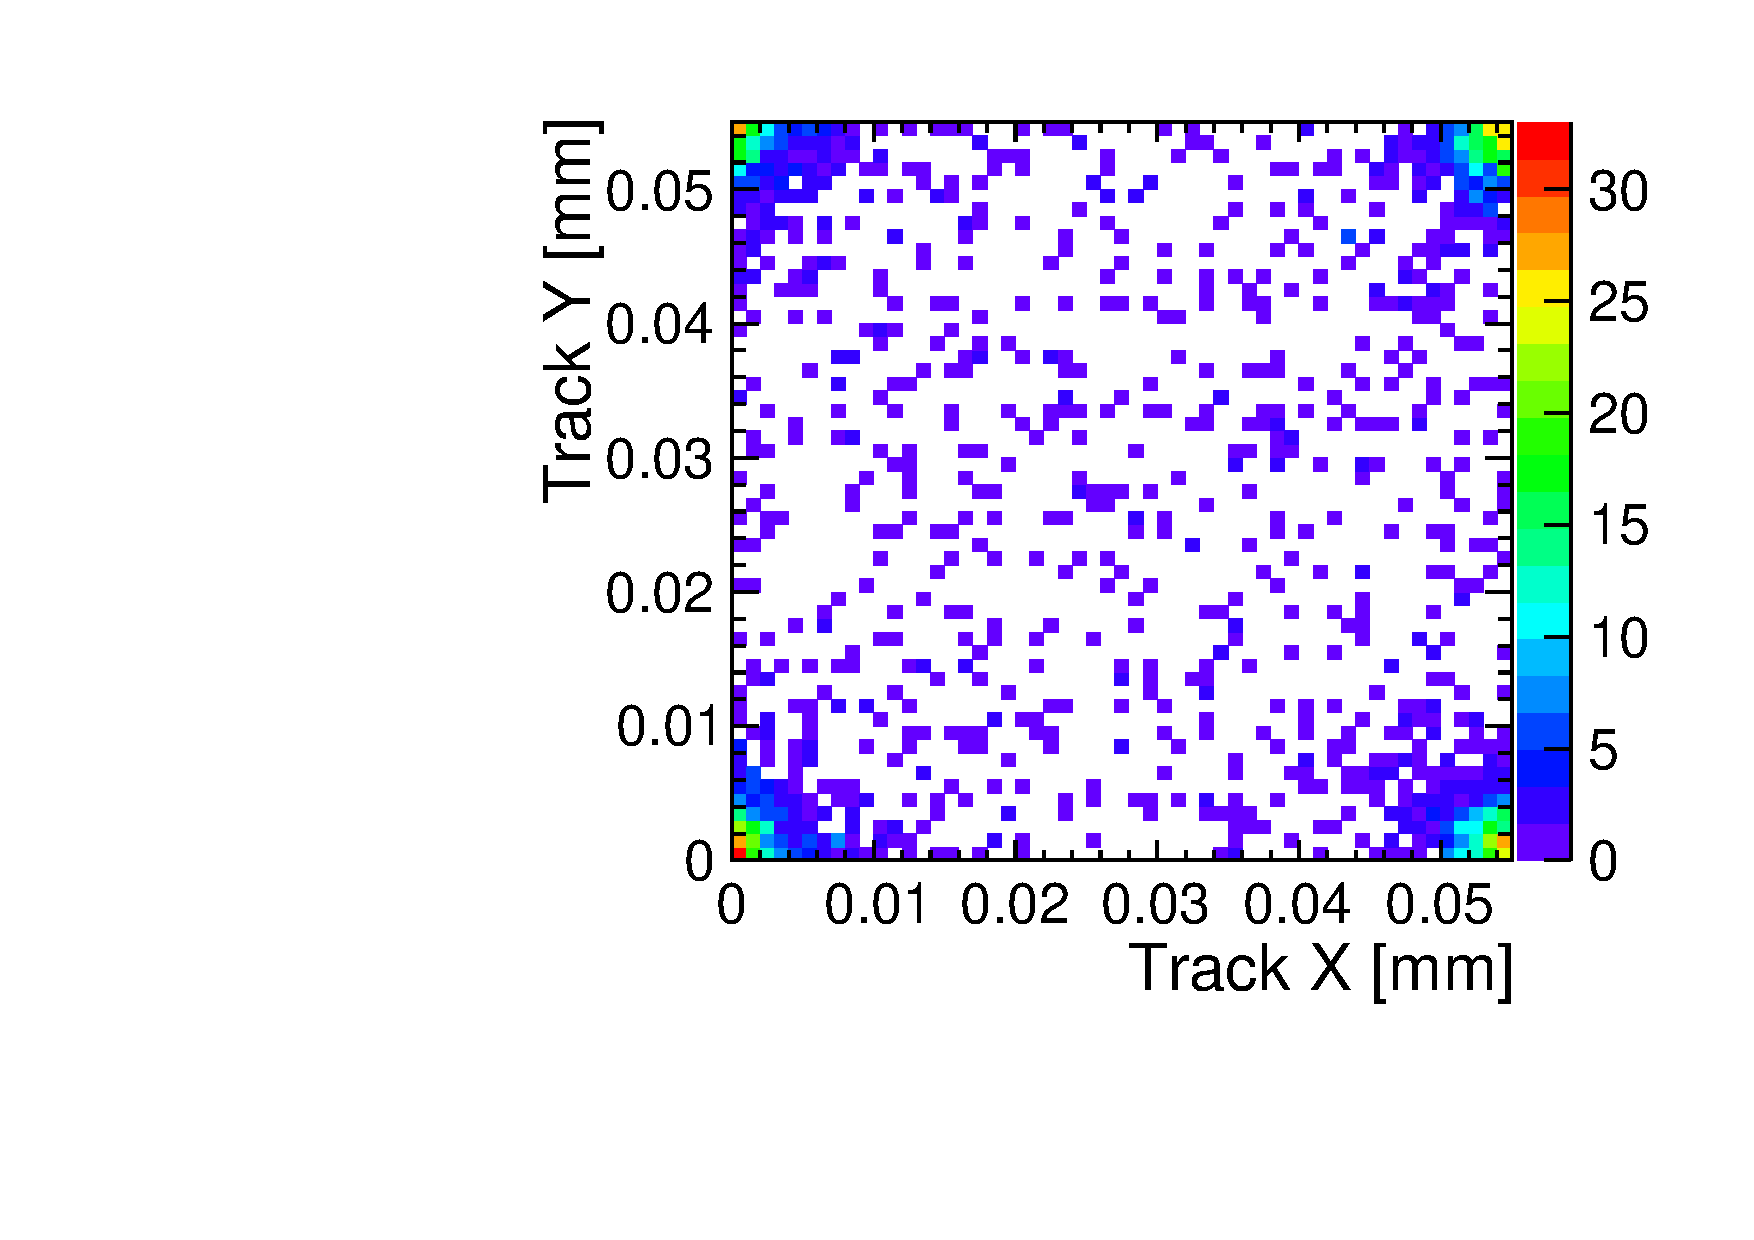
\includegraphics[width=\textwidth]{./figures/TestBeam/TrackPosWPixel_4hit_runW19_F7.pdf}
%     \caption{Cluster size 4}
%   \end{subfigure}
%   \caption{Extrapolated track position within the pixel for 1 to 4-hit
%     cluster sizes for a $50\,\micron$ sensor (assembly W19\_F7). The
%     assembly is operated at the nominal conditions.}
%   \label{fig:chargeSharingTrack_W19_F7}
% \end{figure}


% \begin{figure}[htbp] \centering
%   \begin{subfigure}[b]{0.23\textwidth}
%     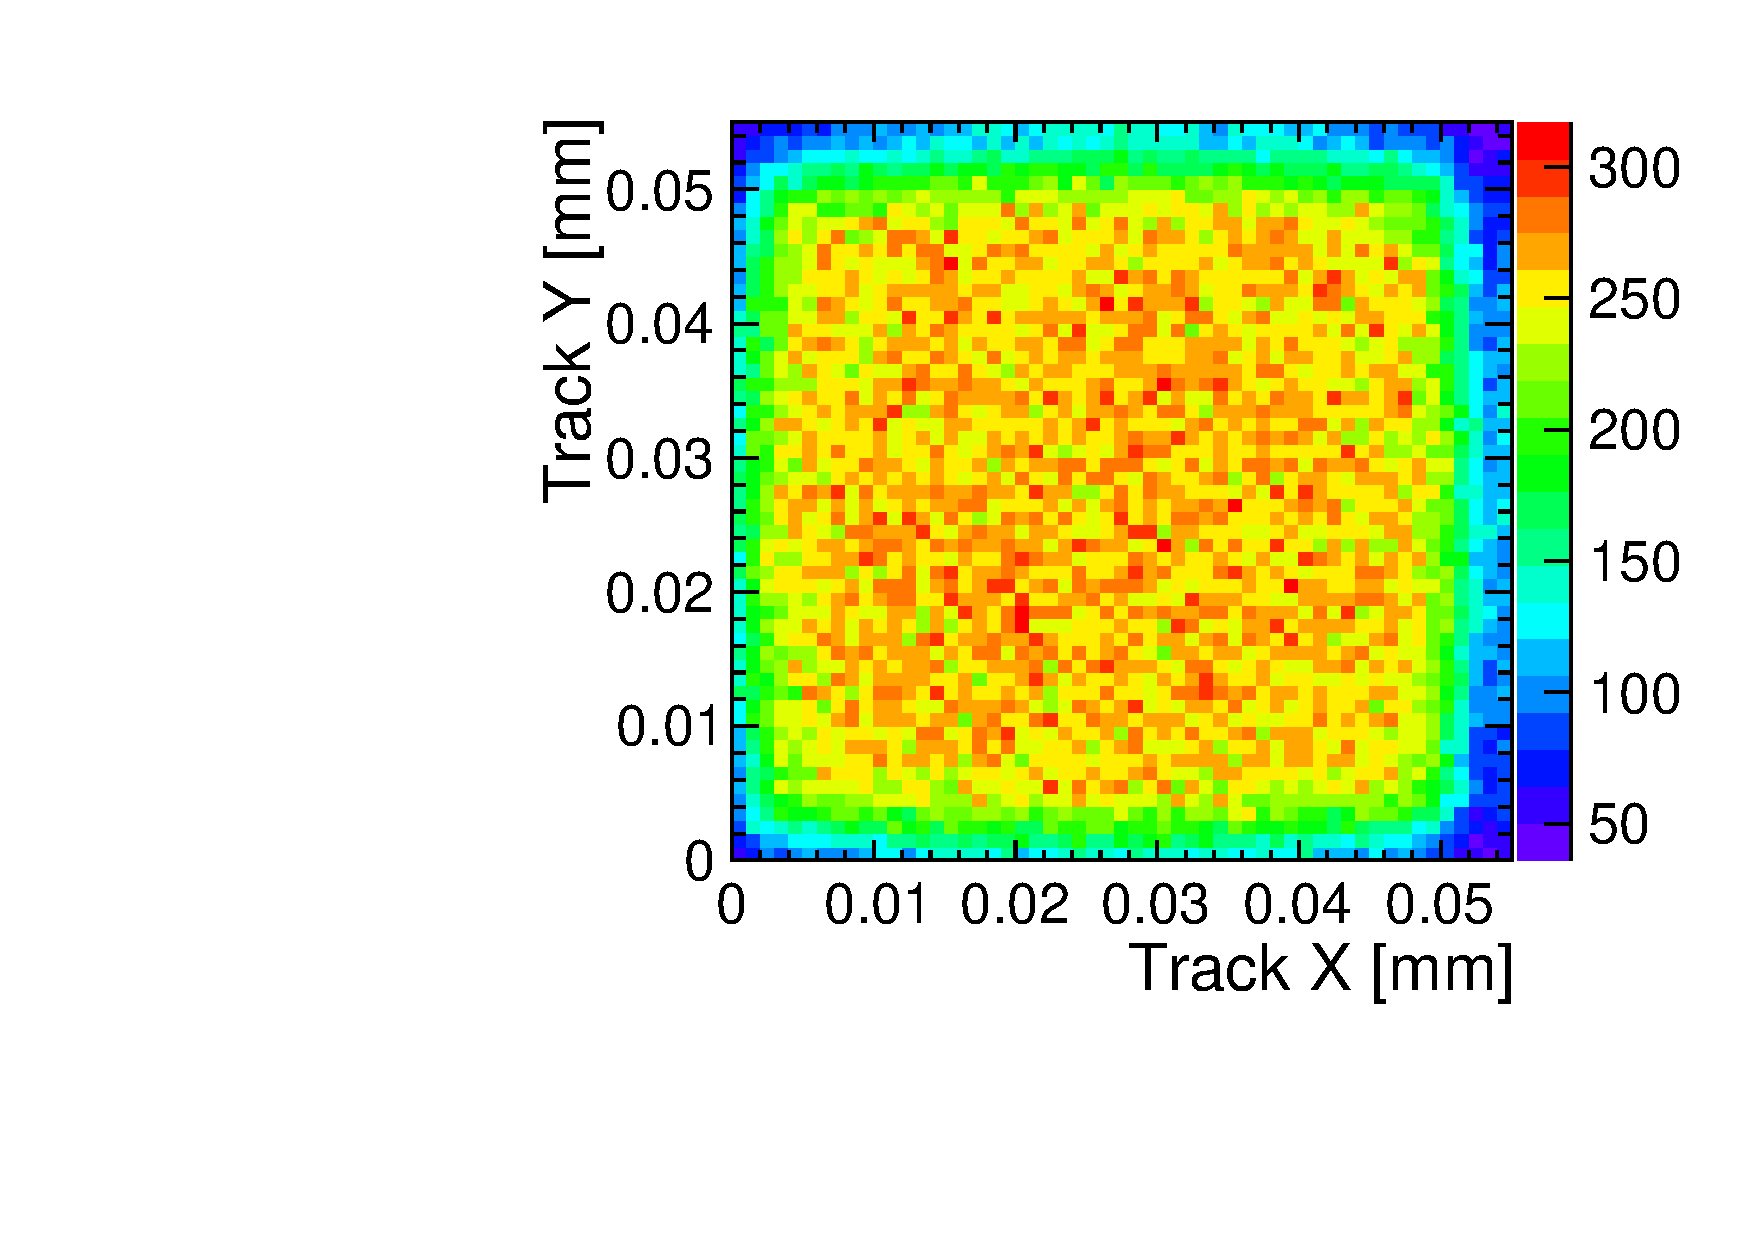
\includegraphics[width=\textwidth]{./figures/TestBeam/TrackPosWPixel_1hit_runW19_L8.pdf}
%     \caption{Cluster size 1}
%   \end{subfigure} \hfill
%   \begin{subfigure}[b]{0.23\textwidth}
%     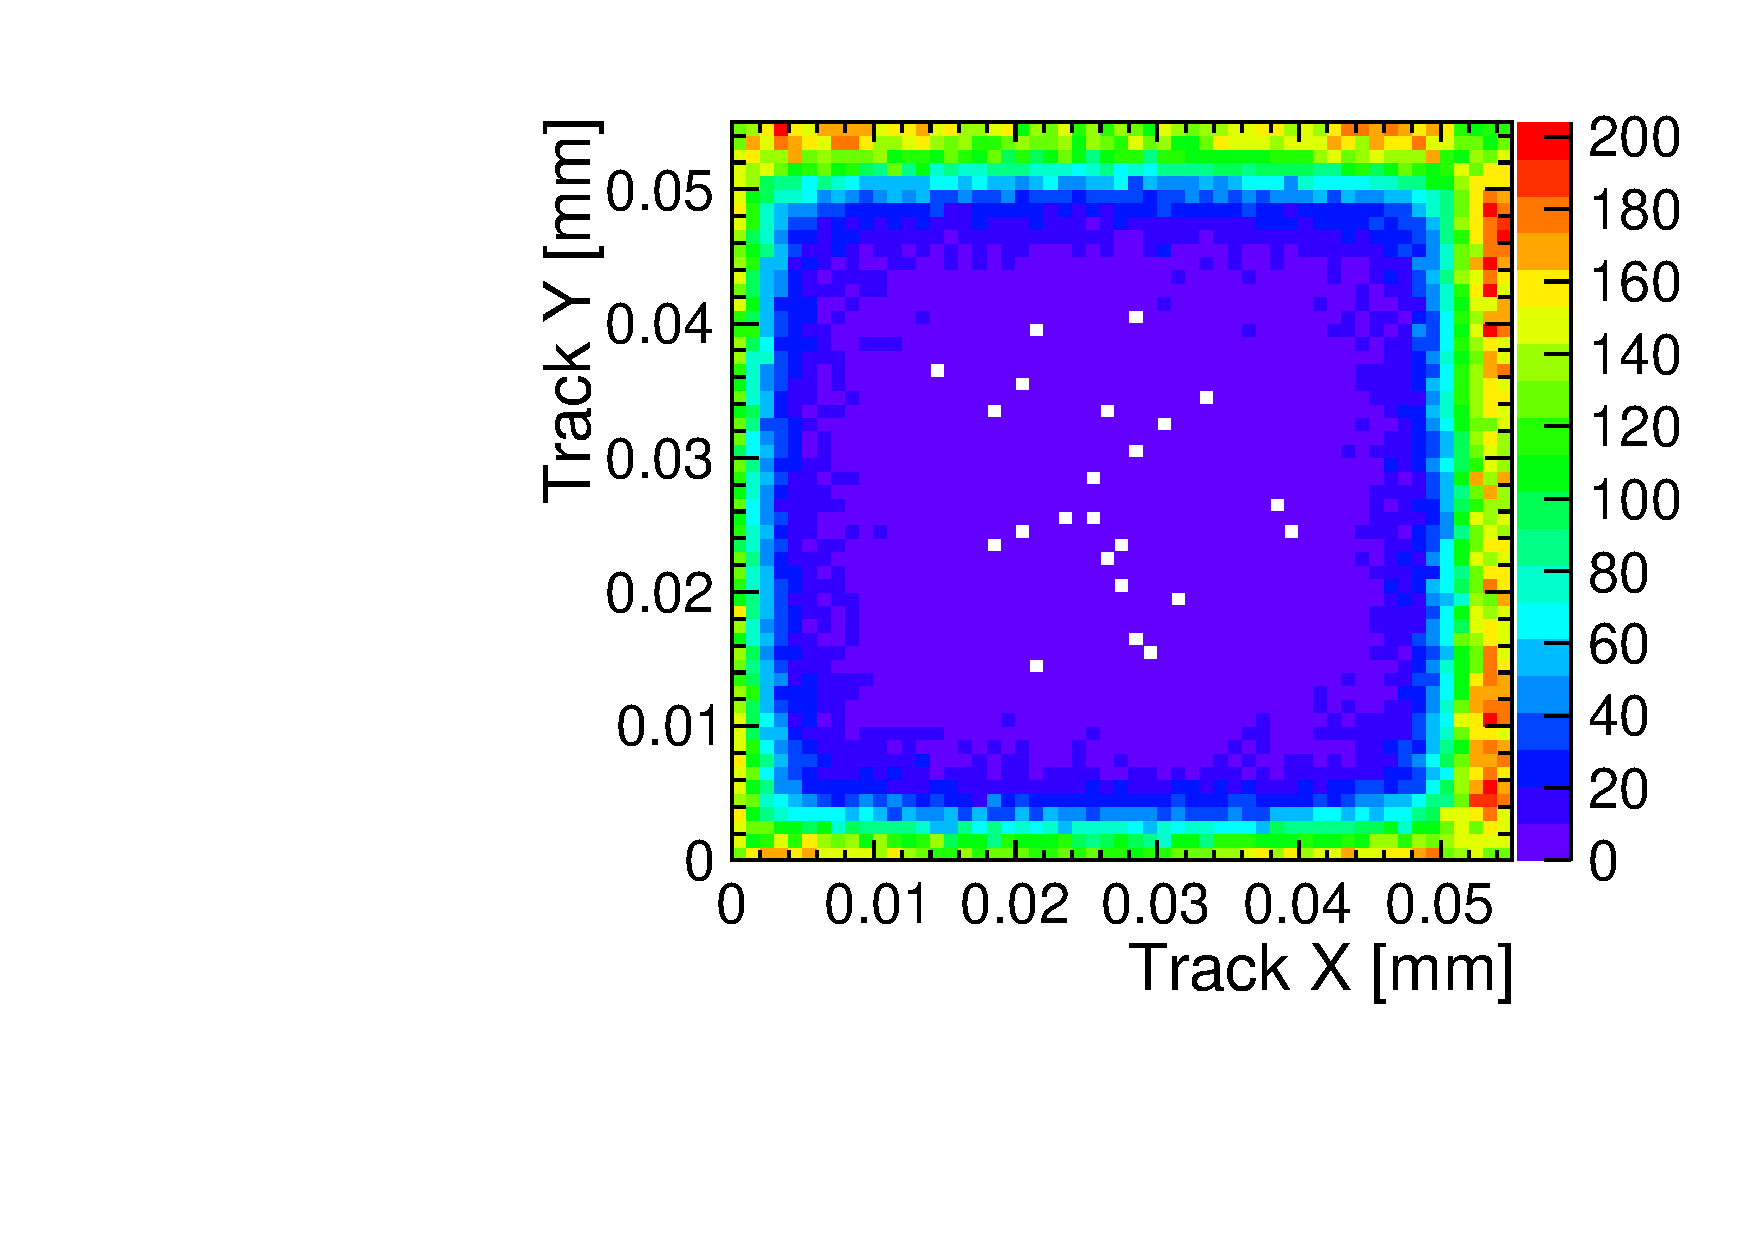
\includegraphics[width=\textwidth]{./figures/TestBeam/TrackPosWPixel_2hit_runW19_L8.pdf}
%     \caption{Cluster size 2}
%   \end{subfigure} \hfill
%   \begin{subfigure}[b]{0.23\textwidth}
%     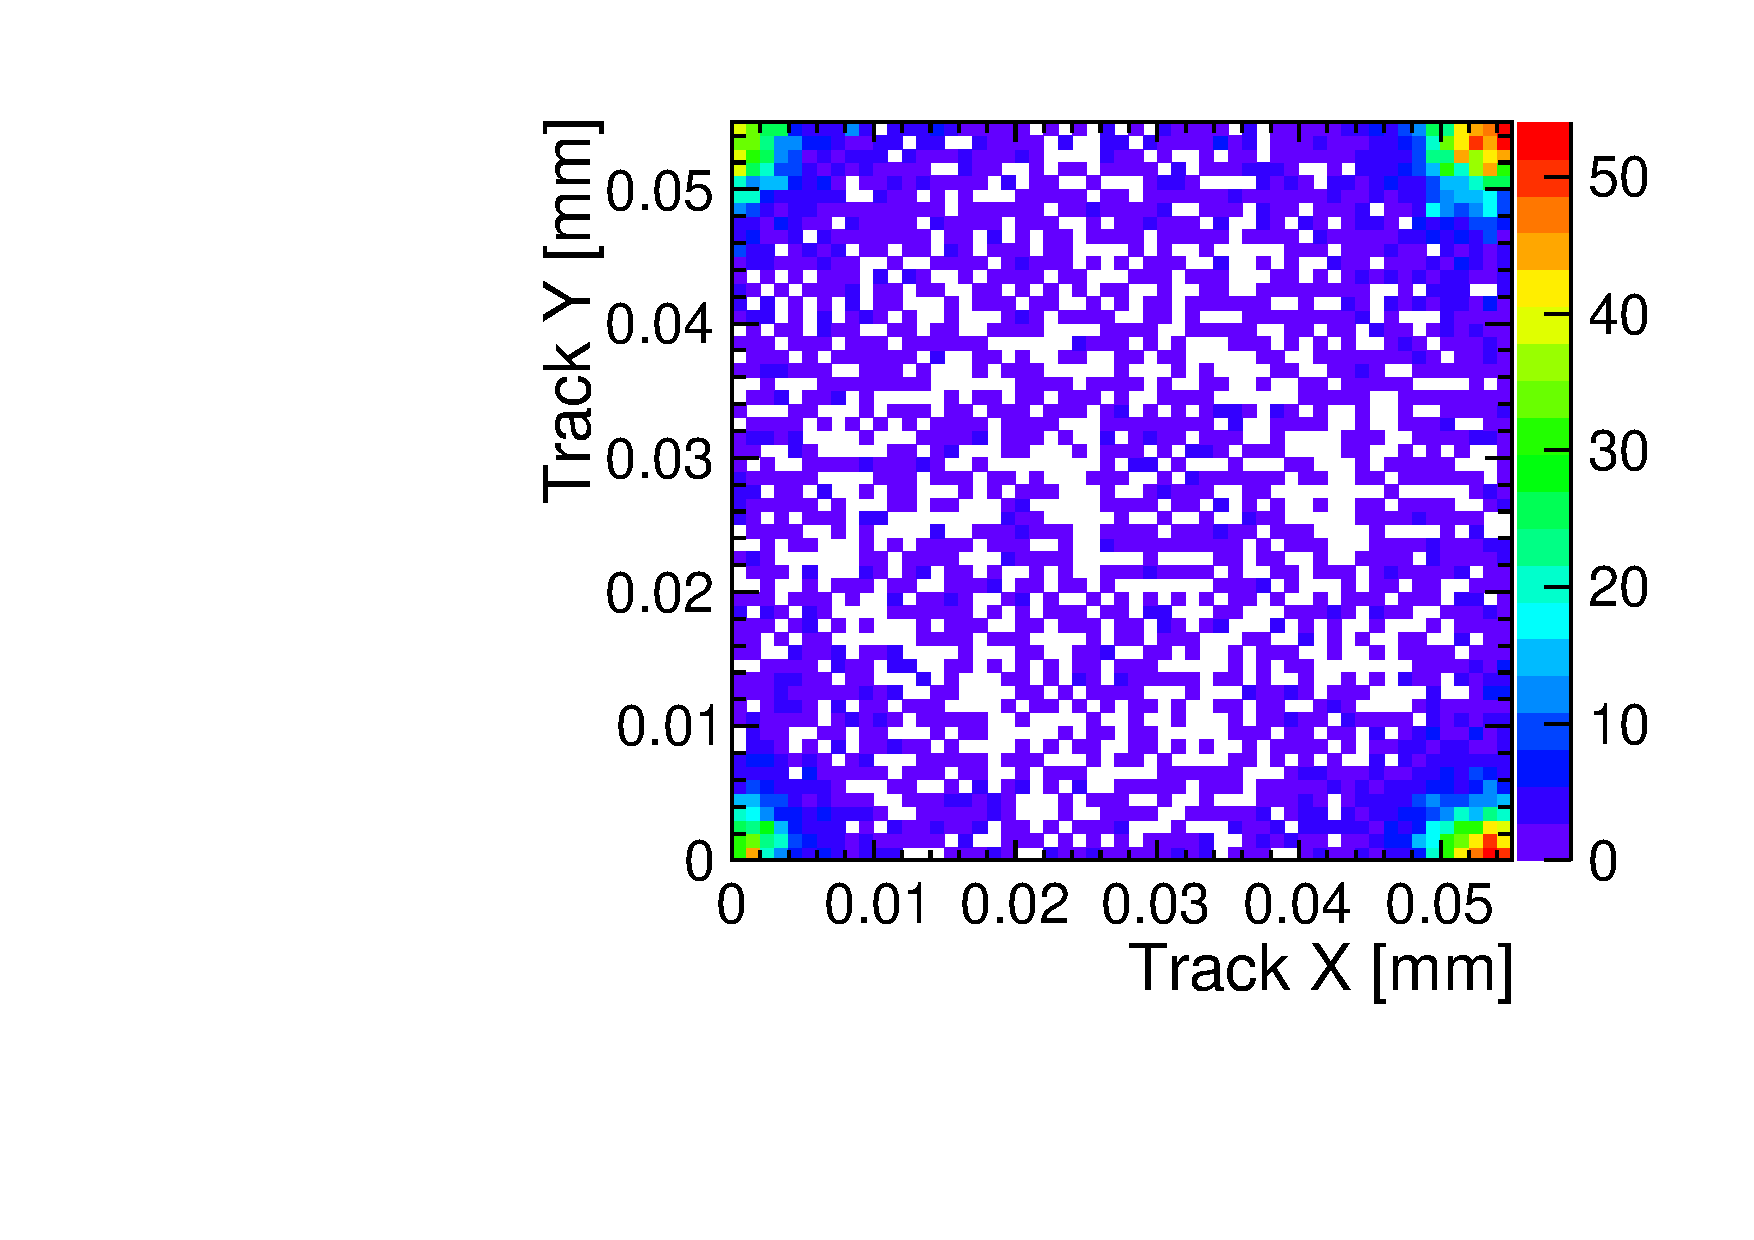
\includegraphics[width=\textwidth]{./figures/TestBeam/TrackPosWPixel_3hit_runW19_L8.pdf}
%     \caption{Cluster size 3}
%   \end{subfigure} \hfill
%   \begin{subfigure}[b]{0.23\textwidth}
%     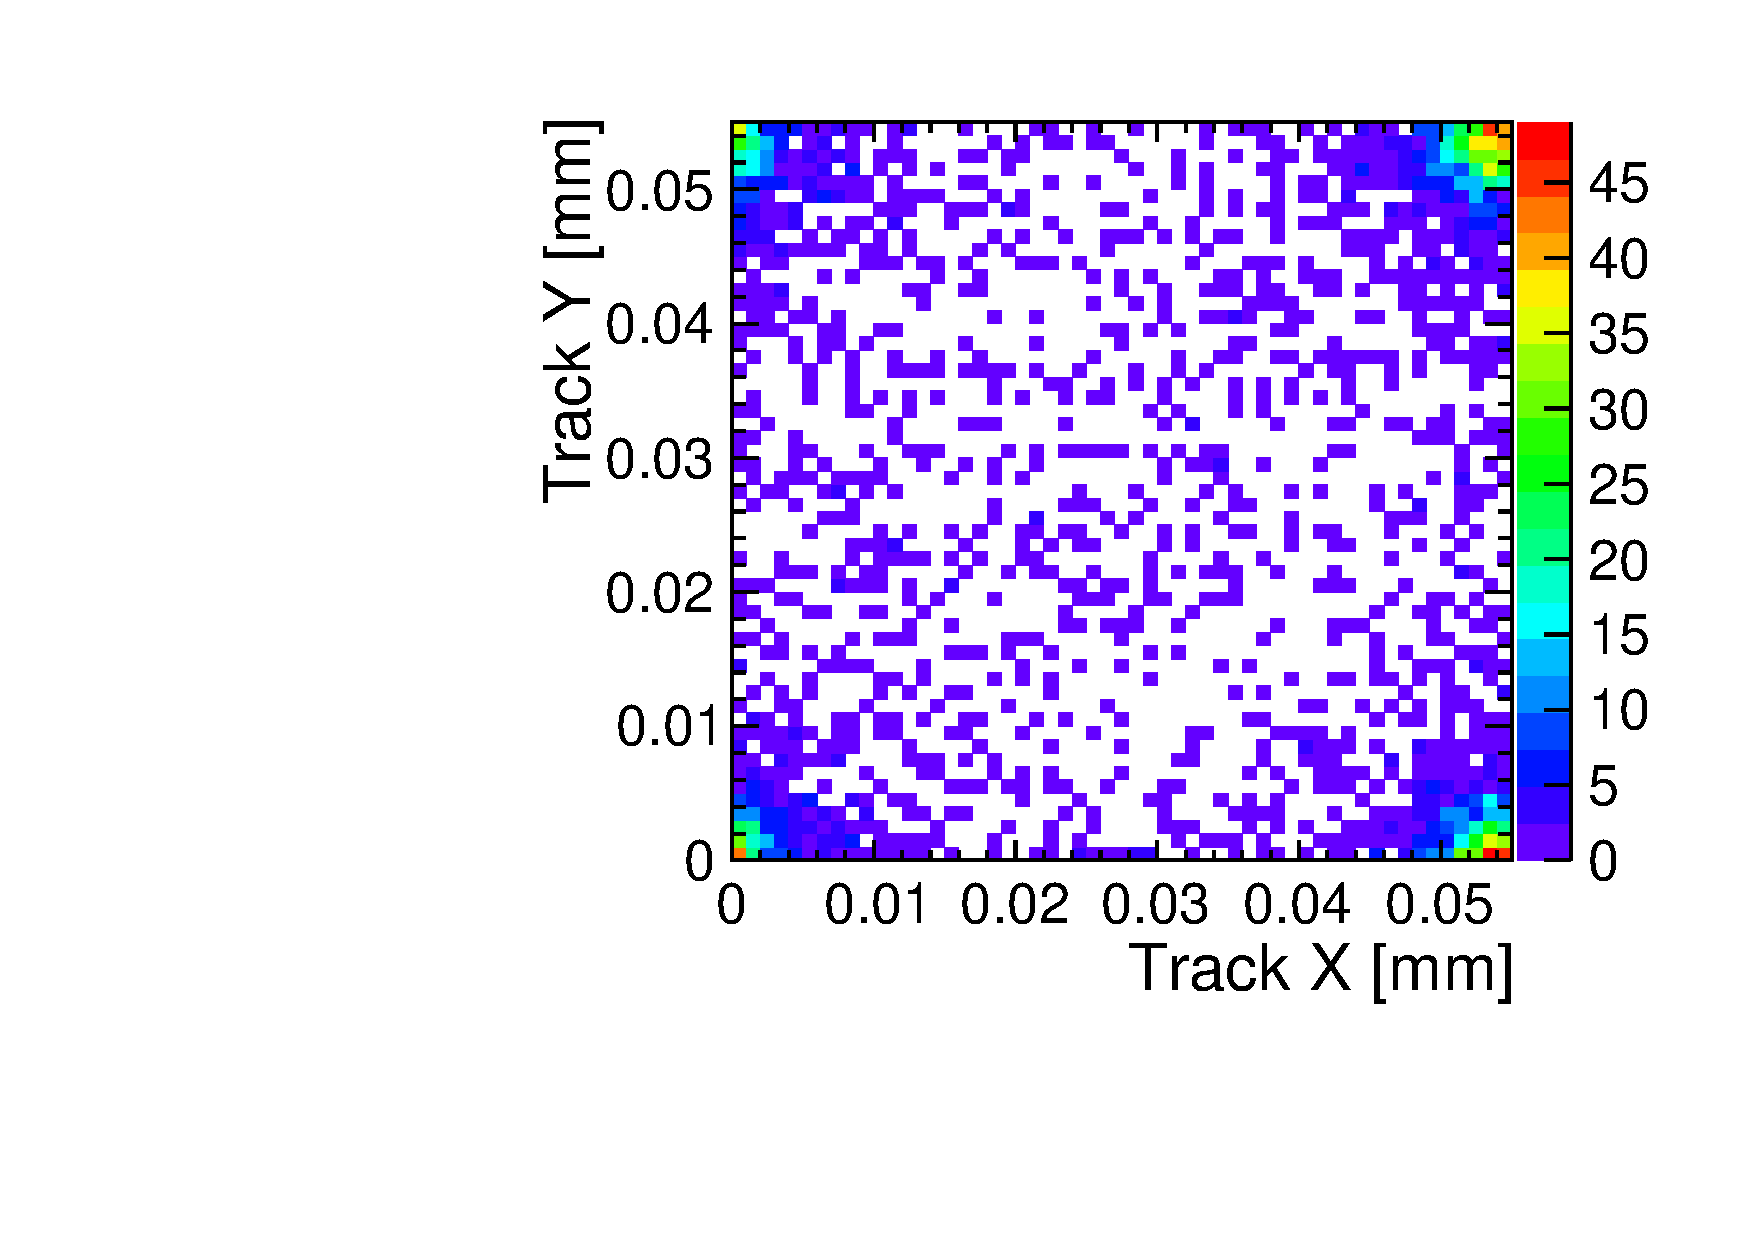
\includegraphics[width=\textwidth]{./figures/TestBeam/TrackPosWPixel_4hit_runW19_L8.pdf}
%     \caption{Cluster size 4}
%   \end{subfigure}
%   \caption{Extrapolated track position within the pixel for 1 to 4-hit
%     cluster sizes for a $50\,\micron$ sensor (assembly W19\_L8). The
%     assembly is operated at the nominal conditions.}
%   \label{fig:chargeSharingTrack_W19_L8}
% \end{figure}



% \newpage
% %% --------------------------------------------- %%
% \section{Residuals}
% \subsection{Residuals vs. bias voltage}
% \begin{figure}[htbp] \centering
%   \begin{subfigure}[b]{0.33\textwidth}
%     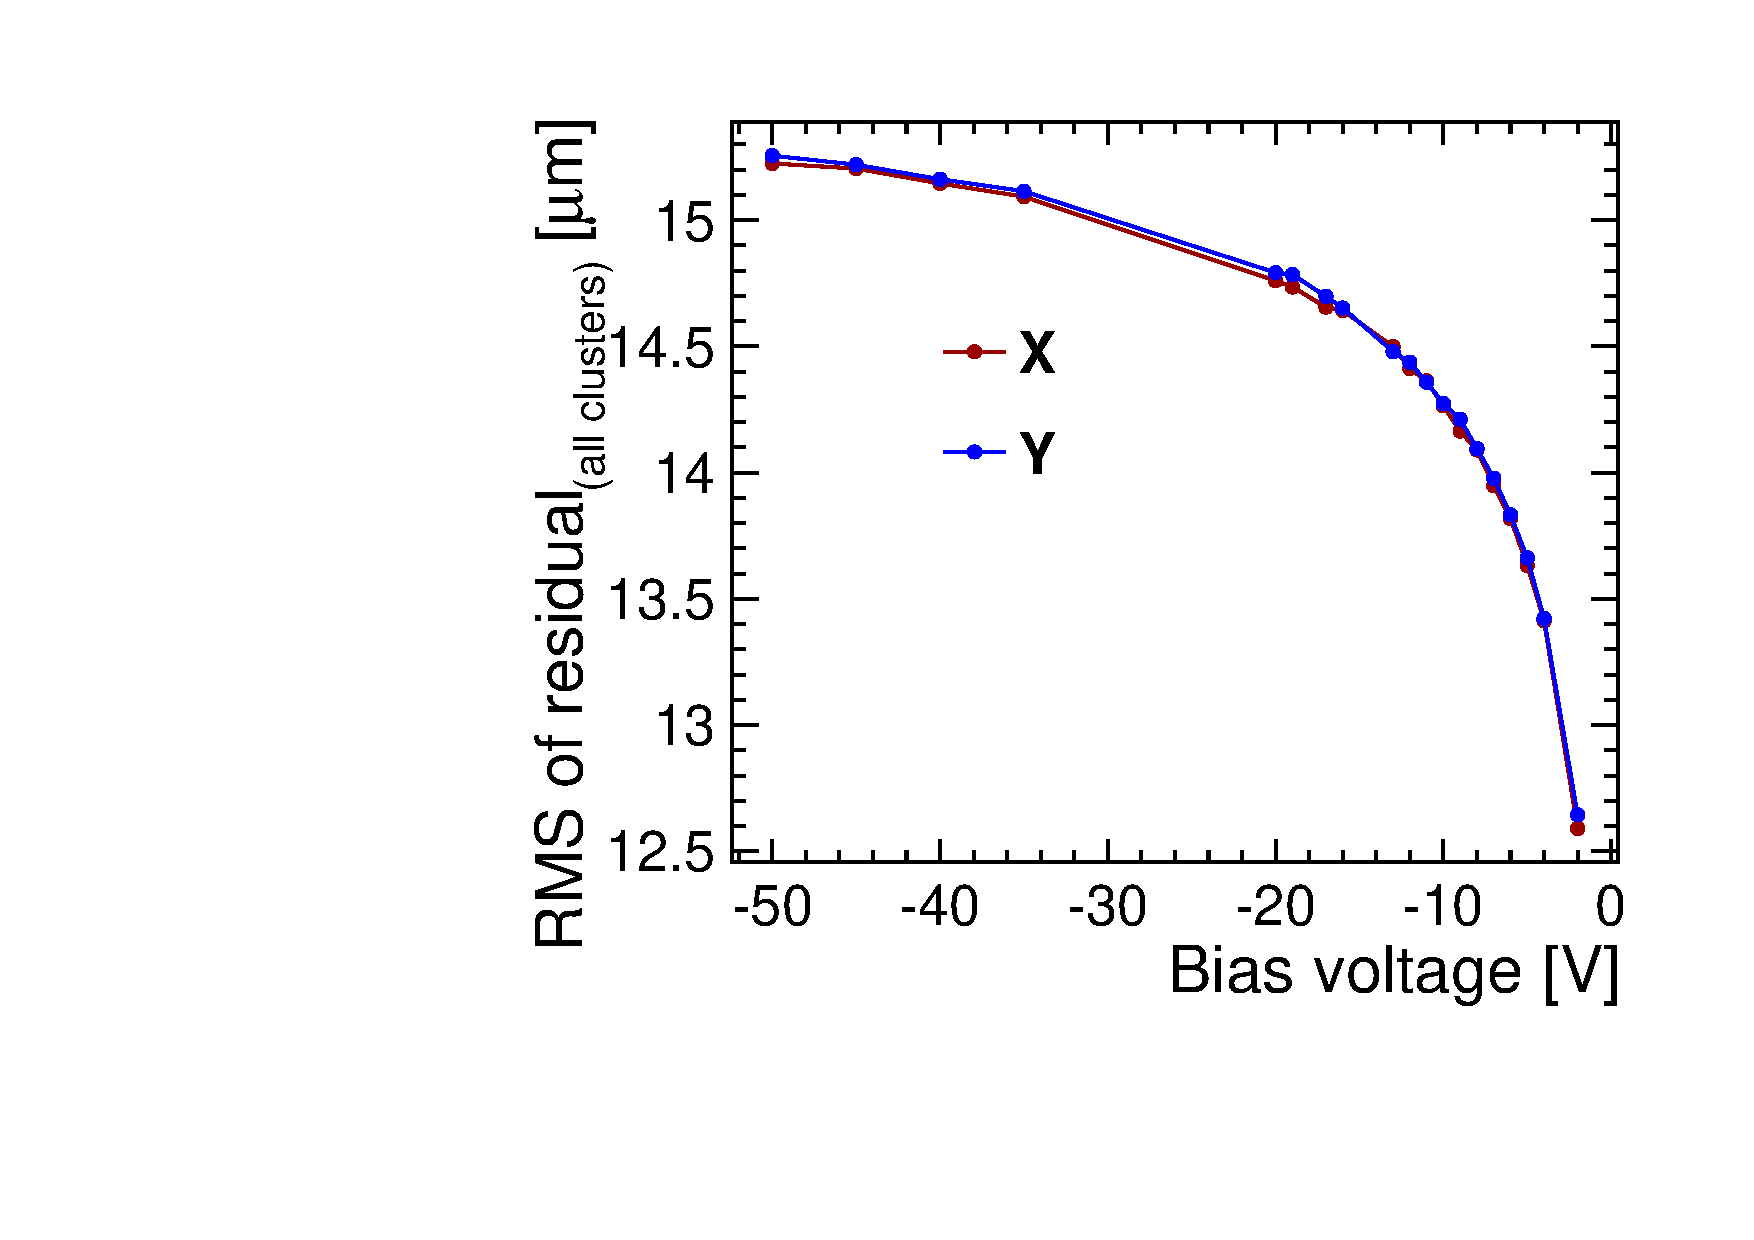
\includegraphics[width=\textwidth]{./figures/TestBeam/W19_G7_Residual_vs_bias.pdf}
%     \caption{20-NGR}
%   \end{subfigure} \hfill
%   \begin{subfigure}[b]{0.33\textwidth}
%     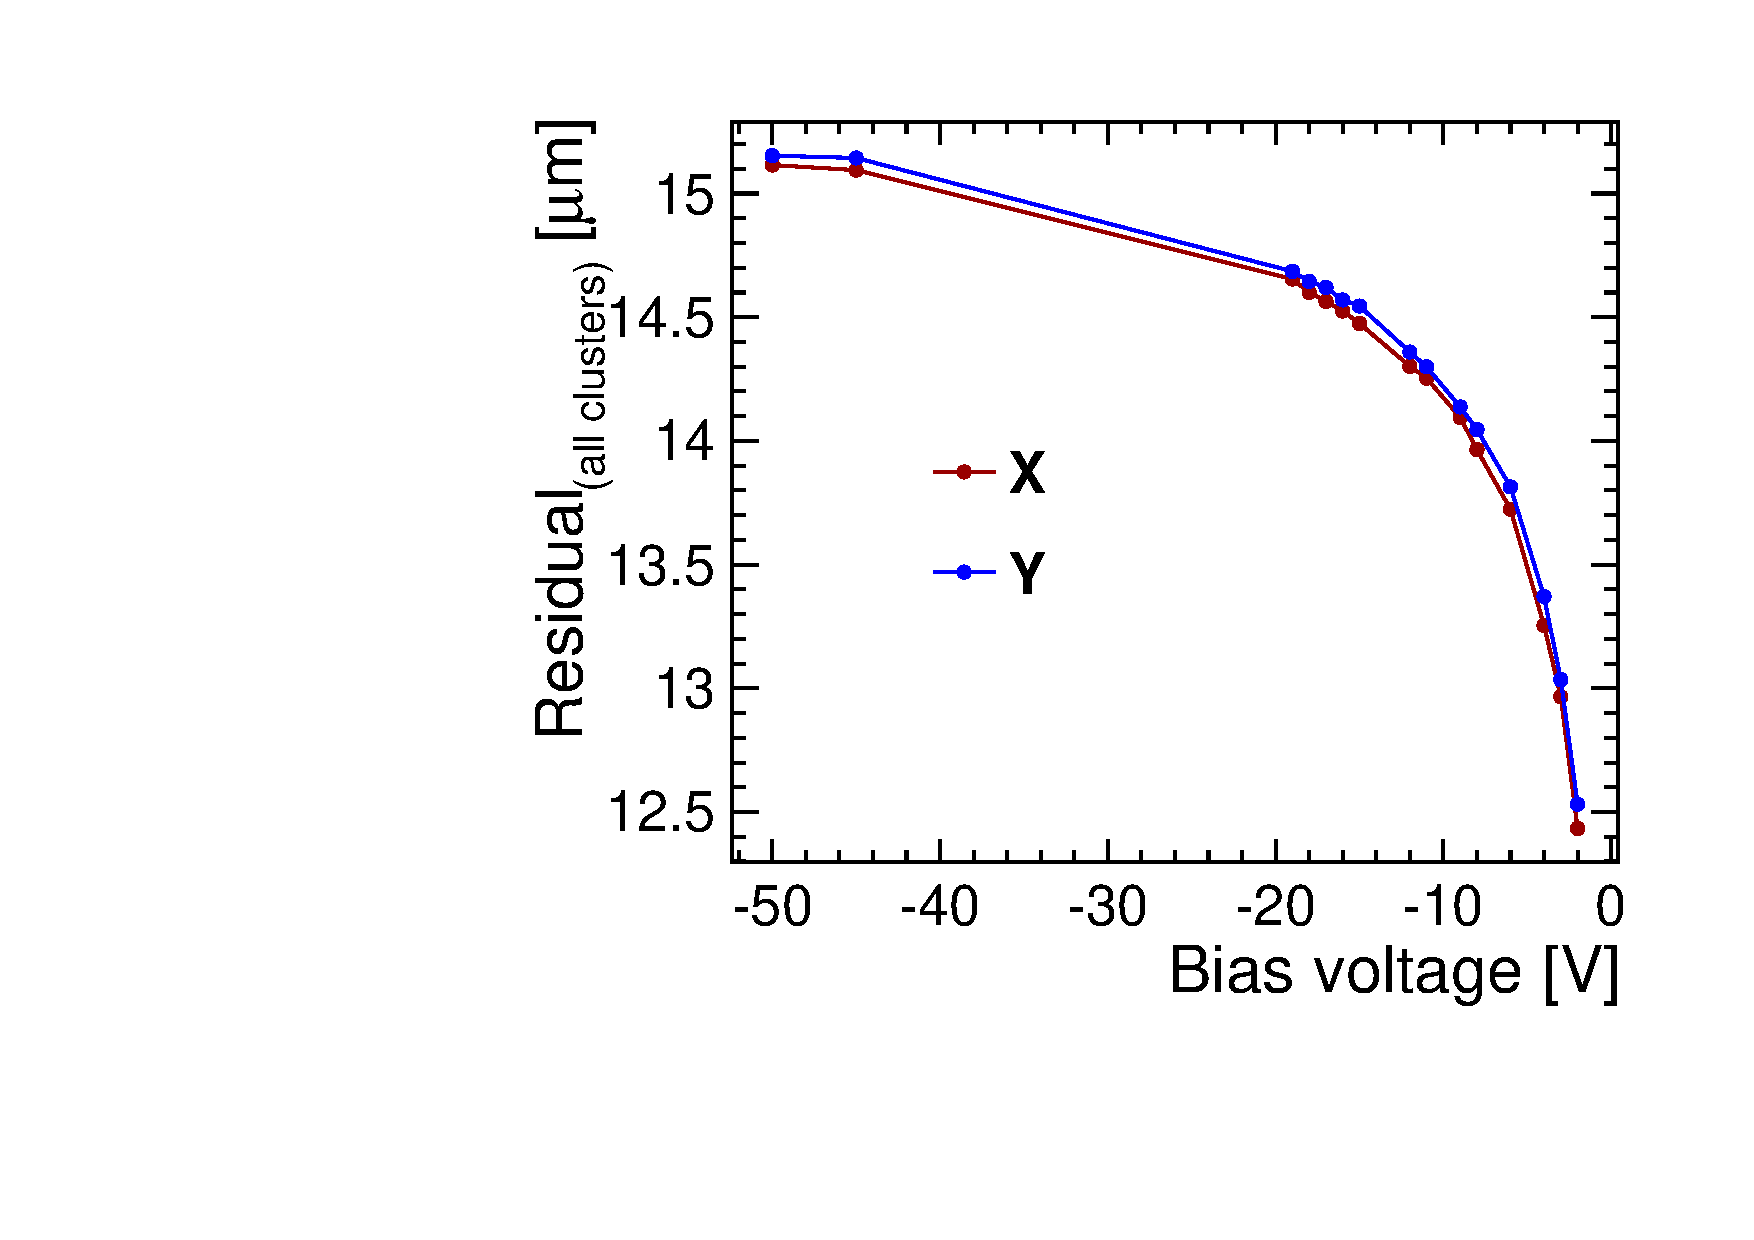
\includegraphics[width=\textwidth]{./figures/TestBeam/W19_F7_Residual_vs_bias.pdf}
%     \caption{23-FGR}
%   \end{subfigure}\hfill
%   \begin{subfigure}[b]{0.33\textwidth}
%     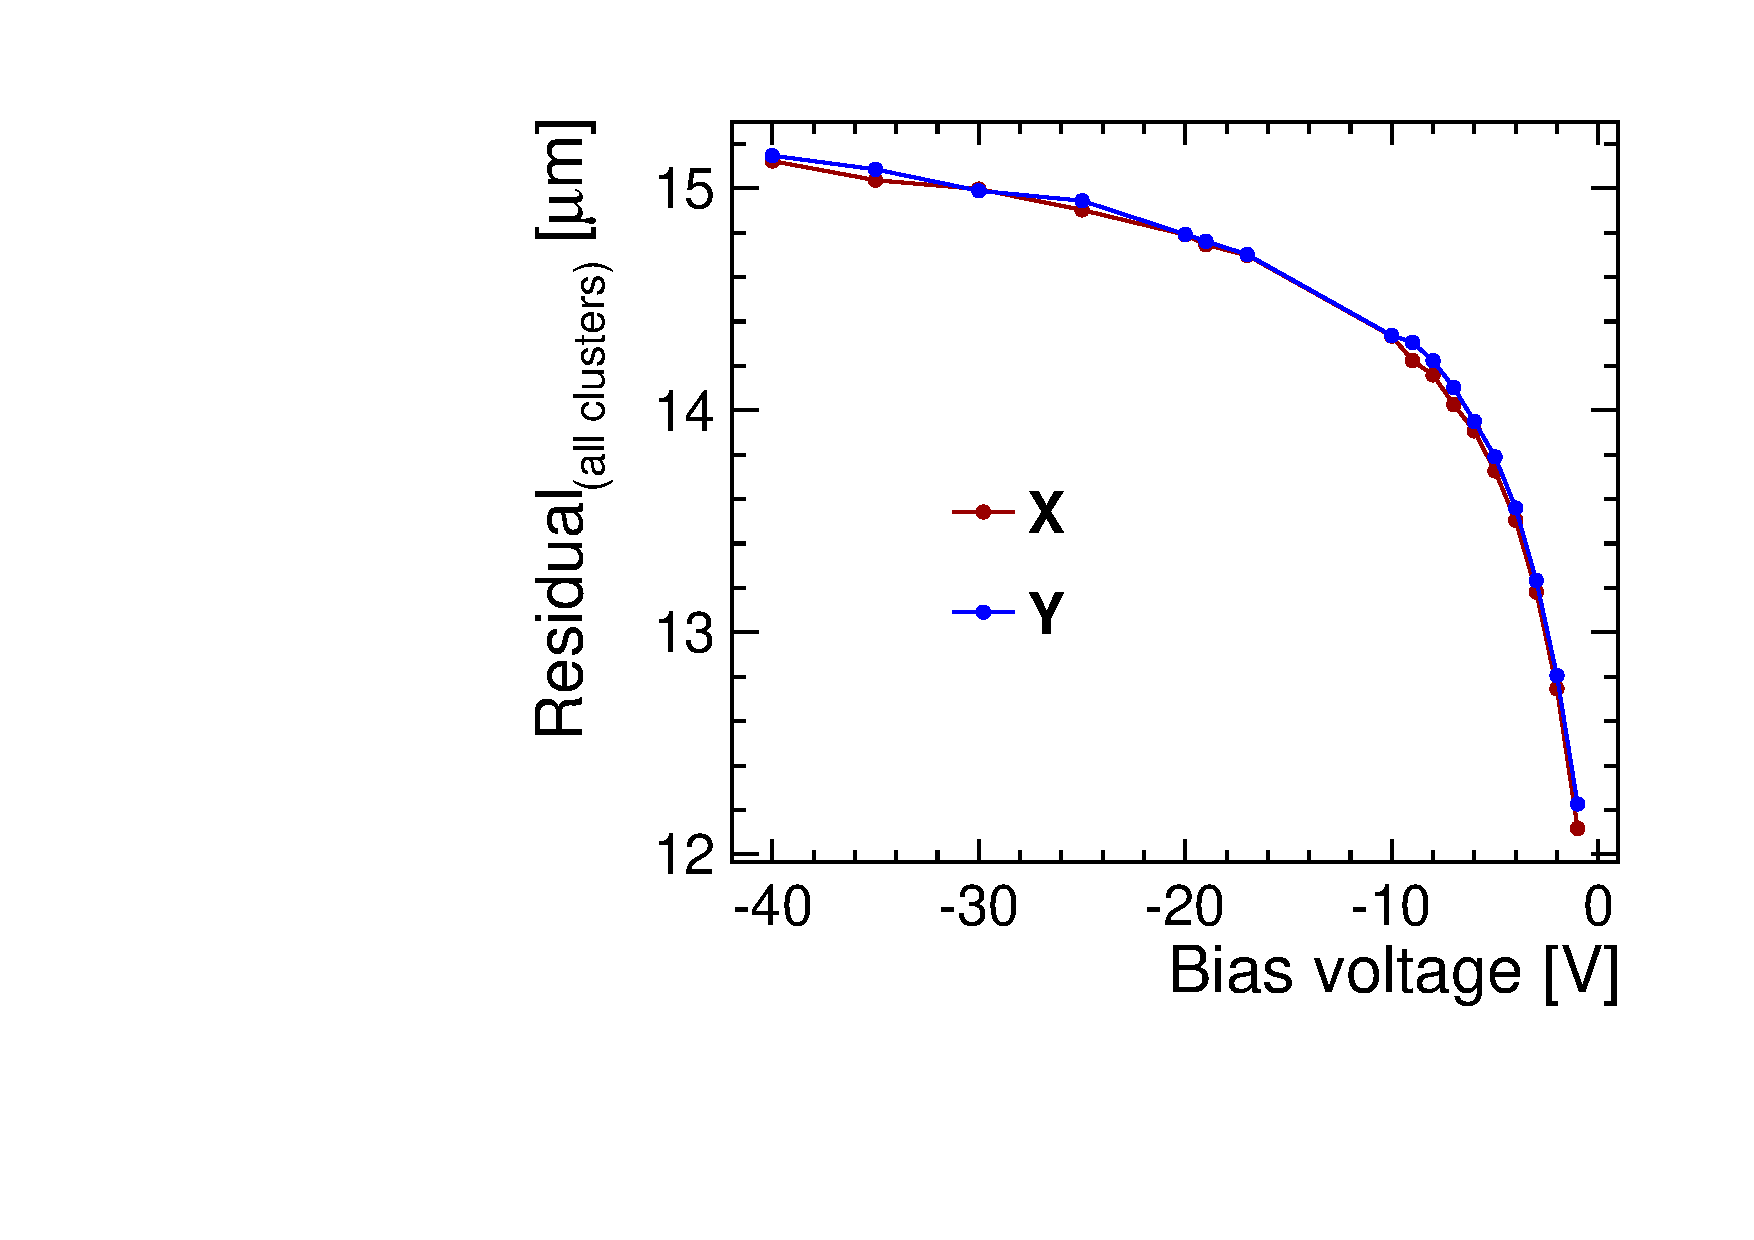
\includegraphics[width=\textwidth]{./figures/TestBeam/W19_L8_Residual_vs_bias.pdf}
%     \caption{28-GNDGR}
%   \end{subfigure} \\

%   \begin{subfigure}[b]{0.33\textwidth}
%     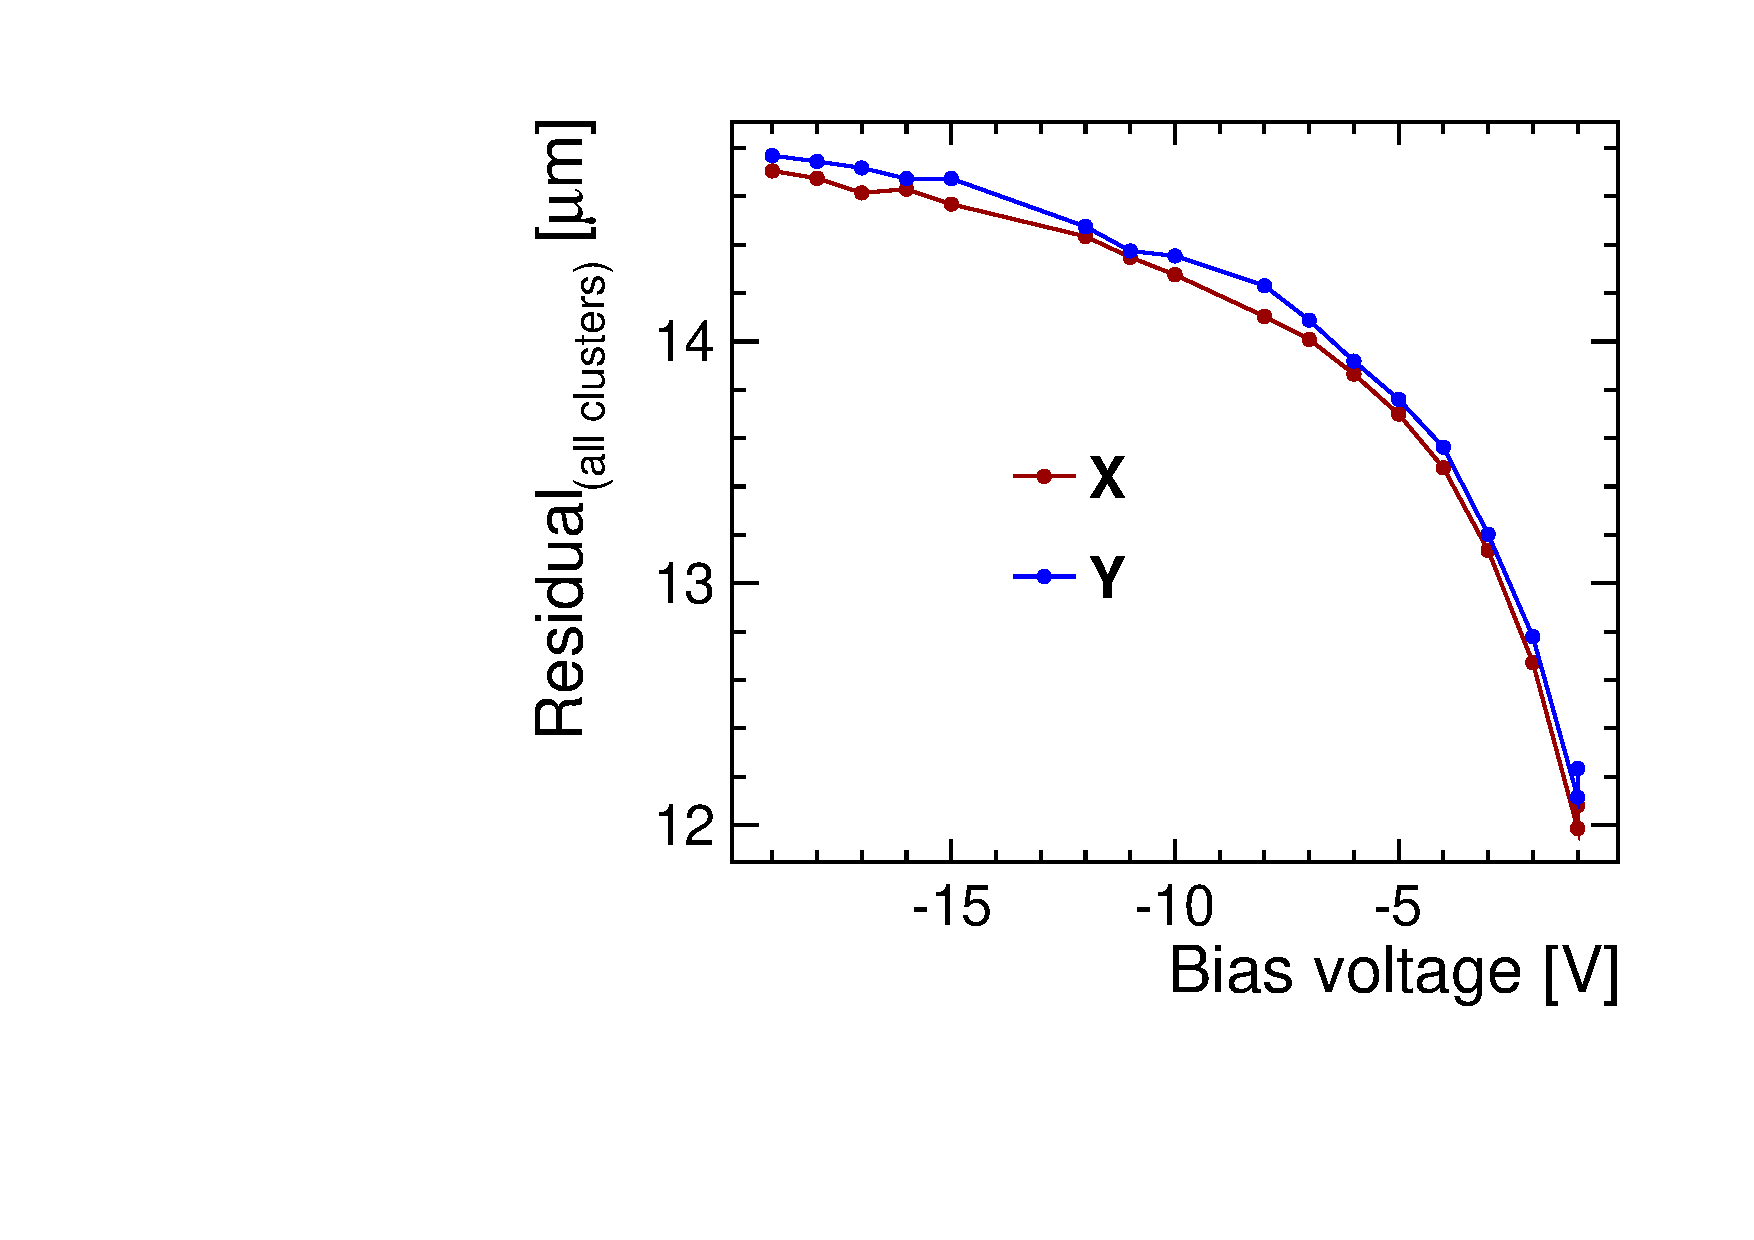
\includegraphics[width=\textwidth]{./figures/TestBeam/W19_C7_Residual_vs_bias.pdf}
%     \caption{55-GNDGR}
%   \end{subfigure} \hfill
%   \begin{subfigure}[b]{0.33\textwidth}
%     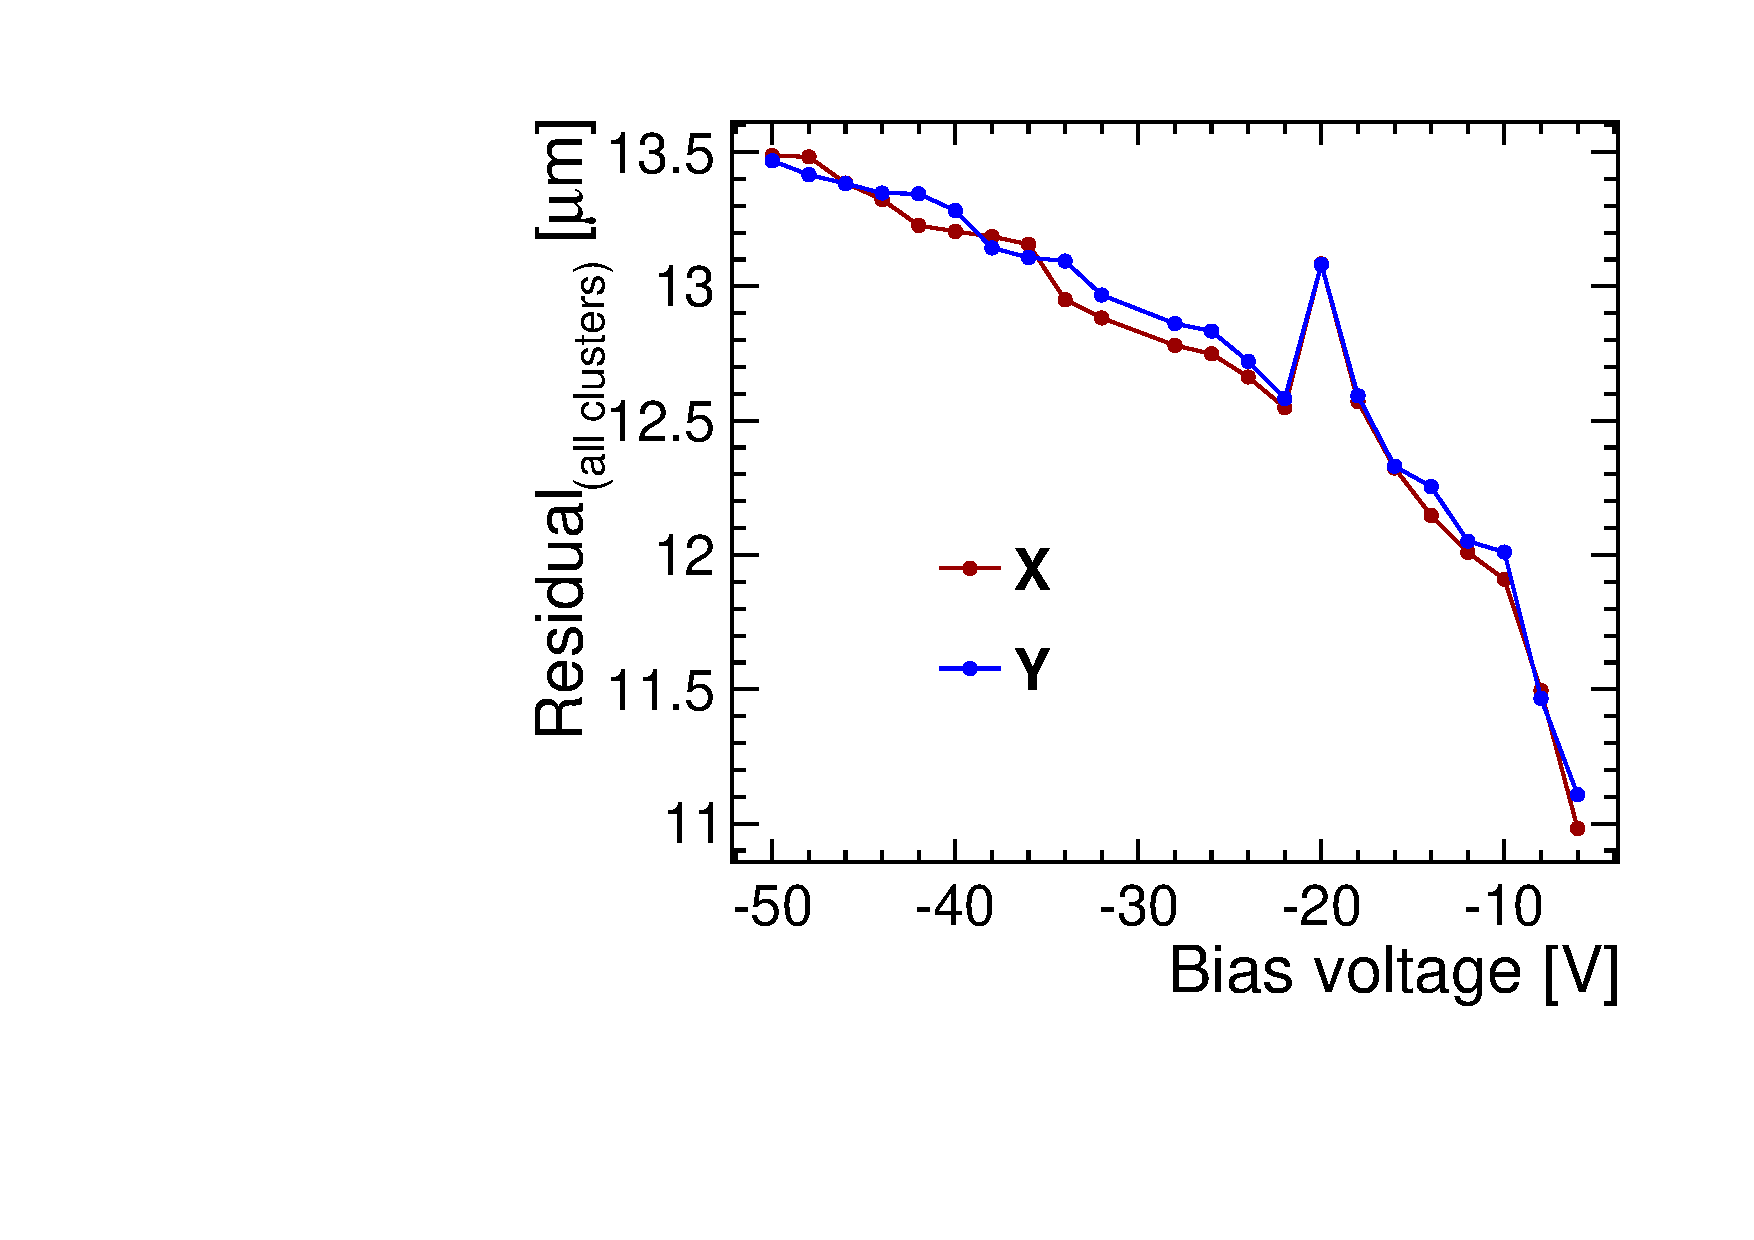
\includegraphics[width=\textwidth]{./figures/TestBeam/W5_E2_Residual_vs_bias.pdf}
%     \caption{55-GND-GR-100}
%   \end{subfigure}\hfill
%   \begin{subfigure}[b]{0.33\textwidth}
%     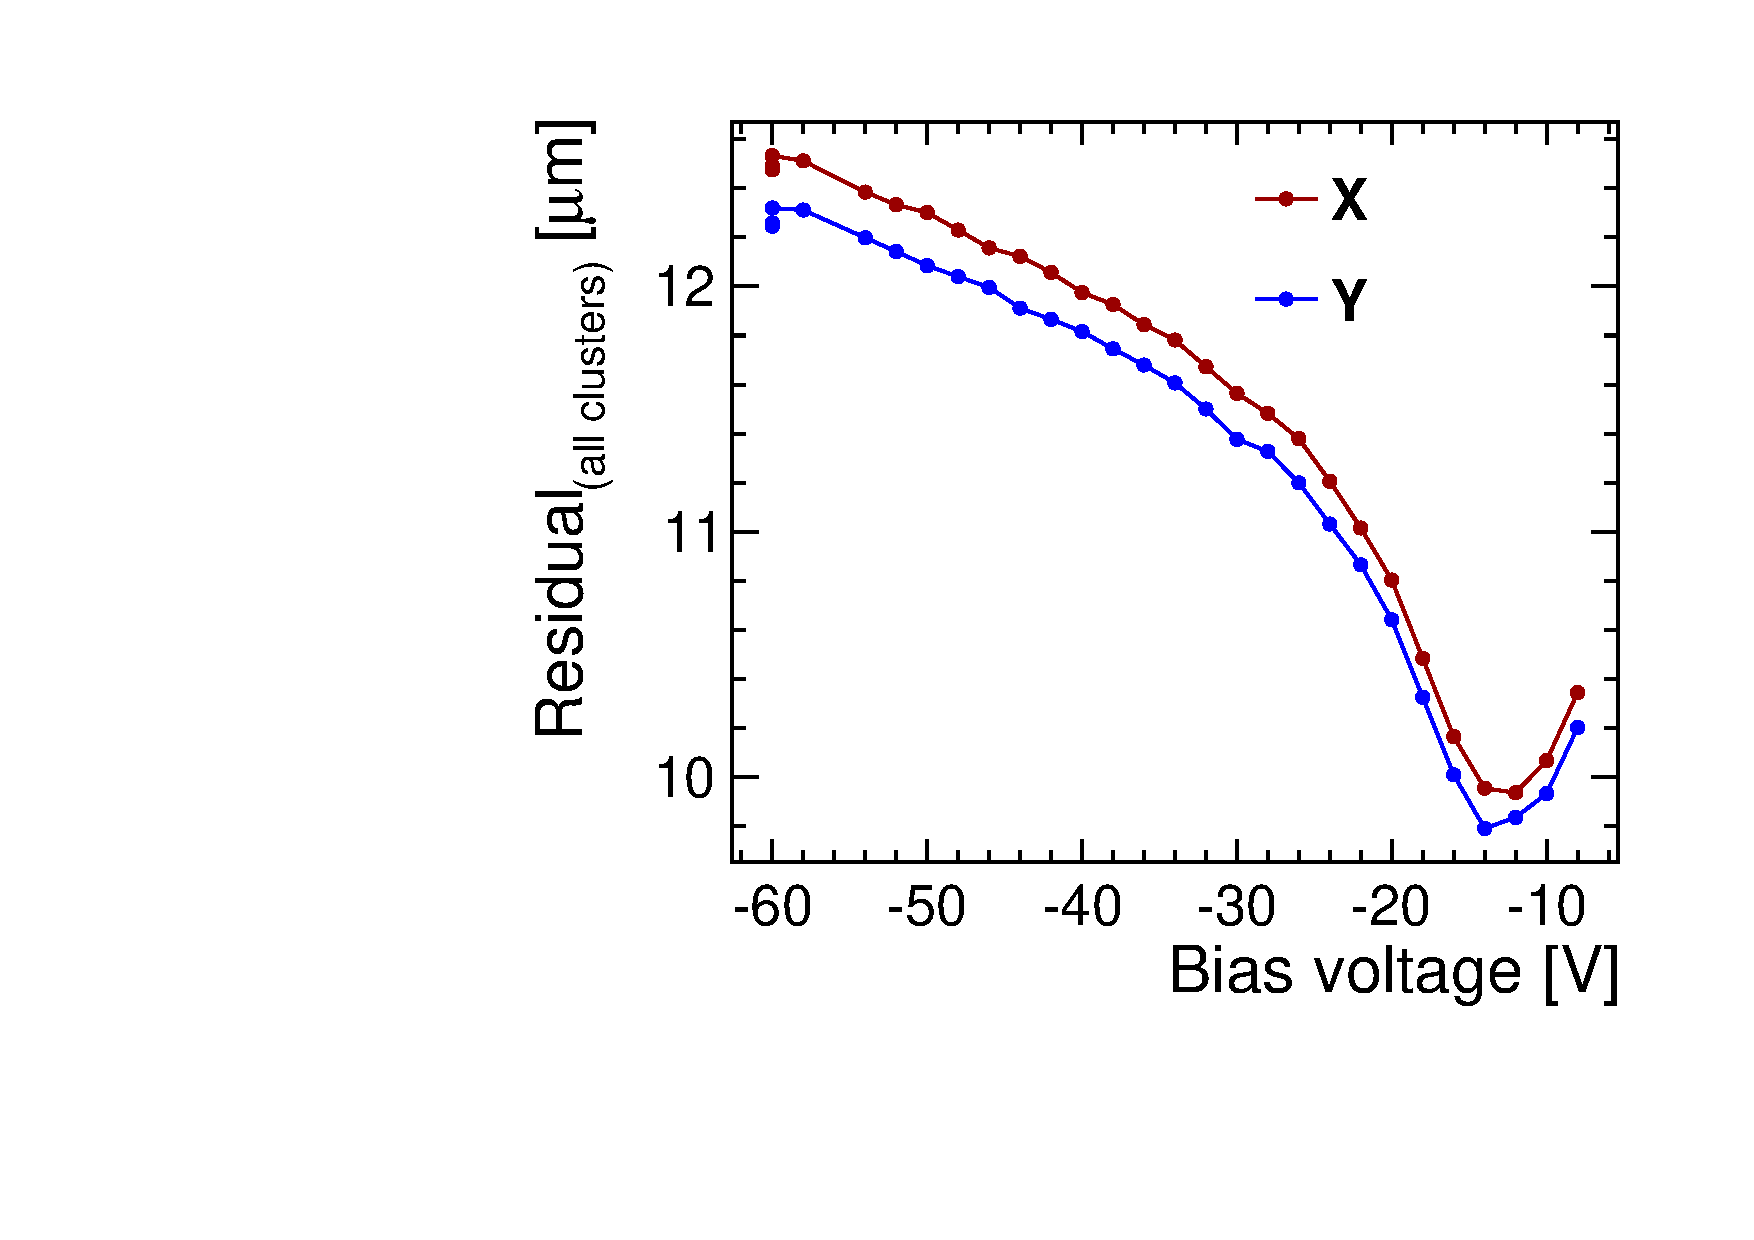
\includegraphics[width=\textwidth]{./figures/TestBeam/W5_F1_Residual_vs_bias.pdf}
%     \caption{55-GND-GR-150}
%   \end{subfigure}\\
%   \begin{subfigure}[b]{0.33\textwidth}
%     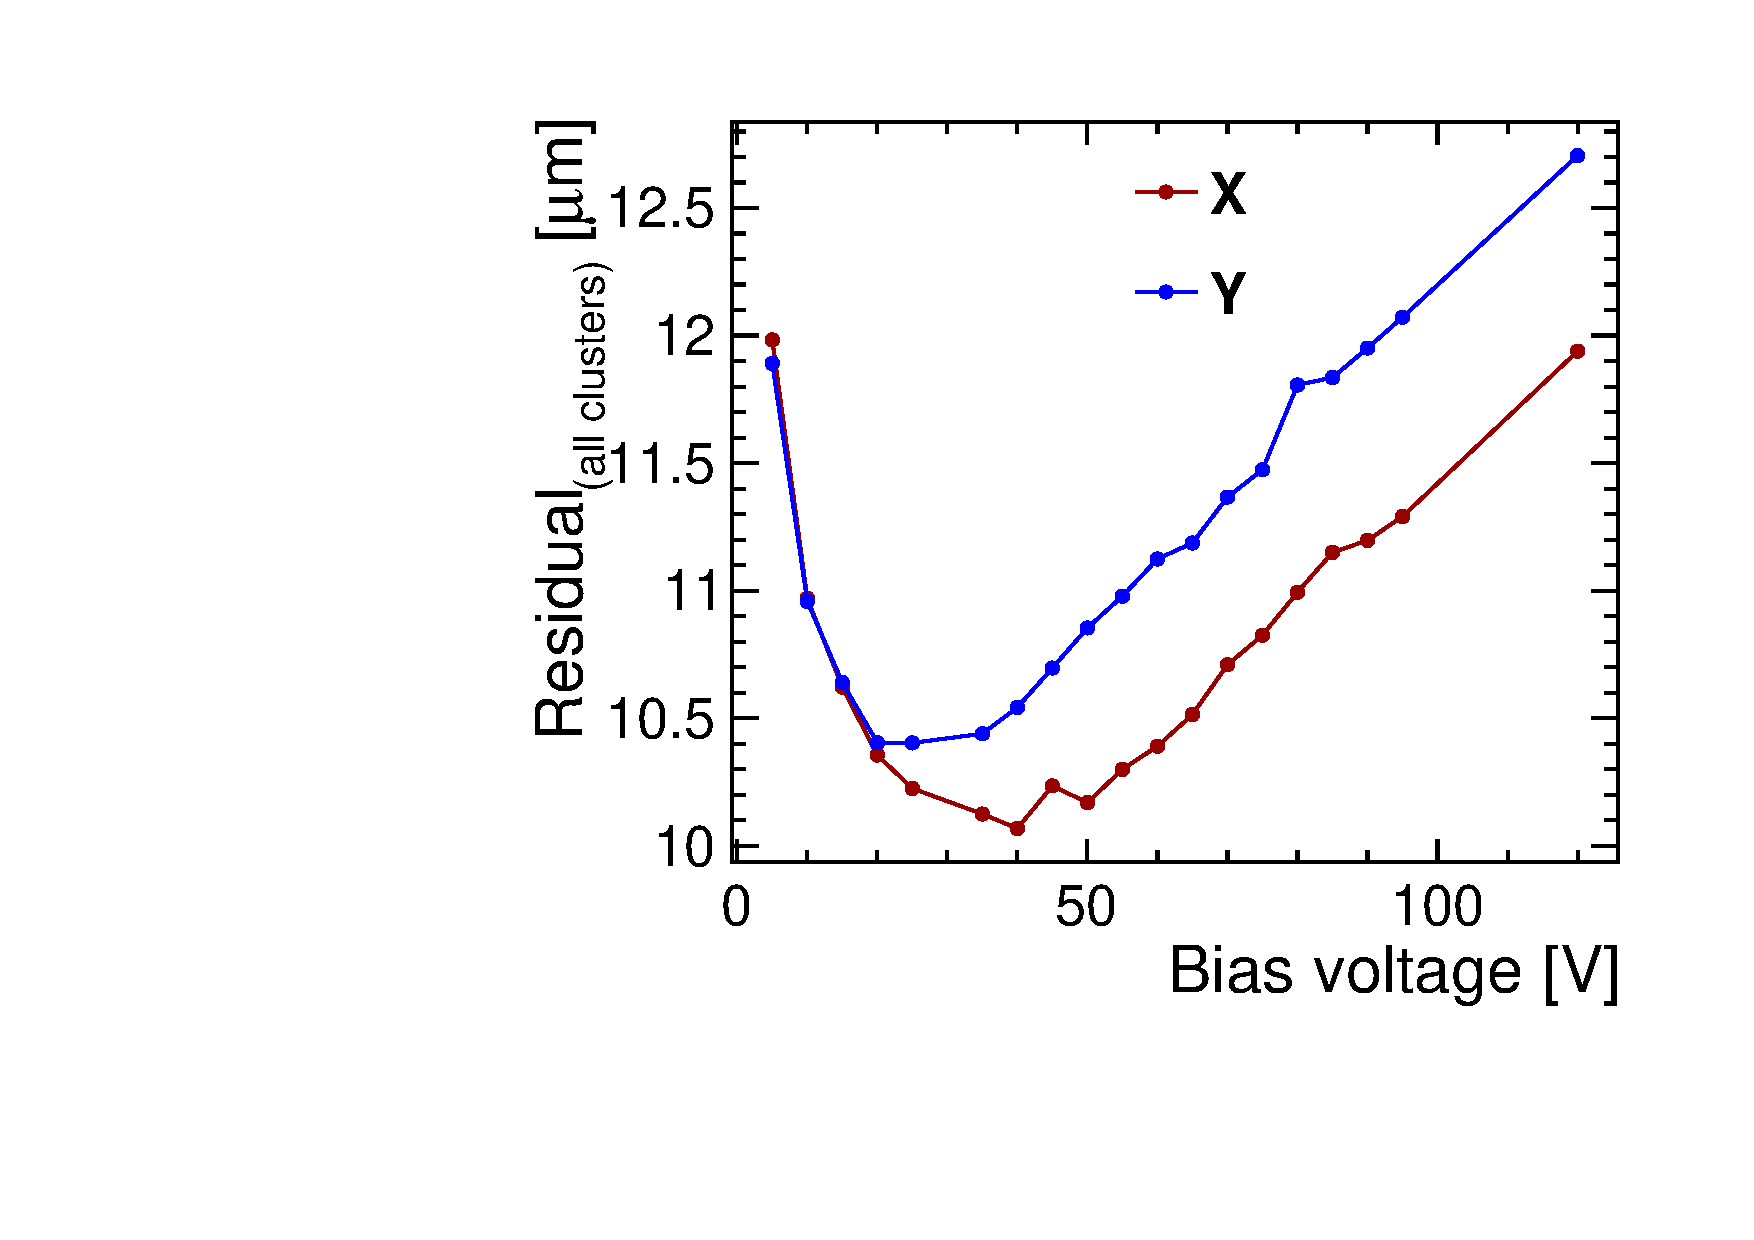
\includegraphics[width=\textwidth]{./figures/TestBeam/W2_J5_Residual_vs_bias.pdf}
%     \caption{W2\_J5}
%   \end{subfigure}
%   \caption{Residuals vs. bias voltage.}
%   \label{fig:Residuals_vs_biasVoltage}
% \end{figure}

% \subsection{Residuals vs. threshold}
% \begin{figure}[htbp] \centering
%   \begin{subfigure}[b]{0.33\textwidth}
%     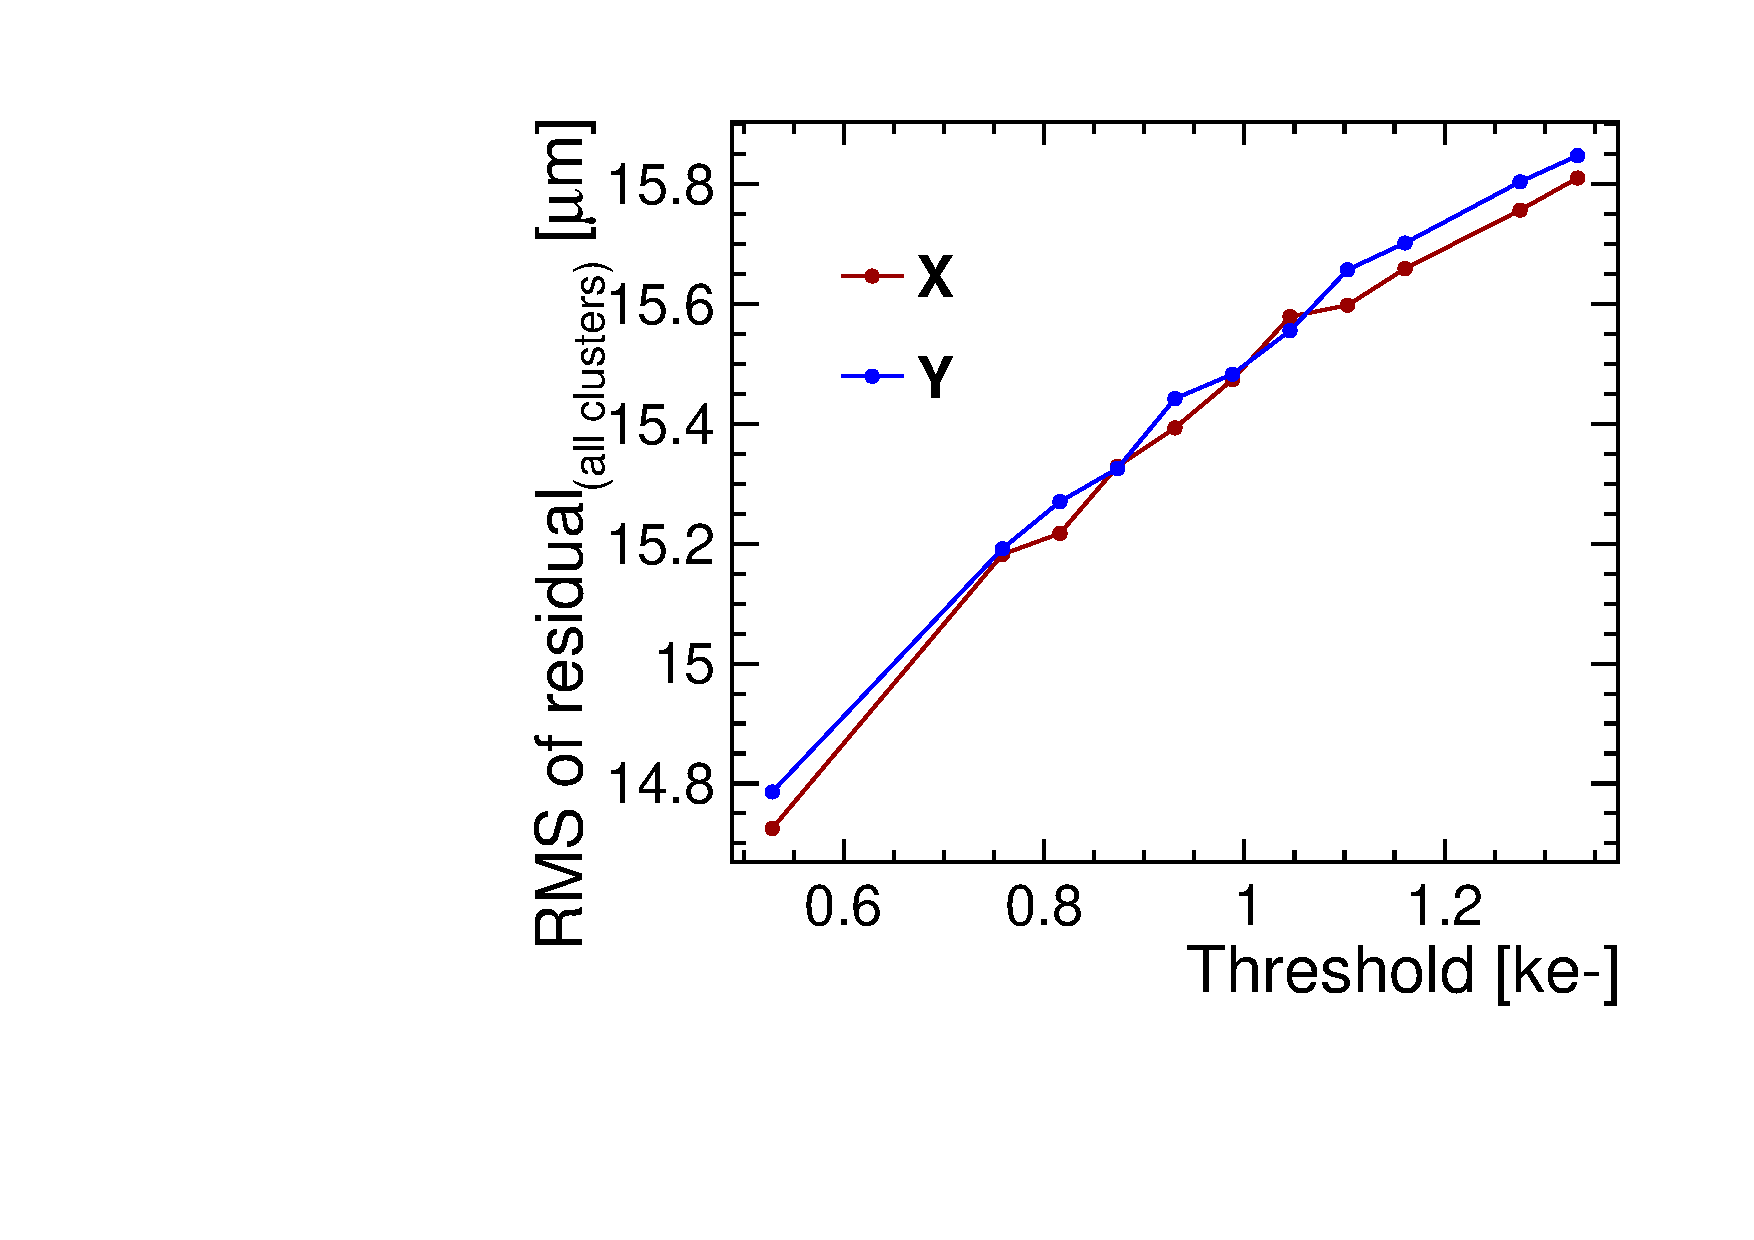
\includegraphics[width=\textwidth]{./figures/TestBeam/residuals_W0019_G07_THLscan.pdf}
%     \caption{20-NGR}
%   \end{subfigure} \hfill
%   \begin{subfigure}[b]{0.33\textwidth}
%     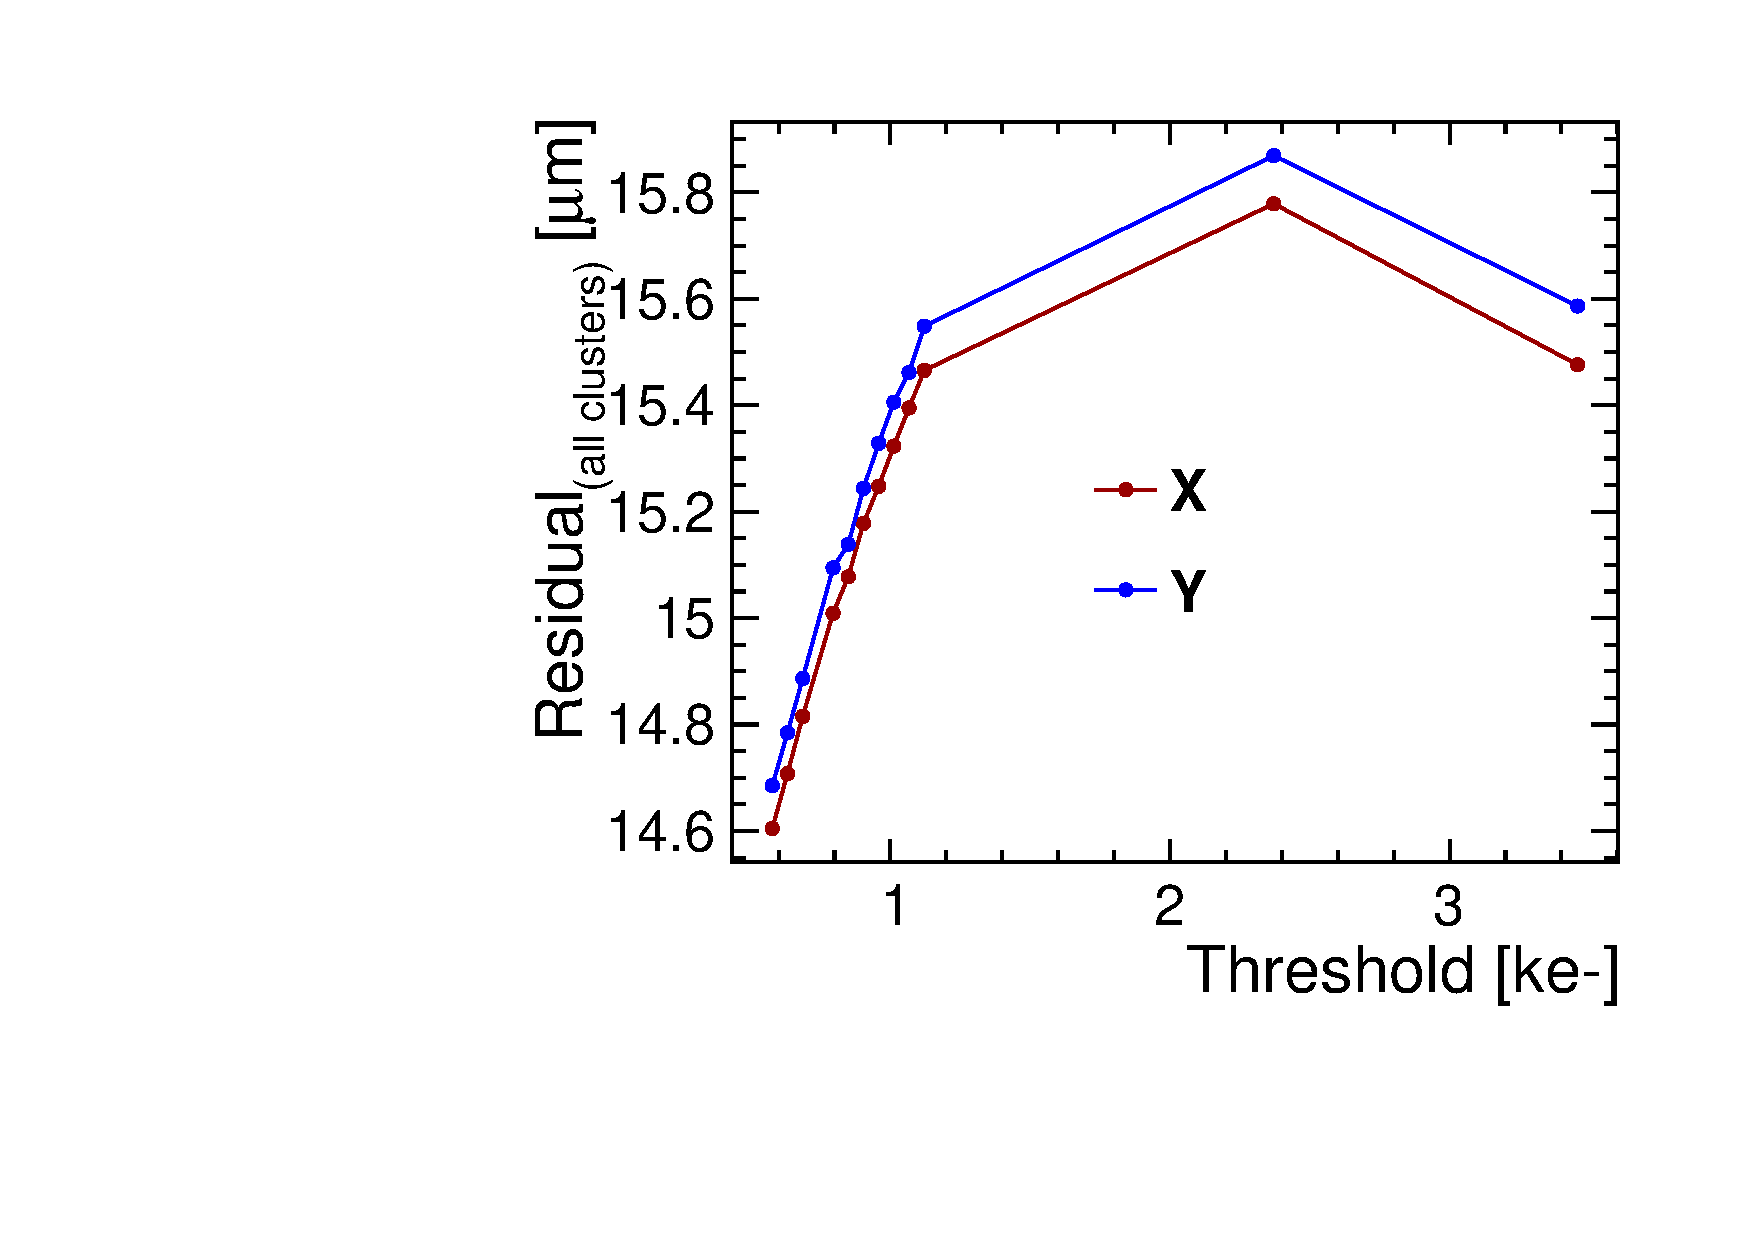
\includegraphics[width=\textwidth]{./figures/TestBeam/residuals_W0019_F07_THLscan.pdf}
%     \caption{23-FGR}
%   \end{subfigure}\hfill
%   \begin{subfigure}[b]{0.33\textwidth}
%     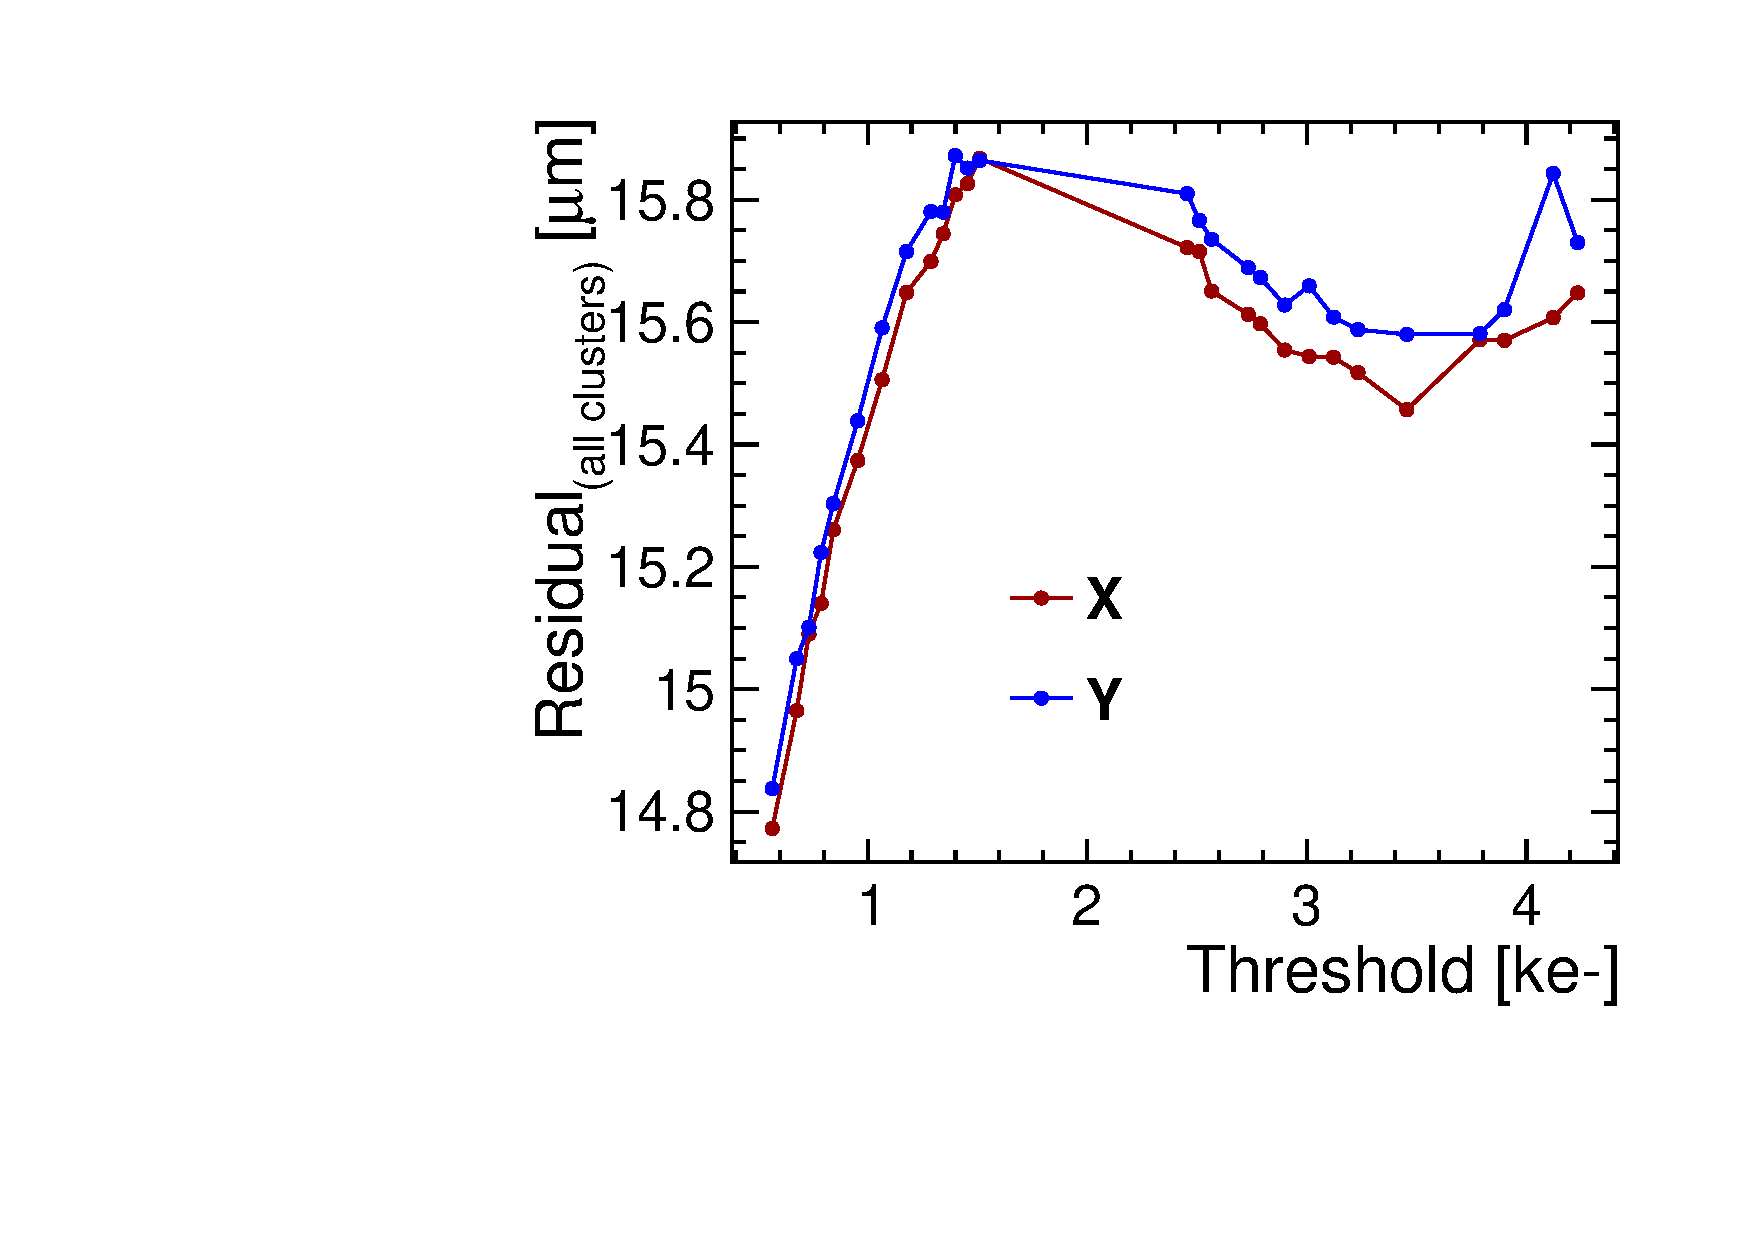
\includegraphics[width=\textwidth]{./figures/TestBeam/residuals_W0019_L08_THLscan.pdf}
%     \caption{28-GNDGR}
%   \end{subfigure} \\

%   \begin{subfigure}[b]{0.33\textwidth}
%     \includegraphics[width=\textwidth]{./figures/TestBeam/residuals_W0019_C07_THLscan.pdf}
%     \caption{55-GNDGR}
%   \end{subfigure} \hfill
%   \begin{subfigure}[b]{0.33\textwidth}
%     \includegraphics[width=\textwidth]{./figures/TestBeam/residuals_W0005_E02_THLscan.pdf}
%     \caption{55-GND-GR-100}
%   \end{subfigure}\hfill
%   \begin{subfigure}[b]{0.33\textwidth}
%     \includegraphics[width=\textwidth]{./figures/TestBeam/residuals_W0005_F01_THLscan.pdf}
%     \caption{55-GND-GR-150}
%   \end{subfigure}\\
%   \begin{subfigure}[b]{0.33\textwidth}

%     \caption{W2\_J5}
%   \end{subfigure}
%   \caption{Residuals vs. threshold.}
%   \label{fig:Residuals_vs_Threshold}
% \end{figure}

% \newpage



%% \begin{figure}[htbp] \centering
%%   \begin{subfigure}[b]{0.45\textwidth}

%%     \caption{}
%%   \end{subfigure} \hfill
%%   \begin{subfigure}[b]{0.45\textwidth}
%%     \includegraphics[width=\textwidth]{./figures/TestBeam/depletionVoltage_W0002_J05.pdf}
%%     \caption{}
%%   \end{subfigure}
%%   \caption{W2\_J5}
%%   \label{fig:W2_J5_depletion}
%% \end{figure}
